\documentclass[master=mai,masteroption=bda]{kulemt}
\setup{title={Image-text Alignment for Artworks},
  author={Feiyang Tang},
  promotor={Prof.\,dr.\,ir.\ Marie-Francine Moens},
  assessor={Prof.\,dr.\,ir.\ Tinne Tuytelaars},
  assistant={Ir.\ Shurong~Sheng}}
% The following \setup may be removed entirely if no filing card is wanted
%\setup{filingcard,
%  translatedtitle=,
%  udc=621.3,
%  shortabstract={Here comes a very short abstract, containing no %more than 500
%    words. \LaTeX\ commands can be used here. Blank lines (or %the command
%    \texttt{\string\pa r}) are not allowed!
%    \endgraf \lipsum[2]}}
% Uncomment the next line for generating the cover page
%\setup{coverpageonly}
% Uncomment the next \setup to generate only the first pages (e.g., if you
% are a Word user.
%\setup{frontpagesonly}

% Choose the main text font (e.g., Latin Modern)
\setup{font=lm}

% If you want to include other LaTeX packages, do it here. 

% Finally the hyperref package is used for pdf files.
% This can be commented out for printed versions.
%\usepackage[pdfusetitle,colorlinks,plainpages=false]{hyperref}
\usepackage{caption}
\usepackage{eucal}
\usepackage{amsmath}
\usepackage{graphicx}
\usepackage{wrapfig}
\usepackage{lscape}
\usepackage{rotating}
\usepackage{epstopdf}

%%%%%%%
% The lipsum package is used to generate random text.
% You never need this in a real master's thesis text!
\IfFileExists{lipsum.sty}%
 {\usepackage{lipsum}\setlipsumdefault{11-13}}%
 {\newcommand{\lipsum}[1][11-13]{\par And some text: lipsum ##1.\par}}
%%%%%%%
\usepackage{epigraph}

\usepackage{listings}
\usepackage{xcolor}

\definecolor{codegreen}{rgb}{0,0.6,0}
\definecolor{codegray}{rgb}{0.5,0.5,0.5}
\definecolor{codepurple}{rgb}{0.58,0,0.82}
\definecolor{backcolour}{rgb}{0.95,0.95,0.92}

\lstdefinestyle{mystyle}{
    backgroundcolor=\color{backcolour},   
    commentstyle=\color{codegreen},
    keywordstyle=\color{magenta},
    numberstyle=\tiny\color{codegray},
    stringstyle=\color{codepurple},
    basicstyle=\ttfamily\footnotesize,
    breakatwhitespace=false,         
    breaklines=true,                 
    captionpos=b,                    
    keepspaces=true,                 
    numbers=left,                    
    numbersep=5pt,                  
    showspaces=false,                
    showstringspaces=false,
    showtabs=false,                  
    tabsize=2
}

\lstset{style=mystyle}

\usepackage{hyperref}
\hypersetup{
    colorlinks=true,
    linkcolor=blue,
    filecolor=blue,      
    urlcolor=blue,
    citecolor=blue,
}
%\includeonly{chap-n}
\begin{document}

\begin{preface}
I would first like to thank my promoter Prof. Marie-Francine Moens for giving me this precious opportunity to conduct this intriguing research under the LIIR laboratory in KU Leuven. Many thanks to my daily advisor Shurong Sheng. The door to her office was always open whenever I ran into a trouble spot or had a question about my research or writing. She consistently allowed this thesis to be my work but steered me in the right direction whenever she thought I needed it.

I would also like to acknowledge Prof. Tinne Tuytelaars as the assessor of this thesis, and I am truly gratefully indebted to her for her very valuable comments on this thesis.

Finally, I must express my very profound gratitude to my mum and to my friends Lieven, Jinjiu, Nanxu and Shuxian for always making me feel at home here in Belgium, providing me with unfailing support and continuous encouragement throughout this year and through the process of researching and writing this thesis. This accomplishment would not have been possible without them. To rest of my family and friends in New Zealand and China, thanks for your comfort calls and endless support. Thank you all.

\end{preface}

\tableofcontents*

%% Shurong: this abstract can be more clear, for example first introduce the motivation to do this work: online data incomplete, facilitate user's experience in museums and so on, and then explain what you have done in this thesis: we target two tasks: coarse-grained level cross modal retrieval and fine-grained cross modal retrieval. We have applied an attention-based approach to conduct the two tasks on two benchmark datasets and achieved acceptable results. you can here give more detailed explanation on the approach. [done]

%%!!shurong: double check the results. the text for Egyptian is more noisy, it is more logical that the Chinese dataset has better results.

%%SHURONG: DOUBLE CHECK THE TYPOS AND GRAMMARS. MY ENGLISH IS NOT NOT GOOD EITHER, COULD BE NICE IF THERE IS A NATIVE ENGLISH SPEAK TO PROOFREADING THE THESIS
\begin{abstract}
With the rapid development of the Internet in the past decades, everything around us has begun to be gradually digital. The recent pandemic of COVID-19 has made everyone realise the importance and convenience of going digital. For example, while we are staying at home, we can enjoy the master's masterpieces without leaving the house by browsing websites of popular art exhibitions and museums. However, there are many challenges in the field, such as the uncompleted online data, and the limited user experience in the museum. To provide users with a better experience, we need to effectively annotate artworks to describe artwork image or sub-image with its textual attributes automatically. Therefore, this thesis targets two tasks: coarse-grained level cross modal retrieval and fine-grained cross modal retrieval. Recently, there is an interest in finding all potential alignments between the image area and the word at the same time using cross attention, thereby calculating the similarity of the text. 
%SHURONG: This cross attention based work has also been proved to excel and surpass other techniques in the task of image-text alignment for natural image.[done]
This cross attention-based work has also been proved to excel and surpass other techniques in the task of image-text alignment for natural image. We have adopted this attention-based approach to conduct these two tasks on two benchmark datasets and achieve acceptable results. Our presented framework supports annotating artworks in an automatic mode and
provides descriptions between image/sub-image and textual attributes in either a coarse-grained or fine-grained level.


%%Most studies on multimodal information retrieval conduct the process on the image or sentence level, often used training set and models based on natural images. However, current research has shown that we need to move beyond the traditional coarse-grained multimodal information retrieval model in order to effectively annotating artworks to describe artwork image or sub-image with its textual attributes automatically. Recently, there is an interest in finding all potential alignments between the image area and the word at the same time using cross attention, thereby calculating the similarity of the text. This work has been proved its ability to excel and surpass other techniques in the task of image-text alignment. Nevertheless, one limitation is that these works do not consider those images which may have different representations and subtle features, e.g. artworks. Achieving image-text alignment in a find-grained level requires us to develop an efficient and effective mechanism to address the subtle and detailed features in artworks image and sentence fragments. In our research, we concentrate on fragment level image and sentence retrieval. We present a comprehensive framework for aligning fine-grained image-text from artworks. This supports annotating artworks in an automatic mode and provide descriptions between image or sub-image and textual attributes as precise as possible.

\end{abstract}

% A list of figures and tables is optional
%\listoffigures
%\listoftables
% If you only have a few figures and tables you can use the following instead
\listoffiguresandtables
% The list of symbols is also optional.
% This list must be created manually, e.g., as follows:
\chapter{List of Abbreviations}
\section*{Abbreviations}
\begin{flushleft}
  \renewcommand{\arraystretch}{1.1}
  \begin{tabularx}{\textwidth}{@{}p{12mm}X@{}}
    ILSVRC & ImageNet Large Scale Visual Recognition Challenge \\
    FDDB   & Face Detection Data Set and Benchmark \\
    LFW   & London Fashion Week Data \\
    RCNN  & Region Convolutional Neural Network \\
    SS   & Seletive Search algorithm \\
    RPN & Region Proposal Network \\
    YOLO & You Only Look Once algorithm \\
    SOTA & State of the Art (the best) \\
    CNN & Convolutional Neural Networks \\
    VGG & Very Deep Convolutional Networks for Large-Scale Visual Recognition \\
    SCAN & Stacked Cross Attention \\
    ResNet & Residual Neural Network \\
    GRU & Gated Recurrent Unit
  \end{tabularx}
\end{flushleft}
%\section*{Symbols}
%\begin{flushleft}
%  \renewcommand{\arraystretch}{1.1}
%  \begin{tabularx}{\textwidth}{@{}p{12mm}X@{}}
%    42    & ``The Answer to the Ultimate Question of Life, the Universe,
%            and Everything'' according to \cite{h2g2} \\
%    $c$   & Speed of light \\
%    $E$   & Energy \\
%    $m$   & Mass \\
%    $\pi$ & The number pi \\
%  \end{tabularx}
%\end{flushleft}

% Now comes the main text
\mainmatter

\chapter{Introduction}
\label{cha:intro}

%\epigraph{\textit{``If we want machines to think, we need to teach them to see.''}}{\textit{- Li Fei-Fei}}

%% shurong: replace this part (til the end of 1.1) by some introductions on image-text alignment and cross modal retrieval

As a part of the millions of internet users who often surf on the internet, we always ``Google'': enter the keywords to be searched to retrieve our desired text information, which is to retrieve text with text in this case. Sometimes we also upload images on Google to find similar ones, which refers to using an image to retrieve images. However, considering the situation when we use textual information to retrieve images on Google, at this time the type of information we enter and the type of information obtained is different, known as ``cross modal''.

Cross modal retrieval can be understood as finding the relationship between different modal samples and using a particular modal sample to search for other modal samples with approximate semantics. For example: use the image to retrieve the corresponding text, or use the text to retrieve the desired image. Of course, modals are not limited to images and text, such as voice, physiological signals, and video can be used as components of cross modal retrieval.

The goal of cross modal retrieval is to calculate the similarity between different modal data. For a given query sample, retrieve different modal data related to the query sample. The key challenge lies in the inconsistent representation of different modalities, making it difficult to directly measure the similarity, that is, the ``semantic gap'' problem. There are two mainstream cross-modal retrieval methods: common space learning methods and cross-modal similarity measurement methods.

The common space learning method enables a cross-modal similarity to be directly measured in this space by learning a unified common space for different modal data, mainly including traditional statistical association analysis methods, deep learning based methods, graph-based reduction Methods, metric learning methods, ranking learning methods, dictionary learning methods, cross modal hashing methods, etc.

The cross modal similarity measurement method does not learn the common space, but directly calculates the cross modal similarity, mainly including graph-based methods and nearest neighbour analysis methods. Besides, there are some other cross modal retrieval methods, such as correlation feedback analysis method, multi-modal theme model method, etc.

At present, the types of multimedia in cross modal retrieval mainly include images, text, voice, video and 3D graphics. Most cross modal retrieval methods are currently limited to the use of images and text, as well as a small number of other types of voice and video. On the one hand, almost no databases are containing these five modal types; on the other hand, there are ``semantic gaps'' in the various forms of different modal types.

The ``semantic gap'' problem is a core challenge faced by cross-modal retrieval: data of different modalities have different feature representations, and their similarity is difficult to measure directly. In order to solve the above problem, an intuitive method is to unify the representation across modalities, that is, to map different modal data from their independent representation spaces into a third-party, public space so that they can measure the similarity of each other. In recent years, with the rapid development and broad application of deep learning, the unified representation method based on deep learning has become a research hot spot and mainstream.

%As the most basic and influential part of human's sensory nervous system, vision plays a vital part in all kinds of recognition tasks. A glance at an image is sufficient for a human to point out and describe an immense amount of details about the visual scene. Traditionally, object recognition and description were performed manually. As time passed, the number of images in many systems grew to more substantial than terabyte size, and could no longer be maintained manually, which brought the idea of machine learning and computer vision also formed a part of artificial intelligence. 

%The process of ``teaching machines to see'' has been widely discussed since the late 20$^{th}$ century and focused on modelling the 3D shape of objects. The latter focus emphasises the identification of objects, and this was achieved by adopting the AdaBoost \cite{adaboost} algorithm. Recently, since neural network-based algorithm AlexNet \cite{alexnet} won the object recognition ImageNet \cite{imagenet} competition in 2012, the field of computer vision began to make breakthroughs. At present, the top technology in the field of computer vision has been continuously approaching human performance. Besides, the learning mechanism, performance and security of neural networks are discussed in more depth.

%\section{Computer Vision}

%Computer vision (CV) refers to the ability of machines to perceive the environment, and it is the subject of researching machine vision capabilities, or the subject that enables machines to analyse the environment and the stimuli therein visually. Machine vision usually involves the evaluation of images or videos. The British Machine Vision Association (BMVA) defines machine vision as "the automatic extraction, analysis, and understanding of useful information from a single image or a series of images." \cite{bmva}

%A real understanding of our environment is not achievable only by visual representation. More precisely, it is the process of transmitting visual cues to the primary visual cortex through the optic nerve, and then being analysed by the brain in a highly characterised form. Extracting explanations from this sensory information contains almost all of our natural evolution and subject experience, that is, how evolution survives us, and how we learn and understand the world in our lifetime.

%In this respect, the visual process is only the process of transmitting images and interpreting them. However, from a computational point of view, the images are closer to thought or cognition and involve many functions of the brain. Therefore, due to the remarkable cross-domain characteristics, many people think that computer vision is a real understanding of the visual environment and its context, and will lead us to achieve reliable artificial intelligence.

\section{Motivation}
%% shurong: extend the motivation in the abstract and emphasize that image-text alignment in the cultural heritage domain has not been a lot exploit yet, they are quite popular for natural images. you can also merge this part with the above part if the content is too less
Image-text alignment is a fundamental research topic in the inter-field of computer vision and natural language processing. It includes two sub-tasks: image annotation and image search. The topic of image-text alignment and cross modal retrieval has been widely discussed in the field of natural images. However, image-text alignment in the cultural heritage domain has not been a lot exploit yet. It can save the intense labour from annotating the artworks for online digital artwork archives if we can automatically describe an artwork image or sub-image with its textual attributes. Furthermore, this topic can help to boost the multi-modal question answering performance in the cultural heritage domain by providing fine-grained image-text correspondence information \cite{mqa}. Therefore, it is interesting to explore the methods that can figure out the artwork image or sub-image and text correspondence.

While a large number of papers discussed aligning image-text and coarse-grained modal information retrieval, the fragment level image-text alignment problem has not been as widely dealt within the multi-modal question-answering research domain. Coarse-grained modal information retrieval can retrieve information between image and text. However, it usually does not work well on artwork datasets which usually contain some fine-grained patterns and objects in one artwork image, therefore reduce the effectiveness of the retrieval model. In this section, we look at two simple examples of ancient Egyptian artworks and how textual description can be generated to match its image.

\begin{figure}[h!]
\centering
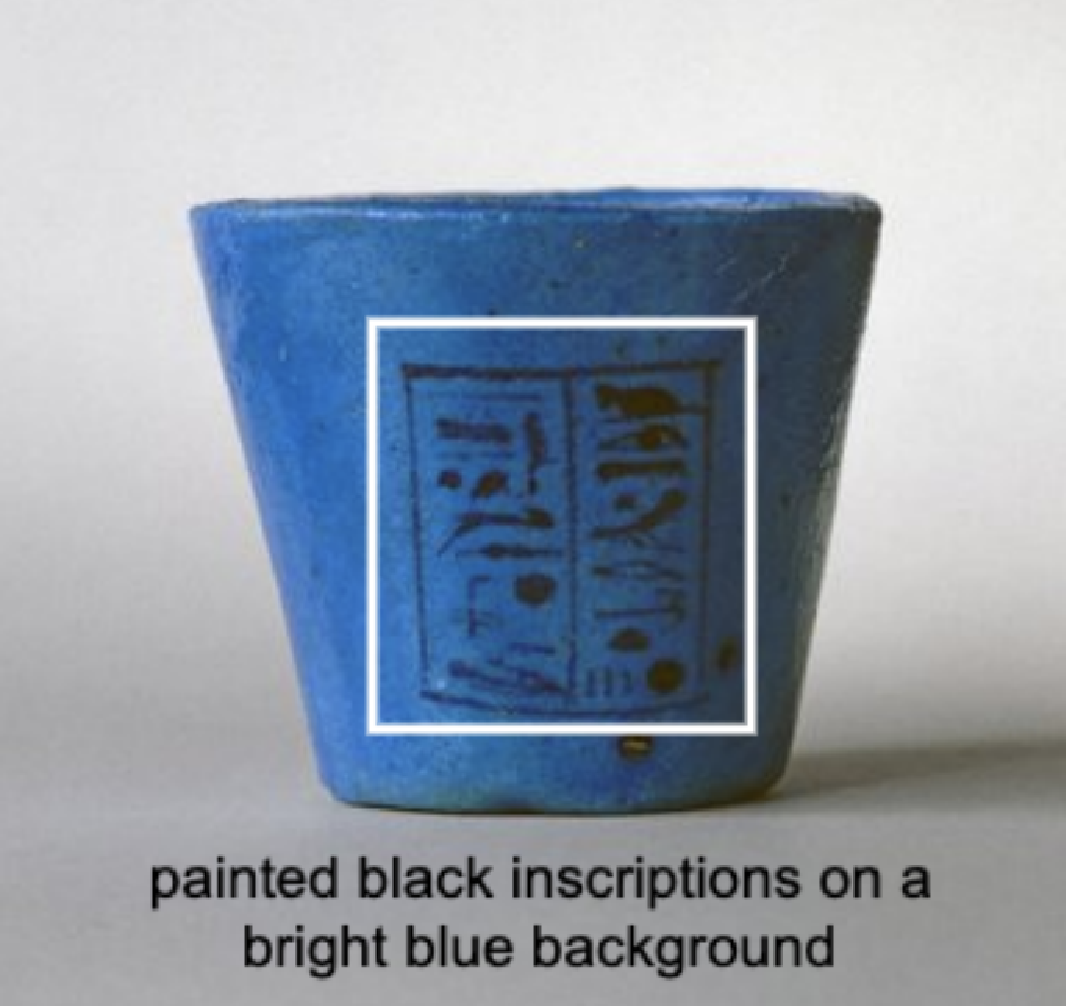
\includegraphics[width=0.35\textwidth]{artwork_fine1.pdf}
\caption{Ancient Egyptian Artwork Example (coarse-grained)}
\label{fig:artwork1}
\end{figure}

Figure \ref{fig:artwork1} shows a small blue container with black inked motifs on it. Using a coarse-grained multi-modal retrieval model, we can generate the textual description ``\textit{painted black inscriptions on a bright blue background}'', which is sufficient enough for this artwork. However, in the real-world scenarios, there is much more likely for us to encounter an artwork showing in Figure \ref{fig:artwork2}. Our traditional coarse-grained multi-modal retrieval model generates ``\textit{a red and a white pot}'' for this artwork but it is not detailed and did not cover sufficient information in the artwork image. Therefore, this motivated us to propose a fine-grained multi-modal retrieval model which can focus on the fragment level image/sentence retrieval. The description on the image was generated by our fine-grained multi-modal retrieval model, which has significantly more detailed information.

\begin{figure}[h!]
\centering
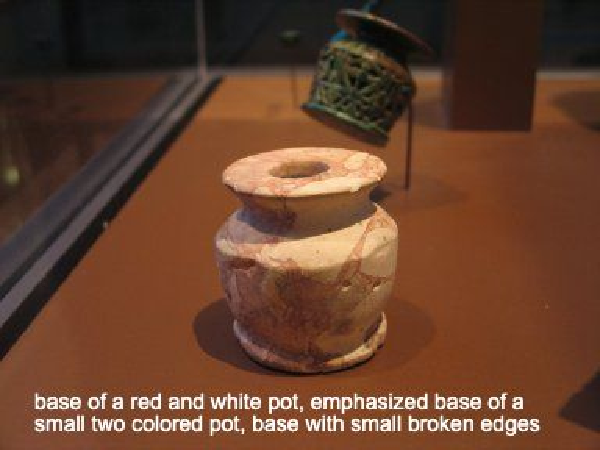
\includegraphics[width=0.45\textwidth]{artwork_fine2.pdf}
\caption{Ancient Egyptian Artwork Example (fine-grained)}
\label{fig:artwork2}
\end{figure}


%% shurong: move the examples in 1.2 to the dataset part. There are also redundant info in this section. double check and remove repeated content
\section{Dataset}

The datasets \cite{artworkcaption} involved in this thesis research are collected from the following online sources: the Brooklyn Museum \cite{brooklynmuseum}, the Metropolitan Museum \cite{themet}, and the British Museum \cite{thebritishmuseum}. Based on these sources, we have created two artwork datasets: the ancient Egyptian art image dataset and the ancient Chinese art image dataset. The two datasets are collected based on the geographical location of the origin of the artworks because caption words may differ much depending on the cultural background of the location. Detailed statistics of the two datasets are shown in Table \ref{fig:datasetstats}. 

\begin{table}[h!]
\centering
\begin{tabular}{|c|c|c|c|}
\hline
\textbf{Dataset}          & \textbf{Num. of Artworks} & \textbf{Aver. Length} & \textbf{Num. of Tokens} \\ \hline
\textbf{Egyptian} & 16,146                       & 9                       & 10,694                     \\ \hline
\textbf{Chinese}  & 6,847                        & 10                      & 4,721                      \\ \hline
\end{tabular}
\caption{Statistics of Our Datasets \cite{artworkcaption}}
\label{fig:datasetstats}
\end{table}

The datasets have 22,993 high-quality artwork images recorded
in a controlled setting. Images are stored at varying dpi and the
compressed \verb|jpeg| image file size ranges between 20-300 KB. The paragraph-level descriptions are split into multiple sentences and a maximum of five sentences are retained for each artwork to reduce data imbalance. In addition, we removed noisy texts from the captions following a specific pattern, e.g, ``See 13.26.59'' \cite{artworkcaption}. The number is the accession number of an artifact that obviously cannot be derived from the input image or artwork type. We also remove duplicate images in the captioning datasets based on their hash code. Tokens occurring less than two times are removed from the training vocabulary. The datasets are all split into an 80\%, 10\%, and 10\% partition for respectively training, validation, and test.

Each artwork image has a corresponding record saved in a \verb|json| file containing their processed caption textual data. However, in our research, instead of using the original captions in the \verb|json| file, we extracted noun phrases from them and performed our alignment tasks between these noun phrases and images.

Here we focus on ancient Egyptian and Chinese artworks; we manually construct our datasets; they consist of 16,146 images from Egyptian domain and 6,847 images in Chinese. Figure \ref{fig:sampleEgyptian} and Figure \ref{fig:sampleChinese} show three examples of artworks from the Egyptian and Chinese collection with textual captions.

\begin{figure}[h!]
\centering
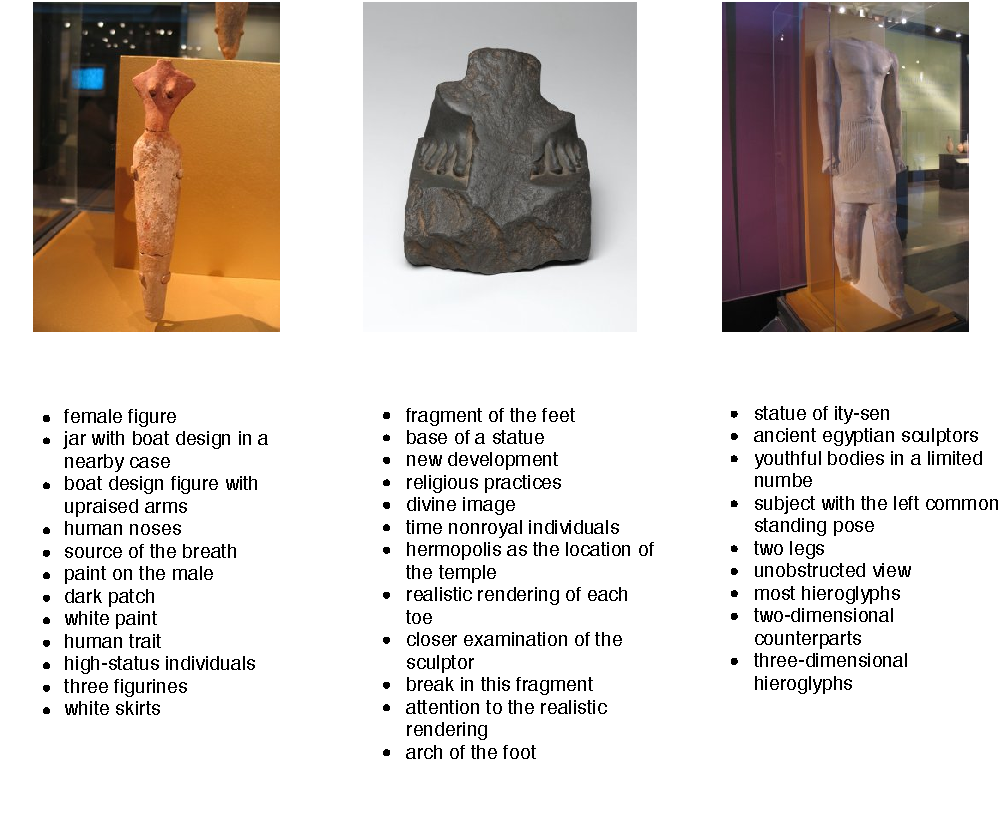
\includegraphics[width=0.9\textwidth]{egyptian.pdf}
\caption{Examples of Artworks of Egyptian Artwork Dataset}
\label{fig:sampleEgyptian}
\end{figure}

\begin{figure}[h!]
\centering
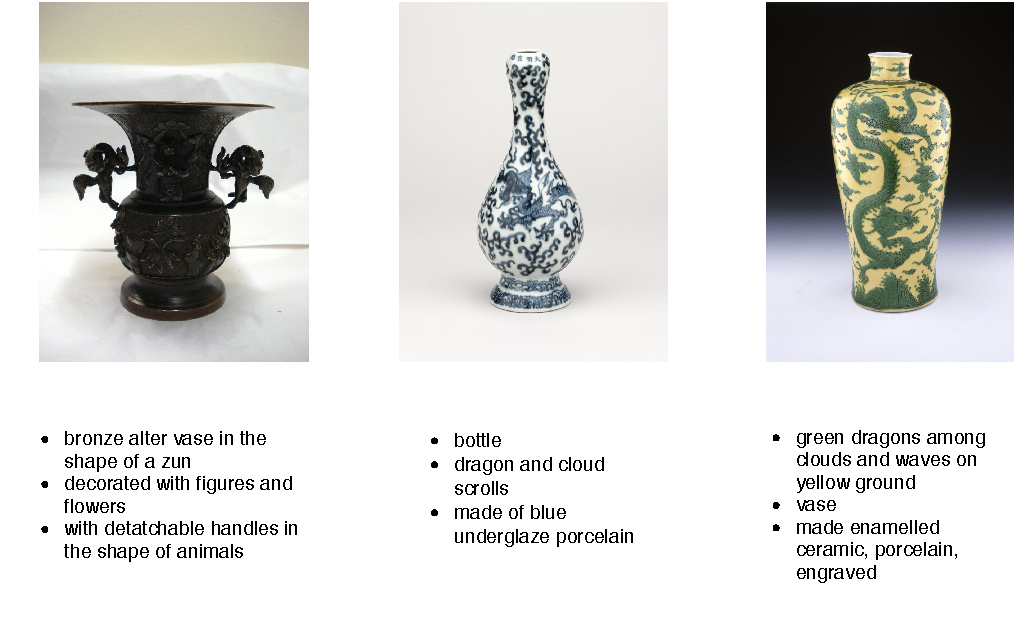
\includegraphics[width=\textwidth]{chinese.pdf}
\caption{Examples of Artworks of Chinese Artwork Dataset}
\label{fig:sampleChinese}
\end{figure}

\section{Research Questions}

In this thesis, we study fine-grained image-text alignment for artworks. Fine-grained image-text alignment refers to the fragment level cross modal (between image and text) retrieval. The prior sections list the background and motivations, the specific research questions that we look at are:

%% two research questions: 1. is the alignment model experimented on natural images effective for artwork items 2. can coarse-grained cross-modal retrieval modal be adapted to fine-grained retrieval and how?
\begin{itemize}
    \item Why mainstream coarse-grained image-text alignment techniques does not suit artwork domains well?
    \item Can we propose a practical approach that facilitates the textual attributes annotation of artwork images accurately and efficiently?
    \item Can we develop a fine-grained image-text alignment technique that can retrieve text from images and vice versa on fragment level?
\end{itemize}

\subsection{Cross Modal Retrieval Framework}

As mentioned above, our primary research task here is to achieve cross modal retrieval (i.e. between image and text) for artworks. Figure \ref{fig:framework} illustrates a brief working framework for the tasks.

%% [solved]shurong: the training data is a bit confusing. an image should be composed of a certain number of image fragments and the text is noun-phrase composed sentence .Or the picture can be kept here but you explain the two levels of retrieval clearly or even give examples.
\begin{figure}[h!]
\centering
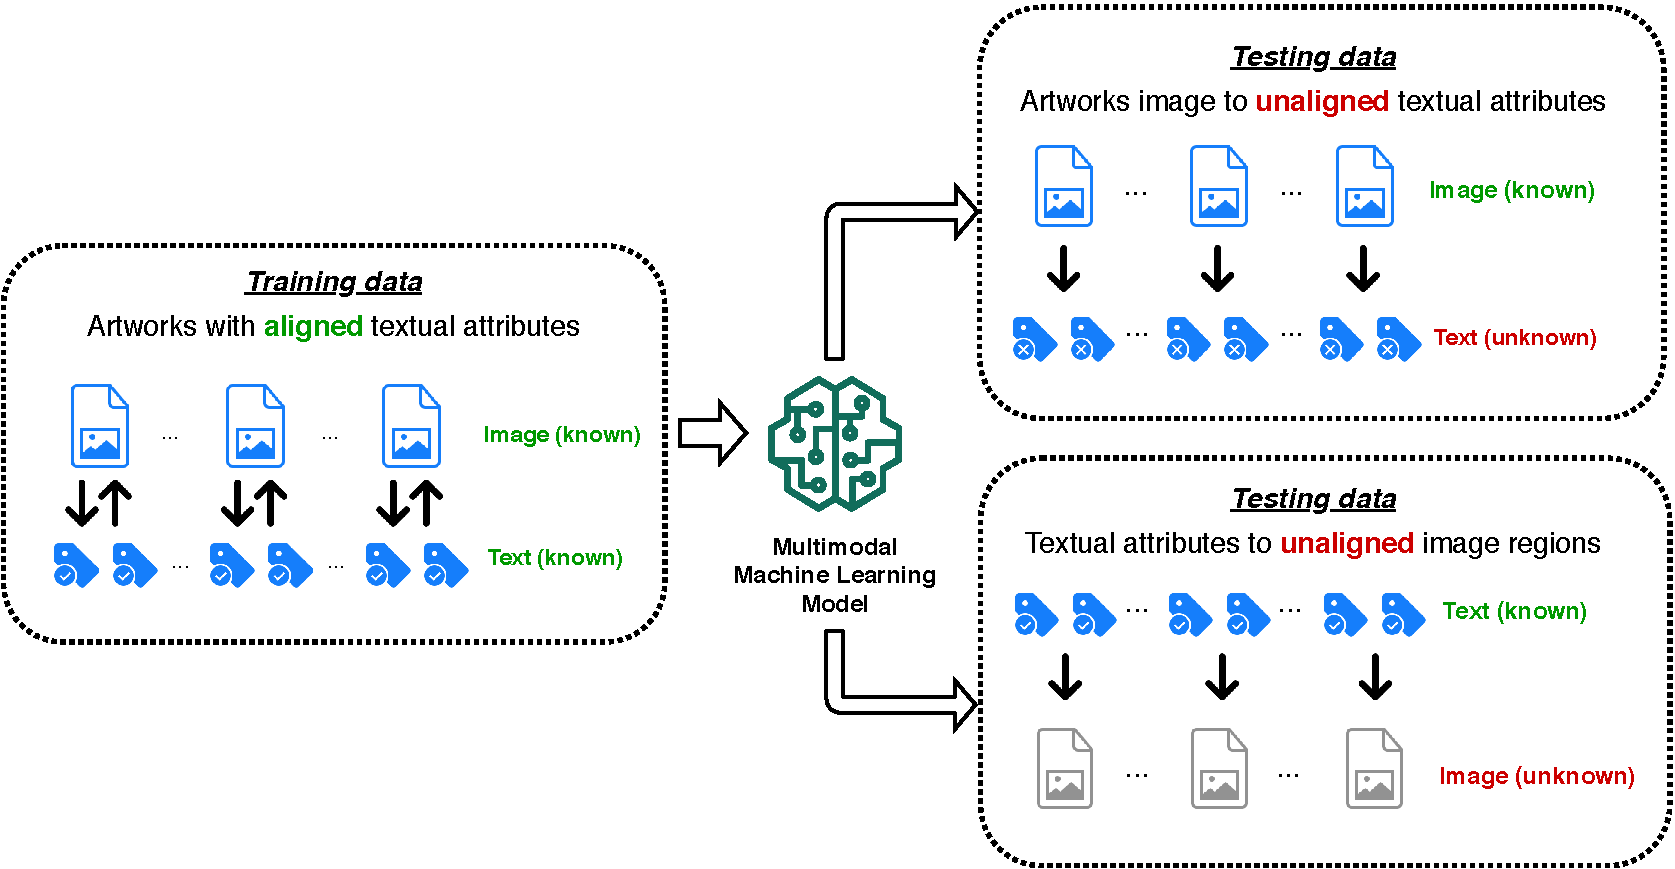
\includegraphics[width=\textwidth]{framework.pdf}
\caption{Cross Modal Retrieval Process}
\label{fig:framework}
\end{figure}

We train our multi-modal machine learning model on the known image features and corresponding textual attributes; this training process helps us learn the potential relationships between image and text. This trained model will be used to generate textual attributes from known image features and vice versa. We believe this may help with automating the artwork annotation process and significantly save labours on artworks classifications and searches.


\section{Contributions}
The main contributions made by this thesis are:

\begin{enumerate}
    \item We review work from several disciplines which may be of relevance to the present subject of inquiry and provide commentary on how the findings from these disciplines may be useful. (Section~\ref{cha:relatedworks})
    \item We adopted SCAN \cite{scan} as the coarse-grained cross modal retrieval model, analysed its structure and applied it on our proposed Egyptian and Chinese artworks datasets to achieve the image-text alignment. By employing this model, we are able to have a coarse-grained alignment between artworks image and textual attributes. This lays the foundation of our improved fine-grained model. (Section~\ref{cha:scan})
    \item By focusing on fragment level image features and textual attributes instead of feeding the whole images and sentences, we are able to perform cross modal retrieval in a more fine-grained level. This allows the future multi-modal retrieval tasks on artworks to achieve more accurate and stable results. (Section~\ref{cha:Method})
\end{enumerate}


\section{Structure of Thesis}

This thesis is structured into the following chapters:

\begin{itemize}
    
    \item \textit{Section~\ref{cha:intro} Introduction}\newline
    We provide the reader with a relevant background to understand this thesis.

    \item \textit{Section~\ref{cha:relatedworks} Related Works}\newline
    We introduce relevant research in image recognition, deep learning, object detection, natural language processing and image-text alignment. In particular, we detail seminal research and review the overall state of the current research. We also review the difference in the works pertaining to the traditional visual-semantic alignment technique versus the more recent cross attention image-text alignment framework.
    
    \item \textit{Section~\ref{cha:scan} Coarse-grained Cross Modal Retrieval}\newline
    We introduce our coarse-grained cross-modal retrieval modal - SCAN, discuss how its components interact with each other and explain how SCAN uses cross attention to improve image-text alignment. We also show the preliminary result running SCAN on our ancient Egyptian and Chinese artwork datasets.
    
    \item \textit{Section~\ref{cha:Method} Fine-grained Cross Modal Retrieval}\newline
    We proposed our improved fine-grained cross modal retrieval model, which now focus more on the fragment level image-text alignment. We then perform several experiments on evaluating the effectiveness of our image generation from text and vice versa by the recall. We also point out the direction of possible future improvements by discussing several recent related publications.
    
    \item \textit{Section~\ref{cha:conclusion} Conclusion}\newline
    We conclude the work and add some final reflections and remarks.
\end{itemize}
%%% Local Variables: 
%%% mode: latex
%%% TeX-master: "thesis"
%%% End: 

\chapter{Related Works}
\label{cha:relatedworks}
Image-text alignment is a fundamental research topic in the inter-field of computer vision and natural language processing. There are many approaches proposed to associate images with textual attributes or vice versa. However, the fielded applications on bidirectional image sentence mapping appear to be relatively few, especially for multi-modal question answering. 

It has been suggested that this is due to the intense labour has been paid on annotating artworks for online digital artwork archives, automated image or sub-image with its textual attributes description could significantly improve the payoff. In this chapter we will survey and summarise the literature of image-text alignment and some proposed applications on multi-modal question answering.

The structure of this chapter is as follows. Section 2.1 discusses the history and some basic knowledge of image recognition. Section 2.2 discusses the preliminaries on deep learning and some mainstream object detection techniques. Section 2.3 explains the definition of image-text alignment and related proposed solutions on that task. Section 2.4 summarises this section.

\section{Image Recognition}
The history of research on image recognition stems from the 1960s when Marvin Minsky, also known as ``the father of Artificial Intelligence'' asked his student Gerald Sussman to ``connect a camera to a computer and do something with it'' \cite{hill}. But with minimal resource, this topic did not get enough attention at first. 

\subsection{Early Researches on Image Recognition}

After entering 1970s, the advent of modern electronic computers gives computers a chance to try to answer what they see through images. Researchers first tried to learn from the same way human look at things. It was generally believed that humans could see and understand things because they could observe things in 3-D with two eyes, which now seems rather absurd. Therefore, researchers believed that for a computer to understand the image it sees, it must first recover the three-dimensional structure of the object from its two-dimensional image. This is the so-called ``three-dimensional reconstruction'' method.

Another inspiration is that it was believed that people could recognise an object, for instance: an apple because people already have a priori knowledge: ``Apples are red, round, and smooth''. If a machine was also established with such a knowledge base, then it could match the images with its knowledge base, and potentially comprehend what it sees corresponding to what it already knew. This is the so-called ``a priori knowledge base'' method. However, this method can only extract very few basic features, which is not very practical.

By the 1990s, image processing hardware technology had made huge progress. Meanwhile, researchers began to design different algorithms: introduction of statistical methods and local feature descriptors, which led to more significant development of computer vision technology and started to be widely used in the industries. In the ``a priori knowledge base'' method, the shape, colour, surface texture, and other characteristics of objects are affected by the viewing angle and the observation environment, and they will change under different angles, different lights, and different occlusions. To solve that dilemma, the proposed new method judges things through identification of local features, and establish a local feature index on objects, which can be more accurately matched even if the perspective or observation environment changes.

After entering the $21^{st}$ century, computer vision develops rapidly thanks to the massive data brought by the rise of the Internet, the advent of digital cameras, and the widespread application of machine learning methods. In the past, many rule-based processing methods have been replaced by machine learning: machines automatically summarise the characteristics of objects from massive data then identify and classify. Many applications are emerging at this stage, including camera face identification, security face recognition and license plate recognition, etc. The accumulation of data has also produced many evaluation data-sets, such as official face recognition and face comparison recognition platforms: \textit{FDDB} and \textit{LFW}. One of the most famous ones is \textit{ImageNet} \cite{imagenet}, which contains 14 million labelled images divided into tens of thousands of categories.


\subsection{Image Recognition with Neural Networks}
After 2010, with the power of deep learning, computer vision technology has experienced explosive growth and industrialisation. With the adoption of neural networks, image recognition tasks can be achieved much more efficient and accurate. Figure \ref{fig:nnexample}. below gives us a straightforward illustration of how neural networks help with image recognition.

\begin{figure}[h!]
\centering
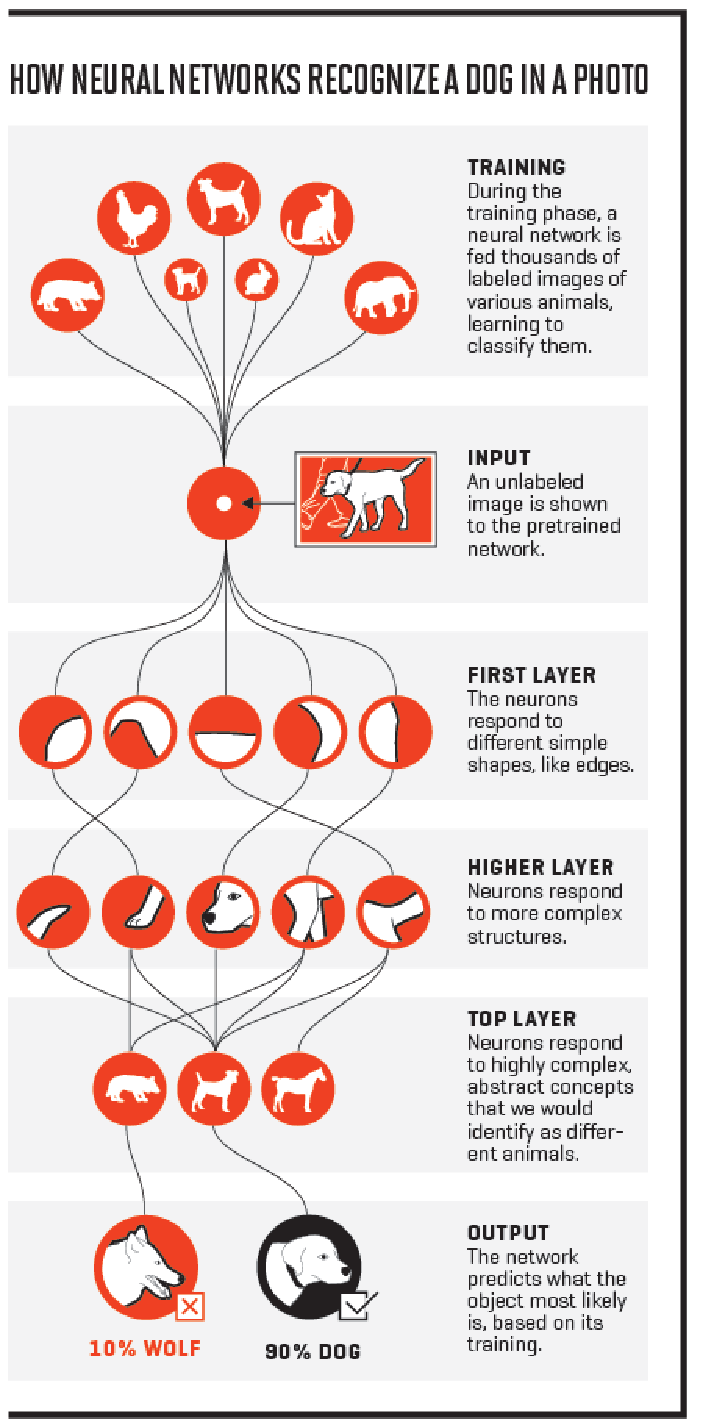
\includegraphics[width=0.4\textwidth]{nnexample.pdf}
\caption{How Neural Networks Performs an Image Recognition Task \cite{parloff_2019}}
\label{fig:nnexample}
\end{figure}

Next, we introduce deep neural networks and how neural networks can be adopted to solve object detection tasks, which is the core part of our project.

\section{Deep Learning and Object Detection}

Through deep neural networks, the accuracy of various types of visual recognition tasks has been dramatically improved. In the well-known computer vision competition ILSVR, the error rate of thousands of object recognition was as high as 25.8\% in 2011. After the introduction of deep learning in 2012, the error rates in the following four years reached 16.4\%, 11.7\%, and 6.7\%, 3.7\%, with significant breakthroughs. Now, face recognition can even achieve a false positive rate of less than one over a million.

Now we know that deep learning has several advantages on image processing and always surpasses other mainstream techniques. But what is deep learning? The following paragraphs give a brief idea of deep learning and how it works.

\subsection{Deep Learning}
In real life, human beings can often solve many problems by intuition. For example, when a human sees Figure \ref{fig:catanddog}. below, he or she can immediately know that there is a cat and a dog in the picture.

\begin{figure}[h!]
\centering
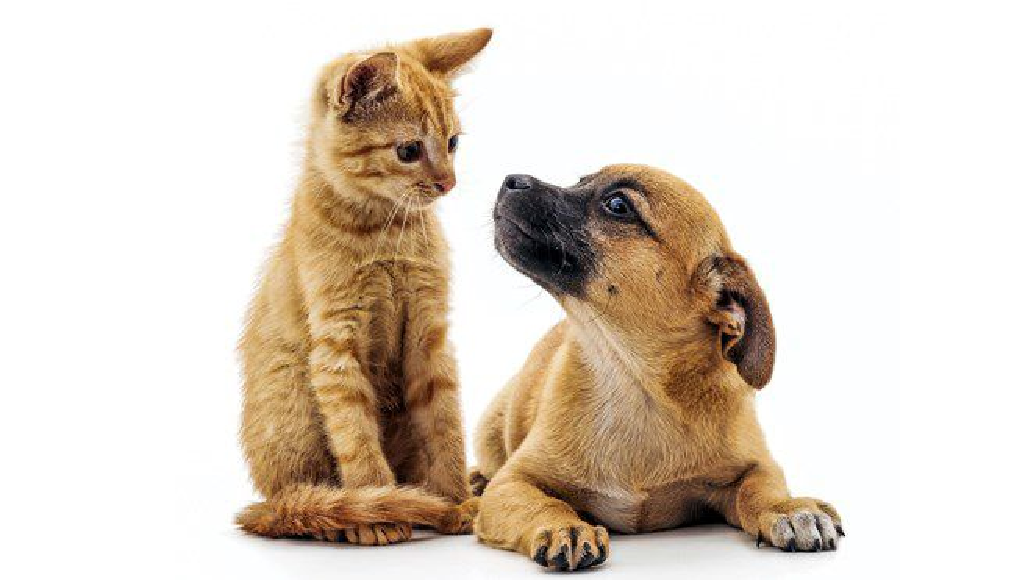
\includegraphics[width=0.4\textwidth]{catanddog.pdf}
\caption{Image of a Cat and a Dog}
\label{fig:catanddog}
\end{figure}

This may feel a natural task for human, but think about how do human know that there are a cat and a dog, but not two cats or two dogs instead? As human can differentiate these two from the picture at a glance, let's try to describe the appearance of cats and dogs. Taking the above picture as an example, we can describe the morphological characteristics of cats as follows: it has a round head, wide cheeks, wide ear roots, deep auricles, and rounded parts at the tip. For the dog in the picture above, its head is flat and wide; the ears are small and thin, the tips of the ears are slightly rounded, the dark apricot eyes, and short hair. Words ``broad cheeks'' and ``round ear tips'' often apply to cats and dogs, while the length of short hair and round ears cannot be quantified with a specific number. When we try to adopt a more specific description like ``dark apricot eyes'', a new problem arises: not all breeds of dogs have such characteristics, but we can still recognise them quickly at a glance.

In short, it is challenging to distinguish cats and dogs accurately with a few words or sentences, but this problem is often solved quickly and accurately by intuition. To solve these seemingly intuitive problems on computers, it is difficult to describe them with specific language or mathematical rules. This brought the invention of deep learning.

Deep learning is to let computers simulate human cognitive processes and learn from experience (also as known as ``intuition''). Make computers understand tasks using a hierarchical concept system like human while each concept is defined by some relatively more straightforward concepts: building simpler concepts to learn complex concepts. The word ``deep'' means more layers of learning system. 

Deep learning has a long and rich history. With the increasing amount of available training data and the continuous improvement of computer software and hardware, the scale of deep learning models has also increased to solve increasingly complex application problems, and the accuracy has continued to increase.



\subsection{Image Understanding}
How to retrieve information out from images that can be understood by a computer has always been the most discussed field of computer vision. Deep learning model have become a popular research area due to its powerful representation capabilities, coupled with the accumulation of data and advances in computing power.

But how to understand an image? There are three main levels according to the needs of subsequent tasks: classification, detection and segmentation. Figure \ref{fig:odsteps}. below provides an example how image understanding tasks can be performed \cite{ouaknine_2018}.

\begin{figure}[h!]
\centering
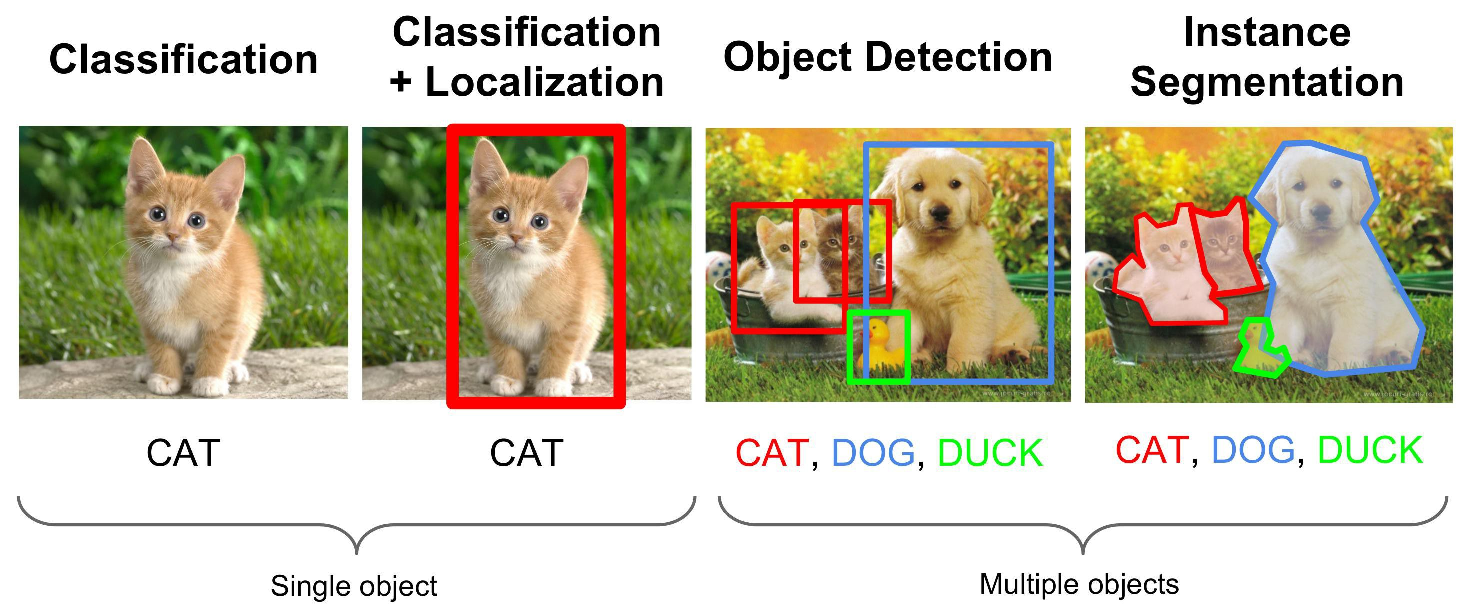
\includegraphics[width=0.7\textwidth]{dlstep.pdf}
\caption{Three Steps of Image Understanding \cite{ouaknine_2018}}
\label{fig:odsteps}
\end{figure}

\subsubsection{Classification}
Classification is the first task, is to structure an image into information of a certain category then describe it by a predetermined category (string) or instance ID. Classification task is the simplest and most basic image understanding task, and it is also the first task for deep learning models to achieve breakthroughs and achieve large-scale applications. In the application field, face recognition and scene recognition can be classified as classification tasks.

\subsubsection{Detection}
The classification task gives the content description of the entire picture, while the detection focuses on the specific object target, which requires the category information and position information of the target to be obtained at the same time. Comparing to the classification task, detection gives an understanding of both foreground and background of the image. To perform detection, we need to separate the interesting targets from the background and determine the description, i.e. category and location of this target. Therefore, the output of this detection model is a list, each item of the list uses a data set to give the category and position of the detected target, which is commonly represented by the coordinates of a rectangular detection frame.

\subsubsection{Segmentation}
Segmentation includes semantic segmentation and instance segmentation. The former is an extension of the previous background separation and requires the separation of image parts with different semantics, while the latter is an extension of the detection task and requires the outline of the target which is finer than the detection frame. Segmentation is a pixel-level description of an image. It gives meaning to each pixel category, i.e. instance and is suitable for understanding demanding scenes, such as the segmentation of roads and non-roads in driver-less technology.

\subsection{Object Detection}

After familiarised the steps of image understanding, in this section we focus on the second task: object detection, which is also the main task of our proposed work. The following paragraph will provide several mainstream models on solving object detection tasks.

\subsubsection{CNN}
First we start with introducing a series of commonly used models called convolutional neural networks (CNN). 

%convolution
\paragraph{Convolution Process}
The convolution process is based on a small matrix, that is, a convolution kernel. The pixel matrix of each layer mentioned above is continuously scanned in steps, the scanned number is multiplied by the number of the corresponding position of the convolution kernel, and then the sum is calculated. Each time you scan, you get a value, and after all the scans, a new matrix is generated. The following Figure \ref{fig:convolutionprocess} illustrates an example of convolution process in a CNN model:

\begin{figure}[h!]
\centering
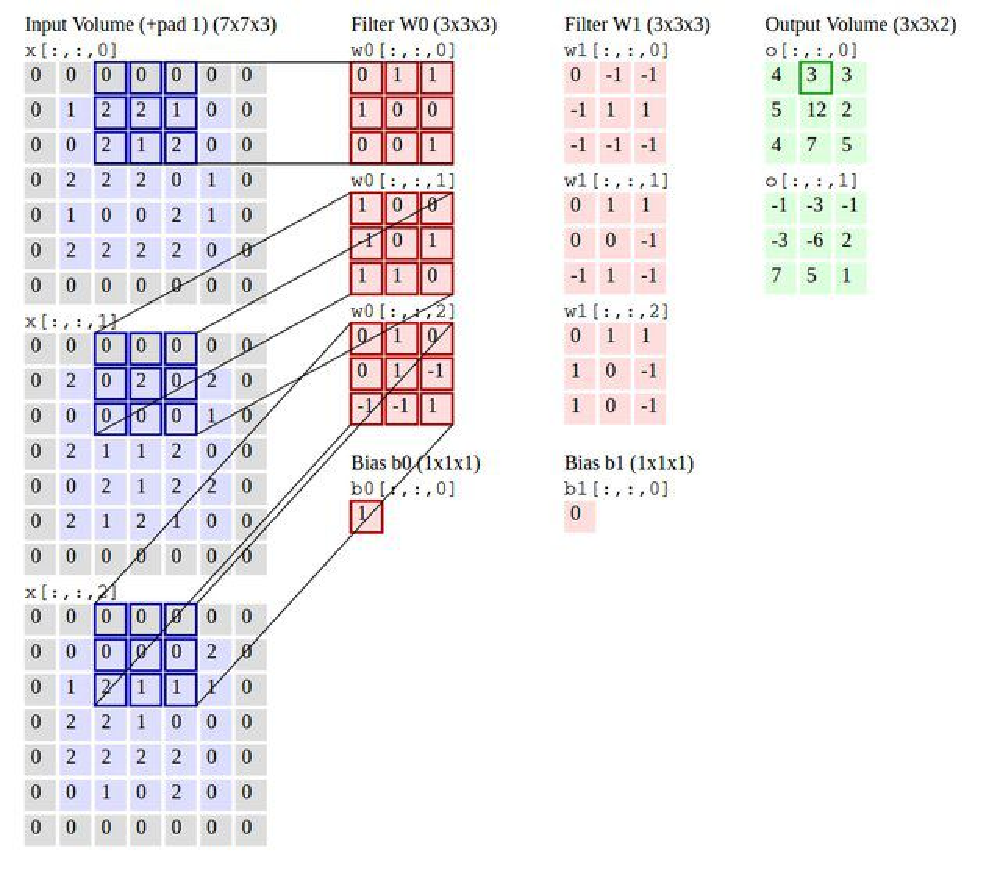
\includegraphics[width=0.7\textwidth]{Convolution_Process.pdf}
\caption{Example of Convolution Process \cite{cnn1}}
\label{fig:convolutionprocess}
\end{figure}

%How to set the convolution kernel can refer to the size and number of the convolution kernel of the convolutional neural network, and 
How to determine the number of convolution layers? Normally we take a small matrix of $(3,3)$. Each value in the convolution kernel is the neuron parameter (i.e. weight) that we need to find (i.e. train). At the beginning, there will be an initial value randomly. When training the network, the network will pass after These parameter values are continuously updated to the propagation until the best parameter value is found. But how do we know which is the ``best'', this is evaluated by a loss function.

The step size of the convolution kernel refers to the movement of the convolution kernel by several grids at a time, with horizontal and vertical directions.

The convolution operation is equivalent to feature extraction, and the convolution kernel is equivalent to a filter to extract the features we need.

%padding
\paragraph{Padding}
After the convolution operation, the dimensions become smaller, and the resulting matrix is smaller than the original matrix, which is difficult to calculate and hard to perform convolution, thus, we need padding. 

Before each convolution operation, we need to wrap a layer of 0 outside the original matrix. It is possible to only fill in horizontally, or only vertically, or 0 on all sides, so that after convolution, the size of output image will be consistent with input image. Figure \ref{fig:padding} below gives an example of padding zeros to an image.

\begin{figure}[h!]
\centering
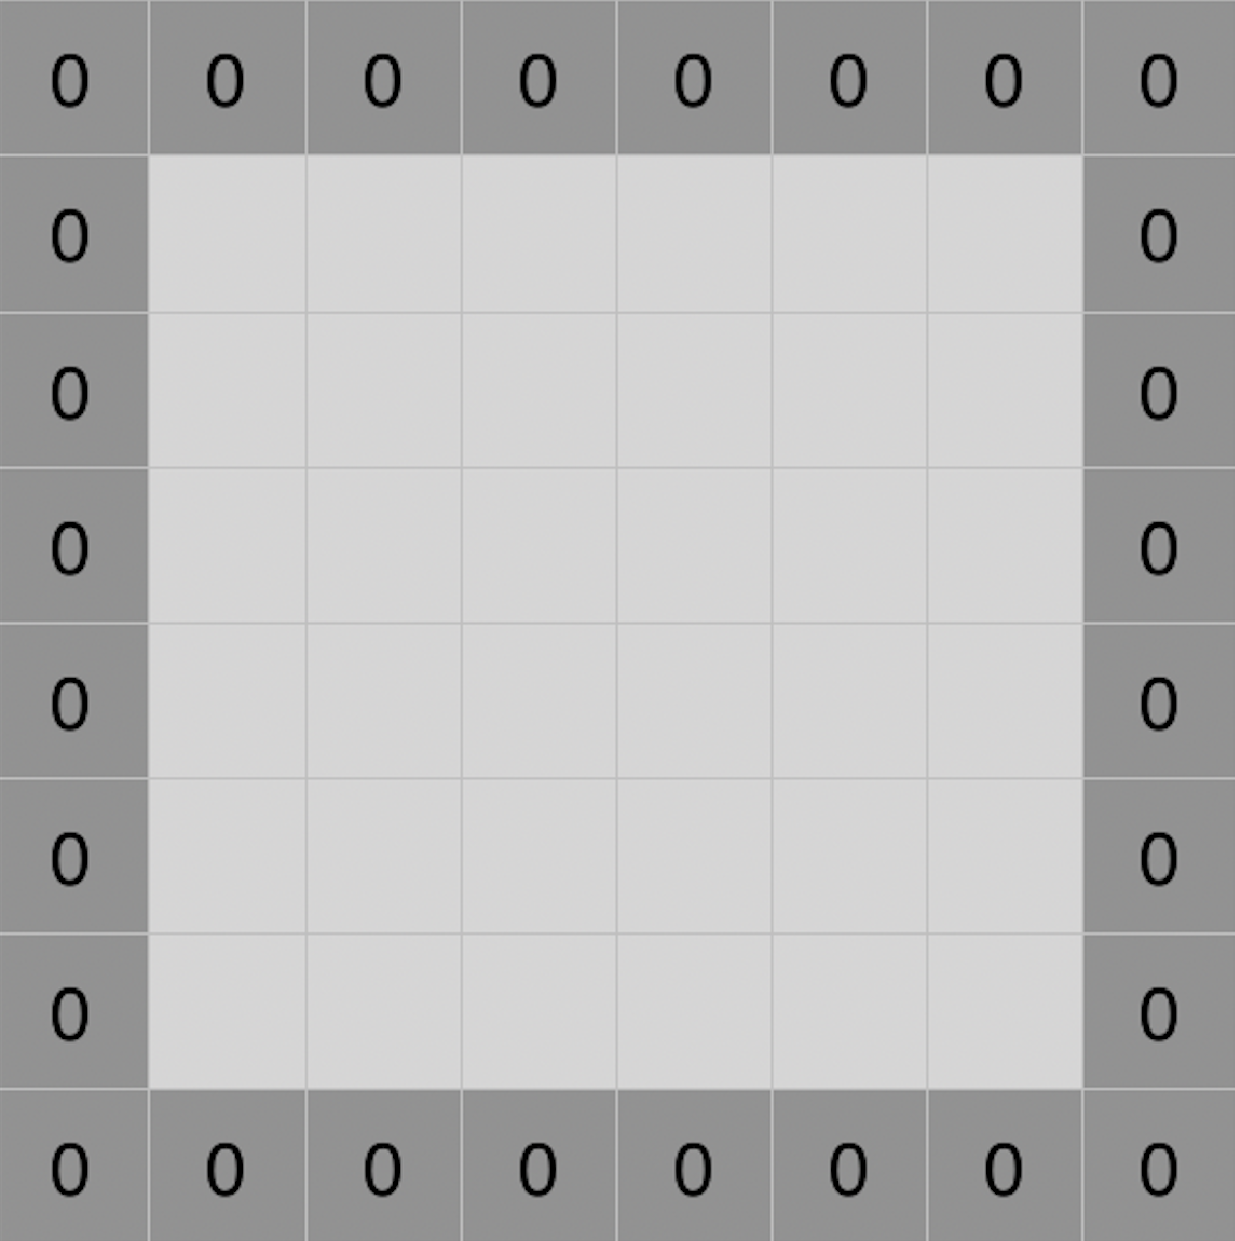
\includegraphics[width=0.2\textwidth]{zeropadding.pdf}
\caption{Example of Zero-padding Added to Image \cite{pooling}}
\label{fig:padding}
\end{figure}

%pooling
\paragraph{Pooling}
After the convolution operation, we extracted a lot of feature information. Adjacent areas have similar feature information and can be replaced with each other. If all these feature information are retained, there will be information redundancy, which increases the computational difficulty. At this time, pooling is equivalent to a dimension reducing operation. 

Pooling happens in a small matrix area. The maximum or average value of the area will be used to replace the area. The size of the small matrix can be set when the network is built. This small matrix is scanning from the upper left corner to the lower right corner when perform pooling.

\begin{figure}[h!]
\centering
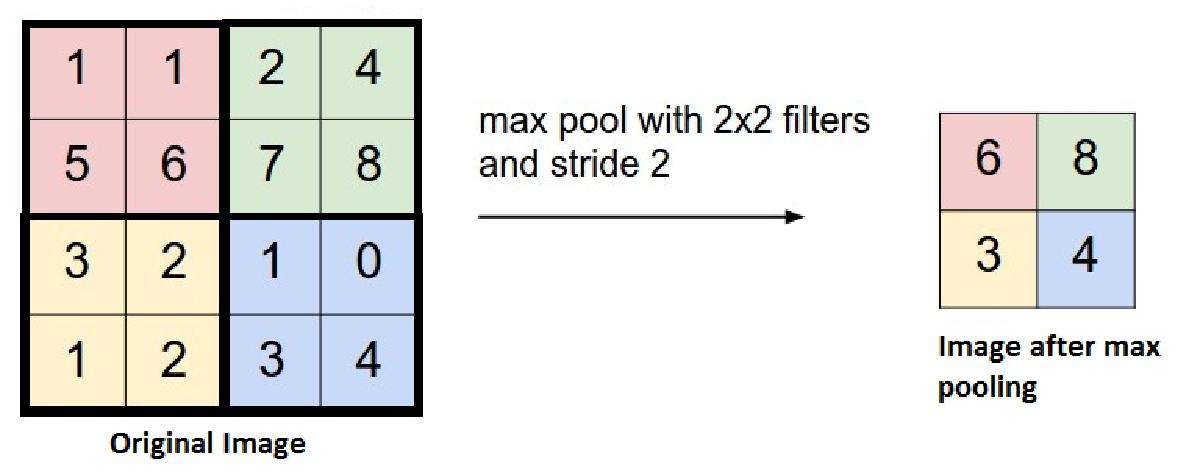
\includegraphics[width=0.65\textwidth]{pooling.pdf}
\caption{Example of Max-pooling \cite{pooling}}
\label{fig:pooling}
\end{figure}

\paragraph{Fully Connected Layer}
%fully connected layers
For layers $n-1$ and $n$, any node in layer $n-1$ is connected to all nodes in layer $n$. That is, when each node of the $n$-th layer performs calculations, the input of the activation function is the weight of all nodes of the $n-1$ layer. The middle layer like below is fully connected.

\begin{figure}[h!]
\centering
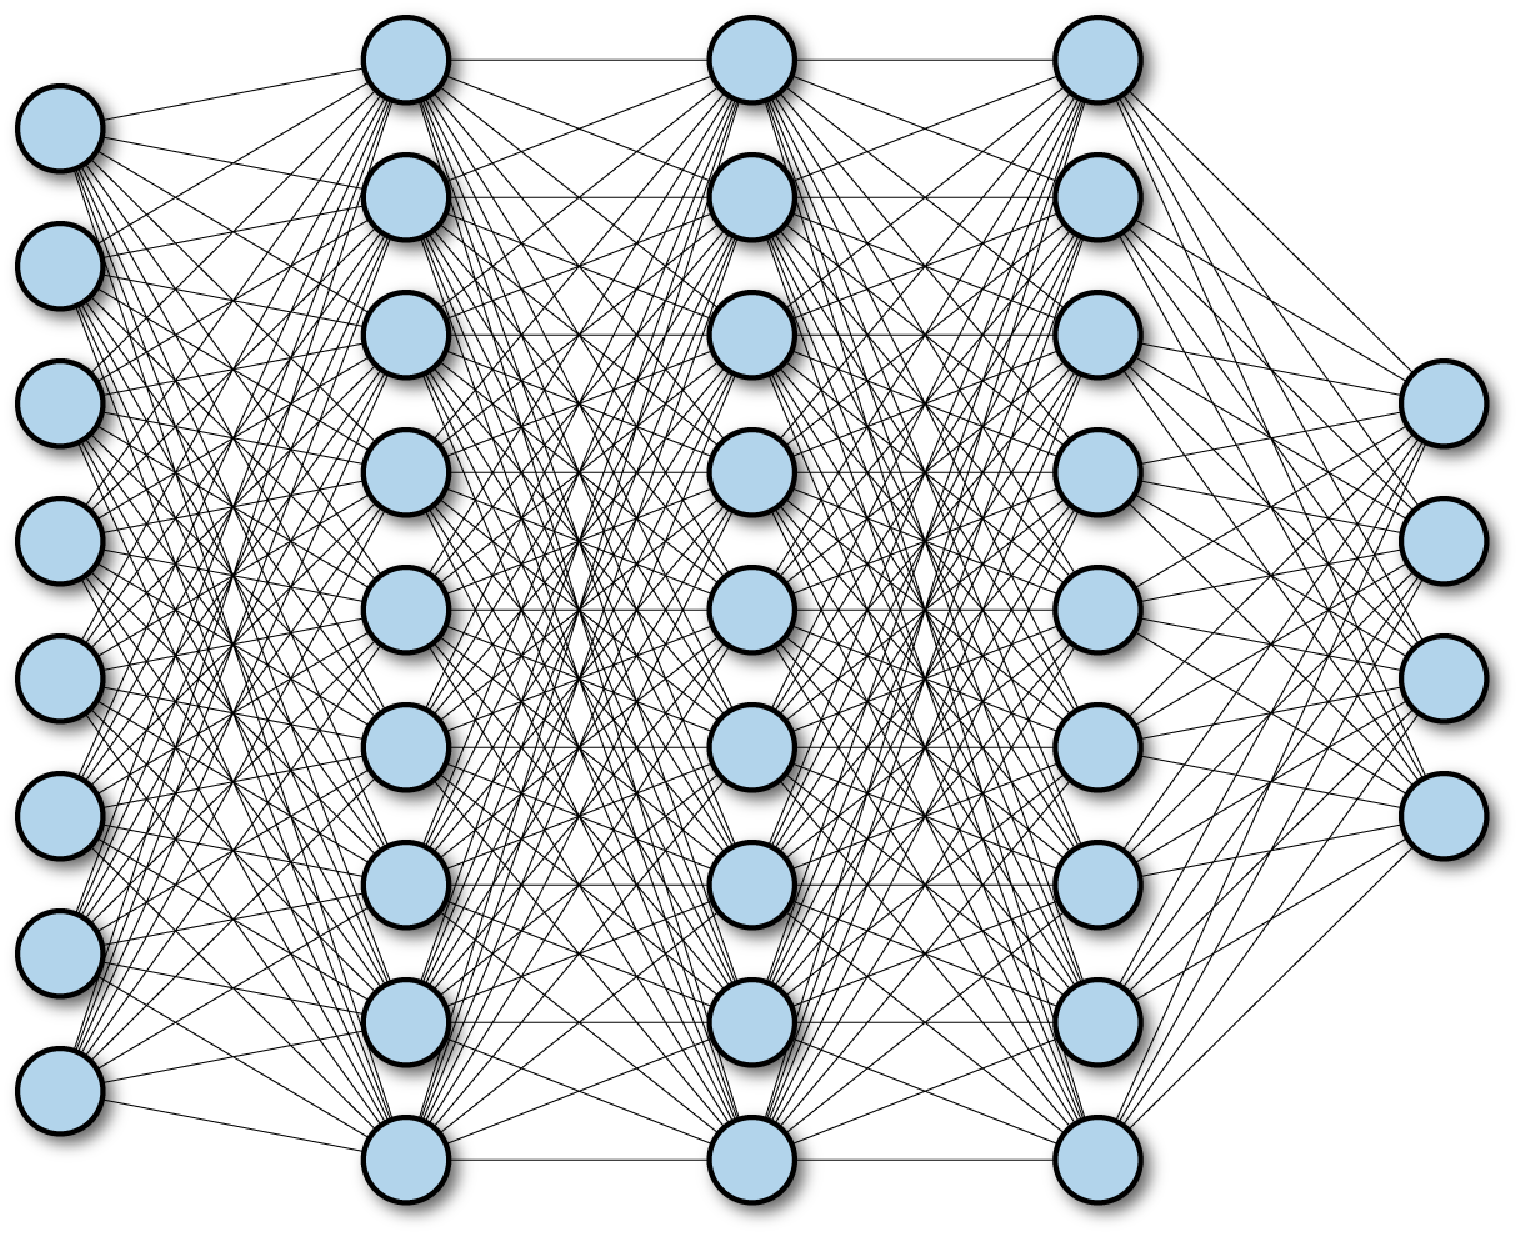
\includegraphics[width=0.5\textwidth]{fullyconnected.pdf}
\caption{Example of Fully Connected Layer}
\label{fig:fully}
\end{figure}

\subsubsection{VGG16}

\verb|VGG16| \cite{vgg16} is a deep network model developed by the computer vision team of Oxford University and researchers at Google DeepMind in 2014. The network has a total of 16 training parameters. The \verb|VGG16| network won the second place in the ILSVRC 2014 competition classification project and the first place in the positioning project, which proved its asset and made it a very commonly used model in the field of CNN.

\paragraph{Configuration}
\verb|VGG| has a relatively simple structure, and its generalisation performance of migrating to other image also achieves well. \verb|VGG| is still often used to extract image features.

According to the different sizes of the convolution kernel and the numbers of convolution layers in VGG, it can be divided into 6 ConvNet configuration: \verb|A|, \verb|A-LRN|, \verb|B|, \verb|C|, \verb|D|, \verb|E|, of which \verb|D| and \verb|E| are more commonly used, which are called \verb|VGG16| and \verb|VGG19| respectively. The following Figure \ref{fig:vgg16config} shows the six structural configurations of VGG. In Figure \ref{fig:vgg16config}, each column corresponds to a structural configuration. For example, section \verb|D| in the figure indicates the structure adopted by \verb|VGG16|.

\begin{figure}[h!]
\centering
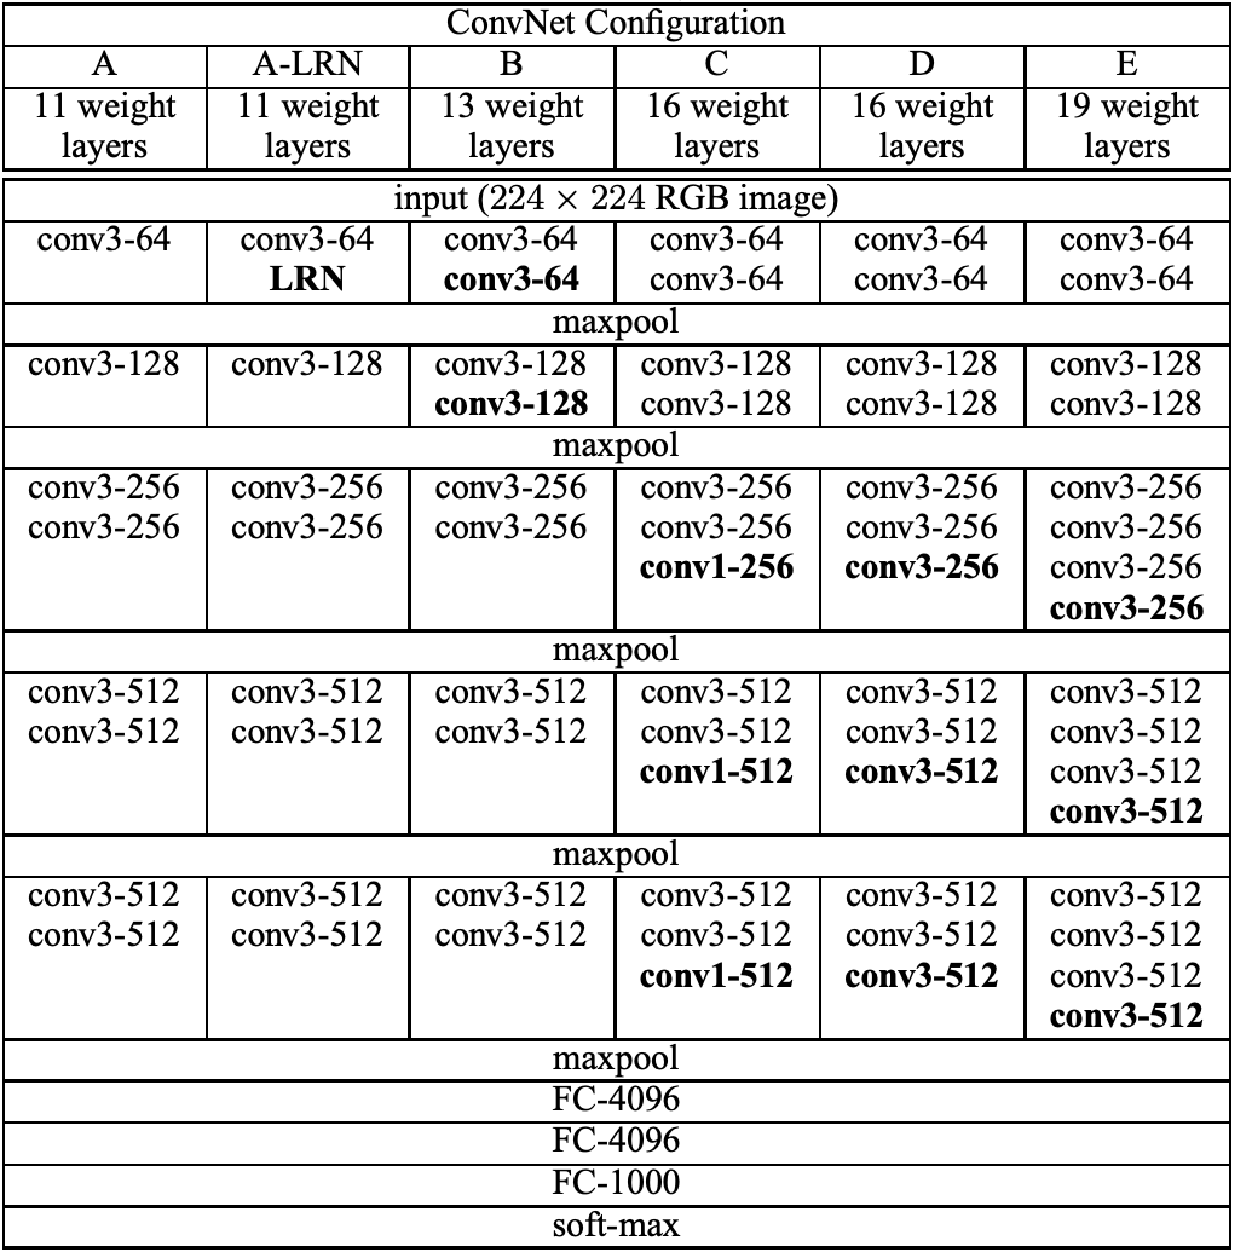
\includegraphics[width=0.7\textwidth]{vgg.pdf}
\caption{ConvNet Configuration of VGG \cite{vgg16}}
\label{fig:vgg16config}
\end{figure}

\verb|VGG16| contains the following components:
\begin{itemize}
    \item 13 Convolutional Layers, each represented by \verb|conv3-XXX|
    \item 3 Fully connected Layers, each represented by \verb|FC-XXXX|
    \item 5 Pool layers, each represented by \verb|maxpool|
\end{itemize}

Among them, the convolutional layer and the fully connected layer have weight coefficients, so they are also called weight layers. The total number is $13+3=16$, which is the source of 16 in \verb|VGG16|. (The pooling layer does not involve weights, so it does not belong to the weighting layer and is not counted).

%features
\paragraph{Structure and Features}
The outstanding feature of \verb|VGG16| is simplicity, which is reflected in:

\begin{itemize}
    \item The convolutional layers all use the same convolution kernel parameters.
    \item The convolution layers are all represented as \verb|conv3-XXX|, where \verb|conv3| indicates that the size of the convolution kernel is 3, that is, the width and height are both 3. And $3\times3$ is very small kernel size, combined with other parameters: \verb|stride = 1|, \verb|padding = same|, so that each convolutional layer (tensor) can maintain the same width and high. \verb|XXX| represents the number of channels of the convolutional layer.
    \item The pooling layer uses the same pooling kernel parameters. 
    \item The model is composed of several convolutional layers and pooling layers stacked, which is relatively easy to form a deeper network structure (considering that back to 2014, 16 layers have been considered very deep).
    
\end{itemize}

Based on the above analysis, the advantages of \verb|VGG16| can be summarised as: small filters and deeper networks.

Figure \ref{fig:vgg16strucure} illustrates the overall structure of \verb|VGG16|. From left to right, a coloured picture is the input to the network. The white box is the convolution layer, the red is the pooling, the blue is the fully connected layer, and the brown box is the prediction layer. The role of the prediction layer is to convert the information output from the fully connected layer into the corresponding class probability, and play a classification role.

\begin{figure}[h!]
\centering
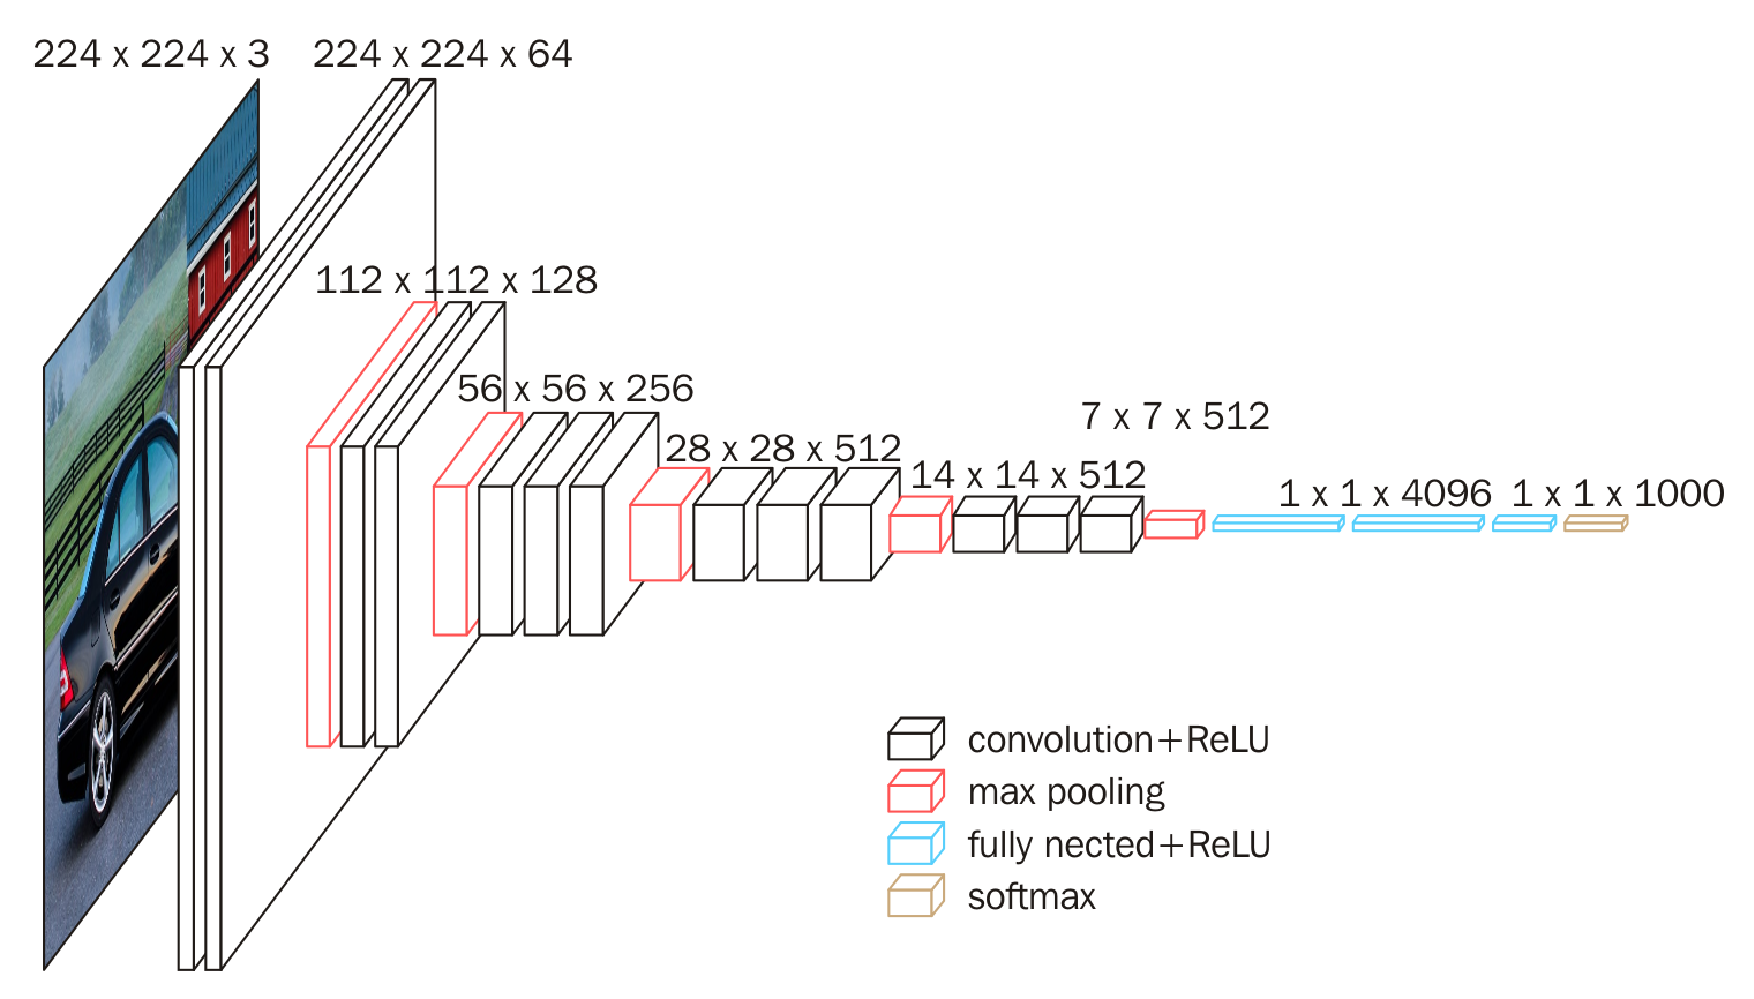
\includegraphics[width=1\textwidth]{vgg16struc.pdf}
\caption{General Structure of VGG16 Model \cite{vgg16}}
\label{fig:vgg16strucure}
\end{figure}

%block structure
\paragraph{Block Structure}
We note that on the right side of Figure \ref{fig:vgg16strucure}, the convolutional layer and pooling layer of \verb|VGG16| can be divided into different blocks, which are numbered \verb|Block1| to \verb|block5| from front to back. Each block contains several convolutional layers and a pooling layer. For example: \verb|Block4| contains:
\begin{itemize}
    \item 3 convolutional layers: \verb|conv3-512|
    \item 1 pooling layer: \verb|maxpool|
\end{itemize}

And in the same block, the number of channels of the convolutional layer is the same, for example:
\begin{itemize}
    \item \verb|block2| contains 2 convolutional layers, each of which is represented by \verb|conv3-128|, that is, the convolution kernel is: $3\times3\times3$, the number of channels is 128
    \item \verb|block3| contains 3 convolution layers, each convolution layer is represented by \verb|conv3-256|, that is, the convolution kernel is: $3\times3\times3$, the number of channels is 256
\end{itemize}

The structure of \verb|VGG16| divided by blocks is given below in Figure \ref{fig:vgg16blockstrucure}.

\begin{figure}[h!]
\centering
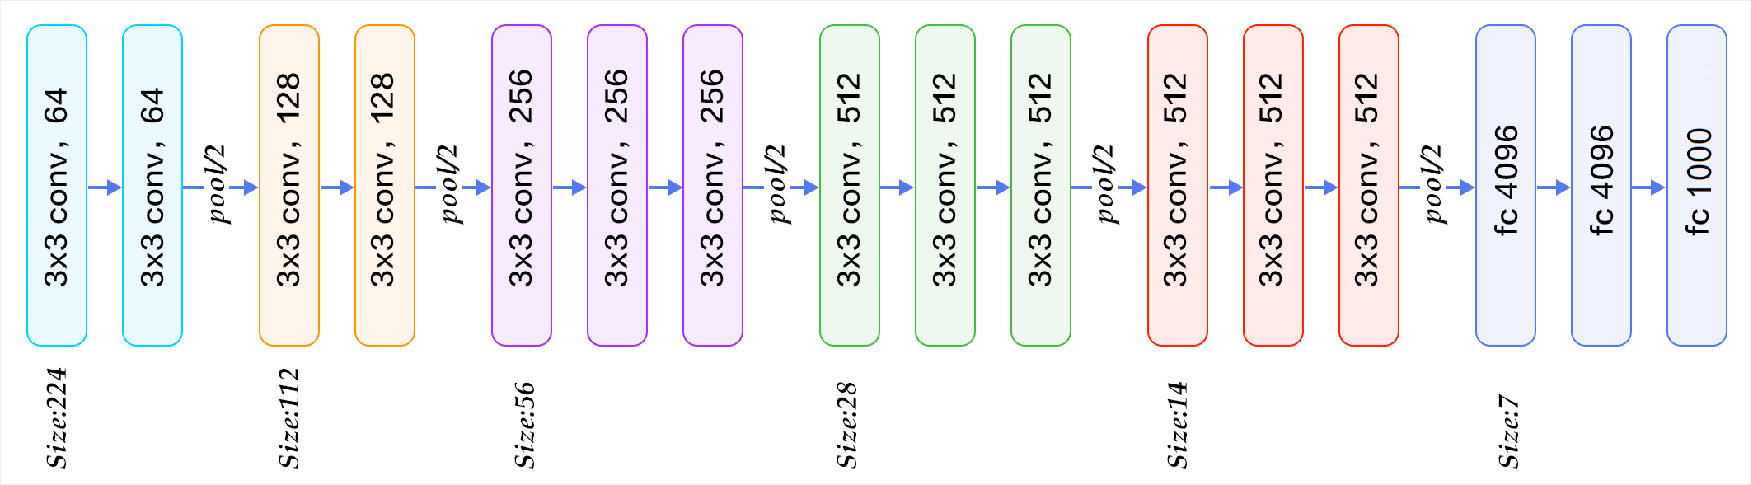
\includegraphics[width=.9\textwidth]{vgg16blockstruc.pdf}
\caption{Structure of VGG16 Model by Blocks \cite{vgg16}}
\label{fig:vgg16blockstrucure}
\end{figure}

The input image of \verb|VGG| is $224\times224\times3$:
\begin{itemize}
    \item The number of channels doubles, from 64 to 128 in order, and then to 256, until 512 remains the same and no longer doubles
    \item Height and width change halved from $224 \to 112 \to 56 \to 28 \to 14 \to 7$
\end{itemize}

\subsubsection{2-stage Model}

The 2-stage model is named for its 2-stage processing of pictures, also known as the region-based method. Here we choose the R-CNN series work as a representative of 2-stage model, which is also the model we adopted for this project.

\subsubsection{R-CNN}
Traditional computer vision methods often use well-designed manual features, such as SIFT and HOG to describe images, while deep learning methods advocate the acquisition of features. From the experience of image classification tasks, the effects obtained by the CNN network automatically acquired features has exceeded the characteristics of manual design. Girshick et al. \cite{rcnn} applied convolutional networks in local areas to give convolutional networks ability to learn high-quality features.

R-CNN abstracts detection into two processes. One is to propose some regions that may contain objects based on the picture, that is, the local cropping of the picture, called the ``Region Proposal''. The paper \cite{rcnn} used the Selective Search algorithm then run the best performing classification network, i.e. AlexNet on the areas, and then obtained the categories of objects in each area. A basic structure of R-CNN is illustrated below as Figure \ref{fig:rcnn}.

\begin{figure}[h!]
\centering
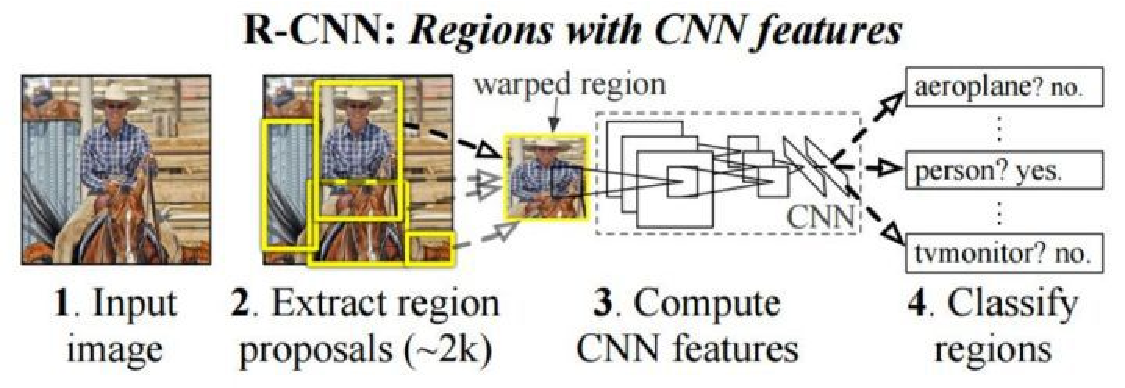
\includegraphics[width=0.7\textwidth]{rcnn.pdf}
\caption{Structure of R-CNN \cite{rcnn}}
\label{fig:rcnn}
\end{figure}

The proposal of R-CNN has two significant contributions: first, CNN can be used for region-based localisation and segmentation of objects; second, when the number of supervised training samples is scarce, pre-trained models on additional data can achieve excellent results after fine-tuning. The first contribution motivated almost all 2-stage methods, and the second contribution used the model trained in the classification task (Imagenet \cite{imagenet}) as the base network. The fine-tuning method for detecting problems has also been used widely in the subsequent works.

The idea of R-CNN is straightforward, the detection task is transformed into a classification task on the region, which is a test of the deep learning method on the detection task. There are also many issues with the model itself, such as the need to train three different models: proposal, classification, regression and performance problems caused by repeated calculations, etc. But R-CNN can still be considered as the pioneer ``the first paper'' in the field.

\subsubsection{Fast R-CNN}
In 2015 Girshick \cite{fastrcnn} pointed out the reason why R-CNN is time-consuming is that CNN is performed separately on each Proposal. Without sharing calculations, it is proposed that after the basic network is run on the entire picture, it is introduced into the R-CNN sub-network, sharing the large Partially calculated, hence the name ``Fast''.

\begin{figure}[h!]
\centering
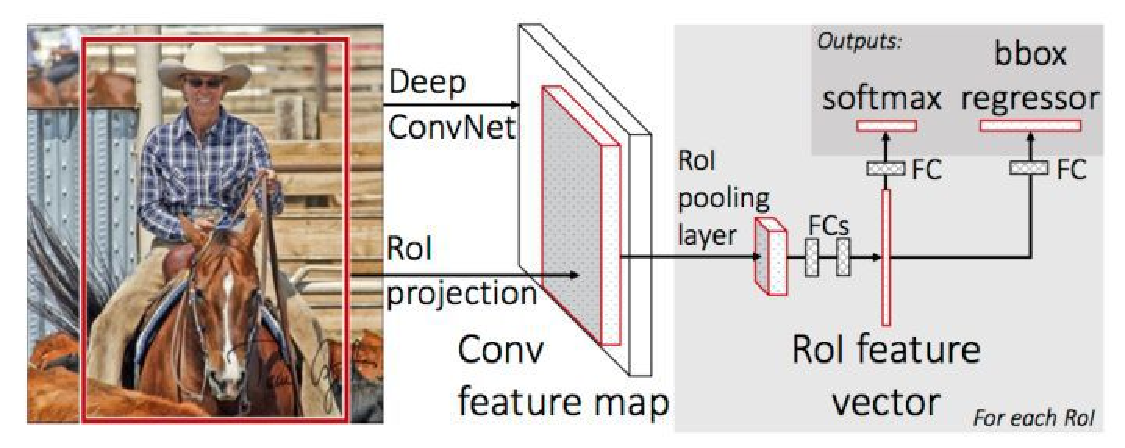
\includegraphics[width=0.7\textwidth]{fastrcnn.pdf}
\caption{Structure of Fast R-CNN \cite{fastrcnn}}
\label{fig:fastrcnn}
\end{figure}

Figure \ref{fig:fastrcnn} above shows the architecture of Fast R-CNN. A feature map is obtained from the feature extractor, at the same time, a Selective Search algorithm is run on the original image and the RoI i.e. Region of Interset, a coordinate group that can be mixed with Region Proposal is mapped to the feature map. Then RoI Pooling is performed for each RoI, this operation obtains feature vectors of equal length, then sorts the obtained feature vectors into positive and negative samples when maintains a certain ratio of positive and negative samples. Next Fast R-CNN batches them into the parallel R-CNN sub-network, performs classification and regression at the same time and unify both losses.

This structure of Fast R-CNN is exactly the prototype of the meta-structure adopted by the mainstream 2-stage method for detection tasks. Fast R-CNN \cite{fastrcnn} unifies Proposal, Feature Extractor, Object Classification and Localisation in a whole structure, and improves the efficiency of feature utilisation through shared convolution calculations, which is the most contributing content.

\subsubsection{Faster R-CNN}
\label{sec:fasterrcnn}
Faster R-CNN \cite{fasterrcnn} is the foundation work of the 2-stage method. The proposed RPN network replaces the Selective Search algorithm so that the detection task can be completed end-to-end by the neural network. Roughly speaking, Faster R-CNN is a combination of RPN plus Fast R-CNN, sharing the characteristics of convolution calculation with RCNN makes the calculation brought by RPN relatively small, so Faster R-CNN can run at 5fps on a single GPU and reaches SOTA in terms of accuracy.

The main contribution of Faster R-CNN \cite{fasterrcnn} is the proposal of Regional Proposal Networks to replace the previous SS algorithm. RPN network models the task of Proposal to the problem of binary classification: whether it is an object. Figure \ref{fig:fasterrcnn} below illustrate the basic structure of Faster R-CNN \cite{fasterrcnn}.

\begin{figure}[h!]
\centering
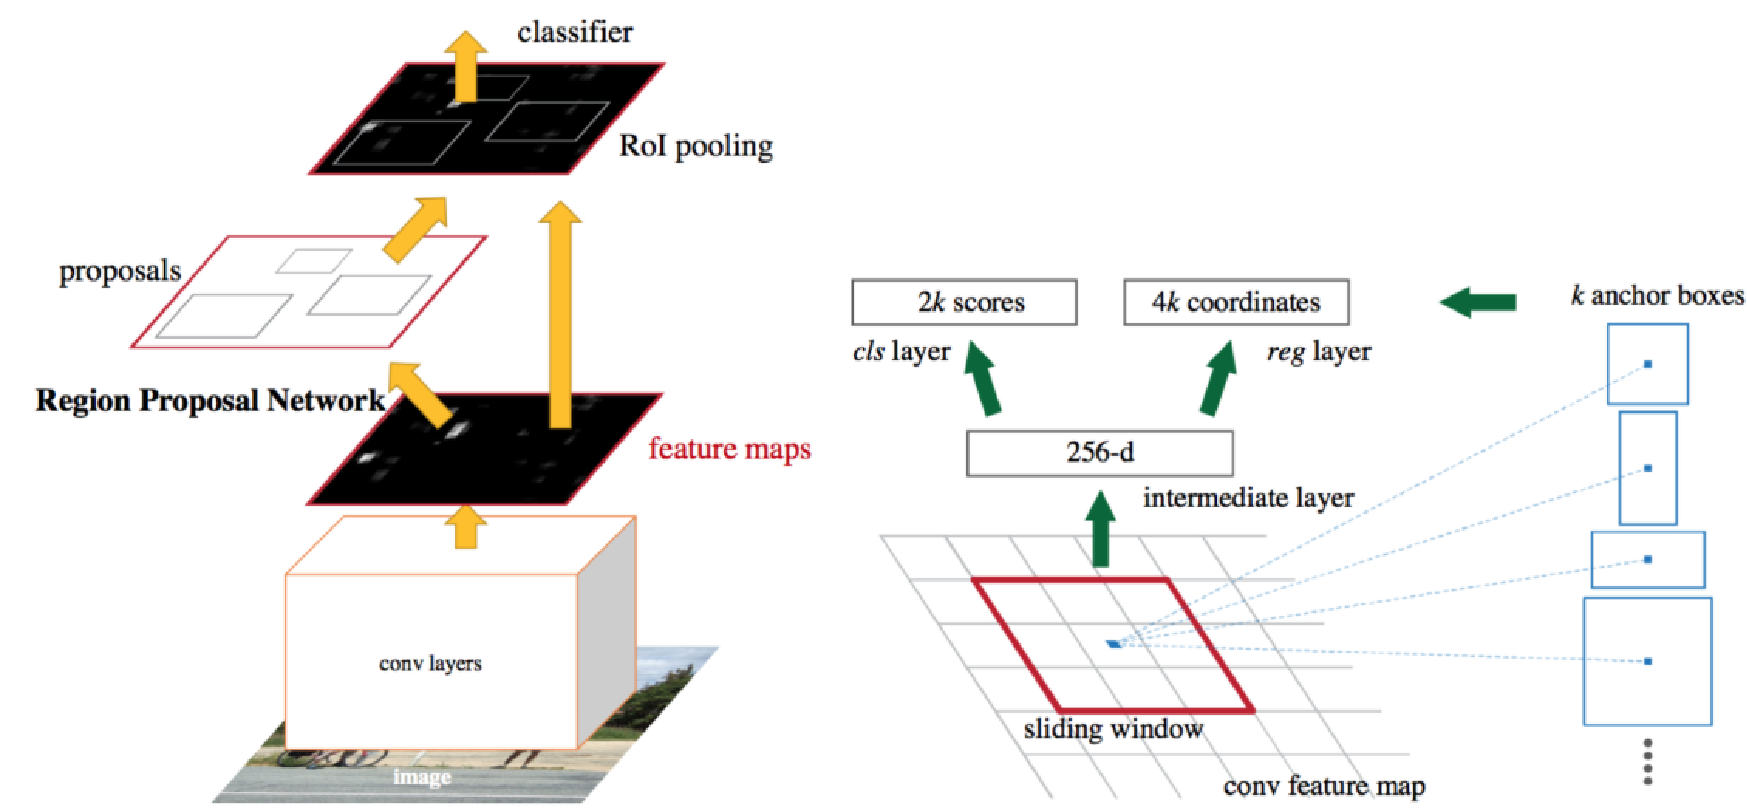
\includegraphics[width=0.8\textwidth]{fasterrcnn.pdf}
\caption{Structure of Faster R-CNN \cite{fasterrcnn}}
\label{fig:fasterrcnn}
\end{figure}

The first step is to generate anchor boxes with various size and aspect ratio on a sliding window (as shown in the right part of Figure \ref{fig:fasterrcnn}), give IoU a predetermined threshold, label anchor box as positive or negative corresponding to the Ground Truth. Thus, the input samples to RPN is organised into anchor box (coordinates) of each anchor box and whether this anchor box has an object or not (binary label). RPN network maps each sample to four coordinate values and a probability value which corresponds the probability of there is an object in the anchor box, values for the four coordinates define the position of the object. Finally, combine the loss of binary and coordinate regression, as the target of training RPN network.

Faster R-CNN completed the ``deep'' part of the inspection tasks using RPN network. The idea of using a sliding window to generate anchor box is also widely adopted such as in YOLO v2, etc. 


\section{Image-text Alignment}
Image-text matching and visual question answering (VQA) are the frontiers of image and text multi modal fusion. The former needs to map images and texts to the same semantic space, and then judge their similarity by distance; the latter needs to find suitable answers in all candidate sets.

\subsection{Convolutional Neural Network Architectures for Matching Natural Language Sentences}

This paper \cite{hu2015convolutional} is a common method for text processing used in Image-Text Matching tasks, which is equivalent to a classic work of natural language processing.

The core idea is to apply the convolution operation to text. The problem to be solved in this article is the matching between Text.

\subsubsection{Text Convolutional}
First of all, we explain the convolution operation of the text. After the discrete text information: embedding is done, the continuous features of the text will be obtained, that is, a word can be represented by a vector. At this time, it is very similar to process an image. A word is equivalent to one pixel in an image, and a sentence is composed of several such words. In a specific implementation, the feature dimension of Embedding can be equivalent to the number of channels in the image, so that the words are connected end to end, and an image with a length of $1\times N$ (the number of text words) is finally formed. At this time, a convolutional network of text can be implemented.

Images can be resized to the same size by linear transformation methods, but text cannot, so the convolution of the text generally uses a Gated Convolutional Layer, that is, for sentences of insufficient length, it is forced to zero, as shown below in Figure \ref{fig:cnnamnls1}:

\begin{figure}[h!]
\centering
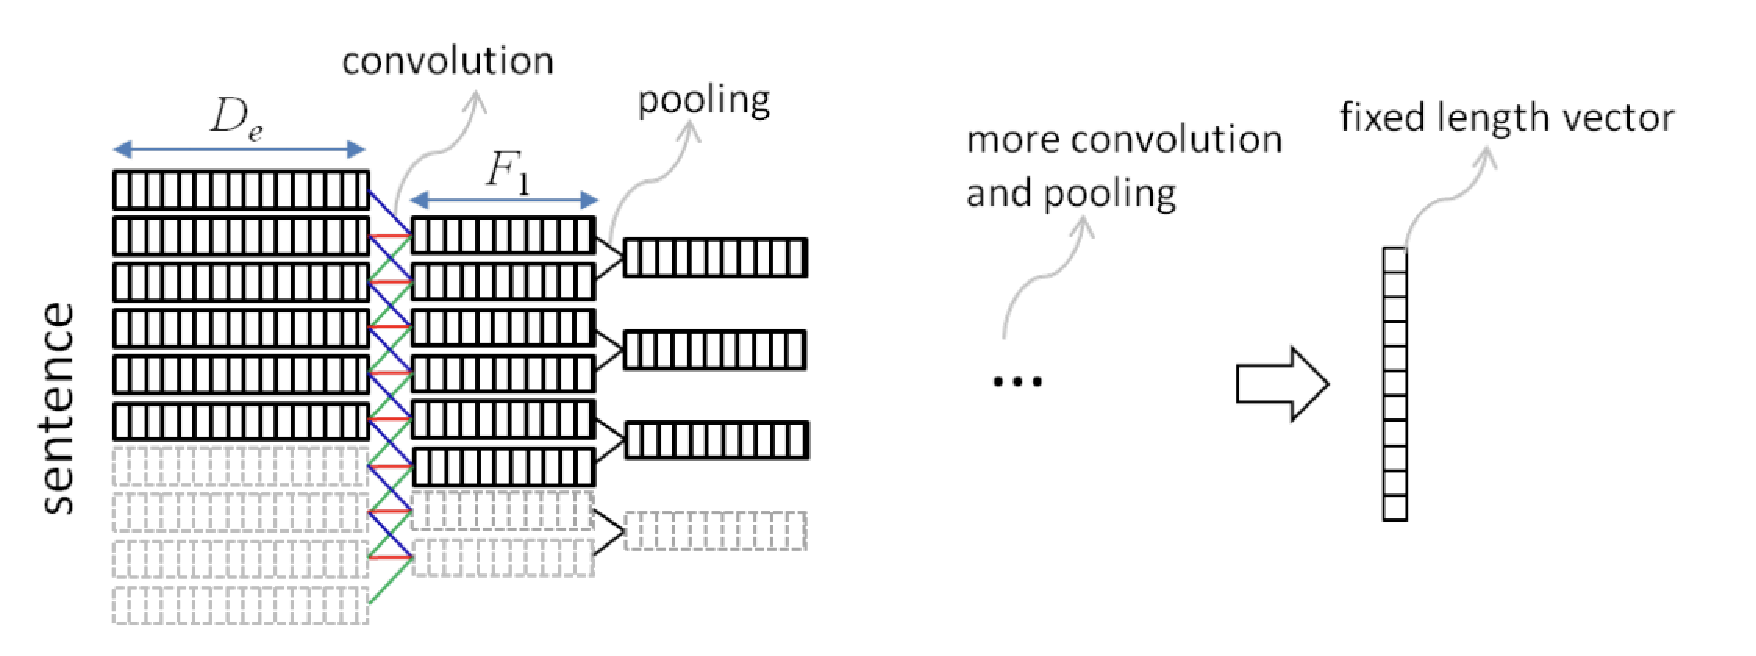
\includegraphics[width=.8\textwidth]{cnnamnls1.pdf}
\caption{Structure of Convolutional Sentence Model \cite{hu2015convolutional}}
\label{fig:cnnamnls1}
\end{figure}

Another point to note is that Maxpooling will be selected as the pooling method for general text so that local features can be maximised accordingly.

\subsubsection{Architecture}
This paper proposed two network structures. One is the matching post-fusion technology, that is, to obtain their vector representation through CNN in two texts to be matched, and then perform stitching and add several layers of full connections to predict the final match.

The network structure of Arc-I is shown in the Figure \ref{fig:cnnamnls2}:

\begin{figure}[h!]
\centering
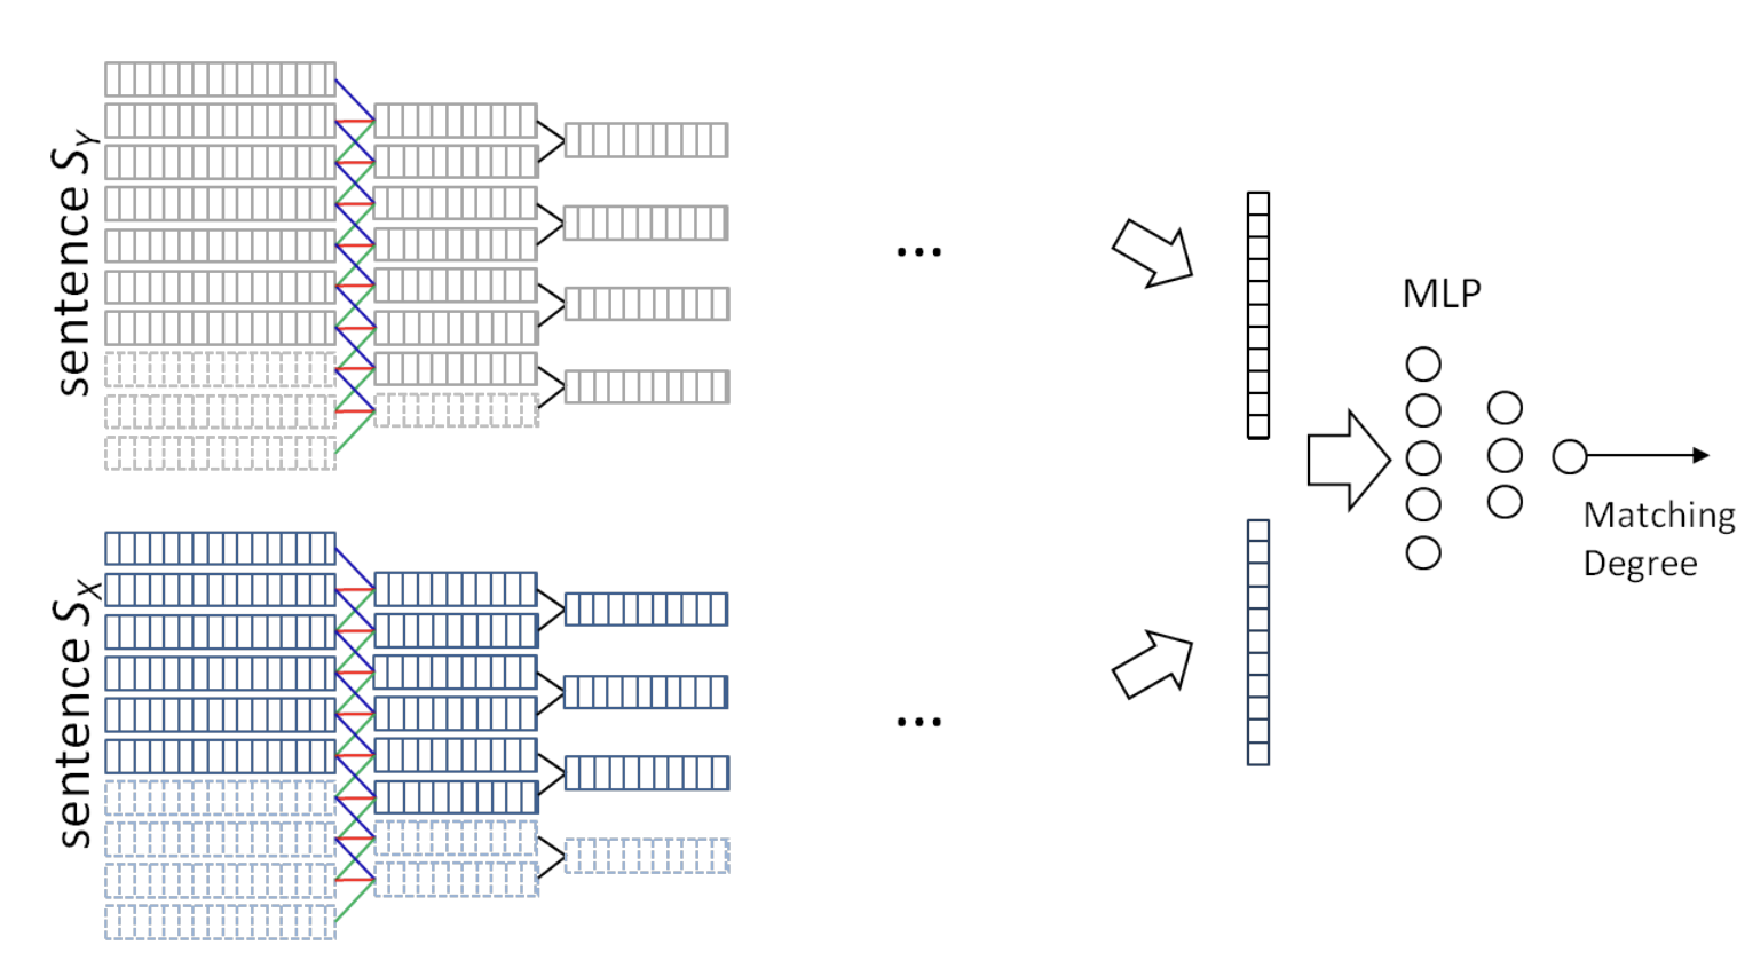
\includegraphics[width=.8\textwidth]{cnnamnls2.pdf}
\caption{Arc-I for matching two sentences \cite{hu2015convolutional}}
\label{fig:cnnamnls2}
\end{figure}

It can be seen from the figure that its feature processing method of encoding belongs to the post-fusion of features, and is very naive. In such a network model, the author did not consider the correlation between different sentences and the order of words, that is, the model mapped the two sentences into a semantic space involuntarily. In order to solve this problem, the author developed a second method:

The network structure of Arc-II is shown in the Figure \ref{fig:cnnamnls3}:

\begin{figure}[h!]
\centering
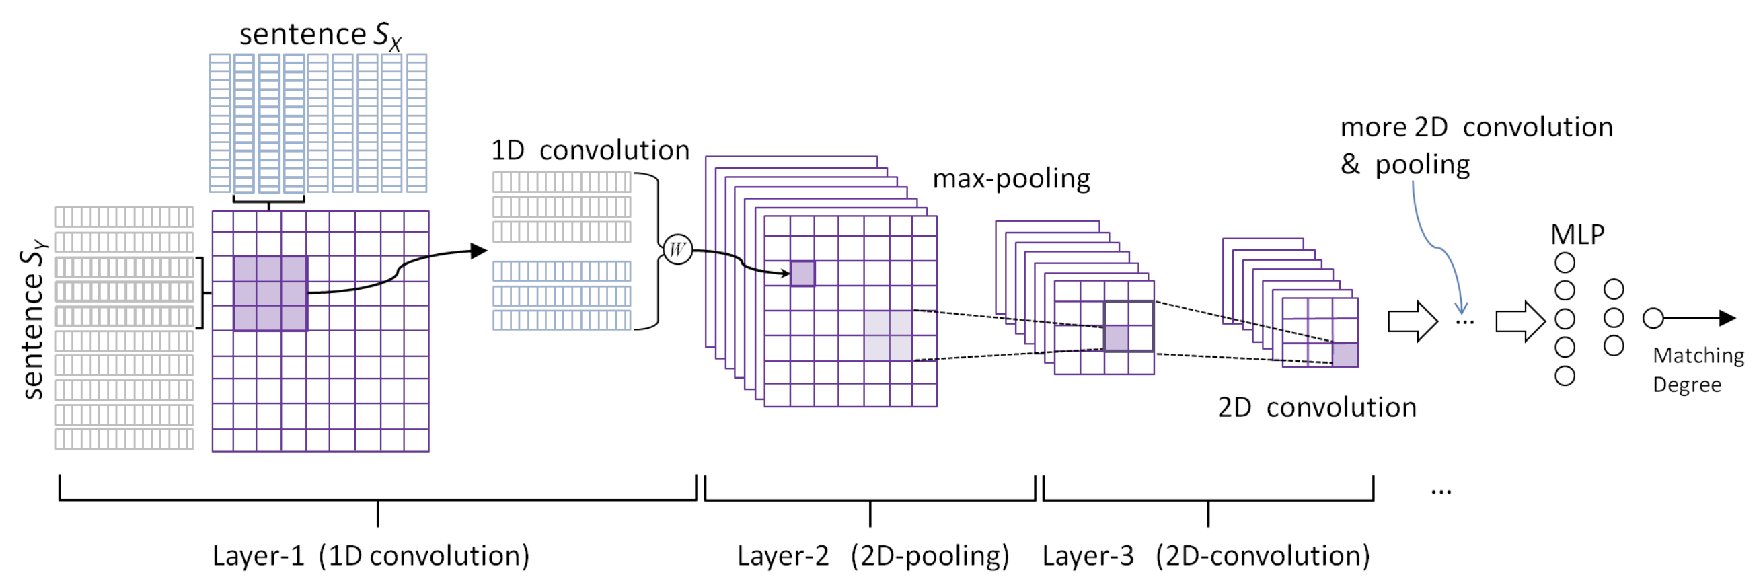
\includegraphics[width=\textwidth]{cnnamnls3.pdf}
\caption{Arc-II of convolutional matching model \cite{hu2015convolutional}}
\label{fig:cnnamnls3}
\end{figure}

This model combined all the word positions of the two sentences, and each position was expressed by the following formula:

$$
\hat{\mathbf{z}}_{i, j}^{(0)}=\left[\mathbf{x}_{i: i+k_{1}-1}^{\top}, \quad \mathbf{y}_{j: j+k_{1}-1}^{\top}\right]^{\top}
$$

$x$ and $y$ respectively represent the sentence to be matched. According to the above formula, the two sentences will form a square \verb|FM1|. Each position of \verb|FM1| is composed of $2k_1$ vectors. That is, this is actually a 4-dimensional structure \verb|[#Sentence * #Sentence * 6 * #Embd_size]|. A one-dimensional convolution using the latter two dimensions will form a three-dimensional feature map of \verb|layer-2|.

Then the network structure behind is the common model in the image.

\subsubsection{Summary}
\begin{itemize}
    \item The convolutional network processes text data and introduces location information into the convolutional network to form a 3d feature map. Gated Convolution, to ensure that the gradient will not be affected when the sentence is not long enough.
    \item MaxPooling guarantees maximum response of local features.
\end{itemize}

\subsection{m-CNNs}

This work \cite{ma2015multimodal} needs to solve the problem of image and text matching. There is not much innovation in image features, that is, features extracted by CNN networks. Different from his previous work, it fuses image features with text features and directly inputs them to the convolutional network for matching. m-CNNs also pays attention to text information with different granularities.

The way m-CNNs deals with features is by directly concatenating the features.

\subsubsection{Word-level Matching CNN}
The finest-grained matching problem. The network structure is as follows:

\begin{figure}[h!]
\centering
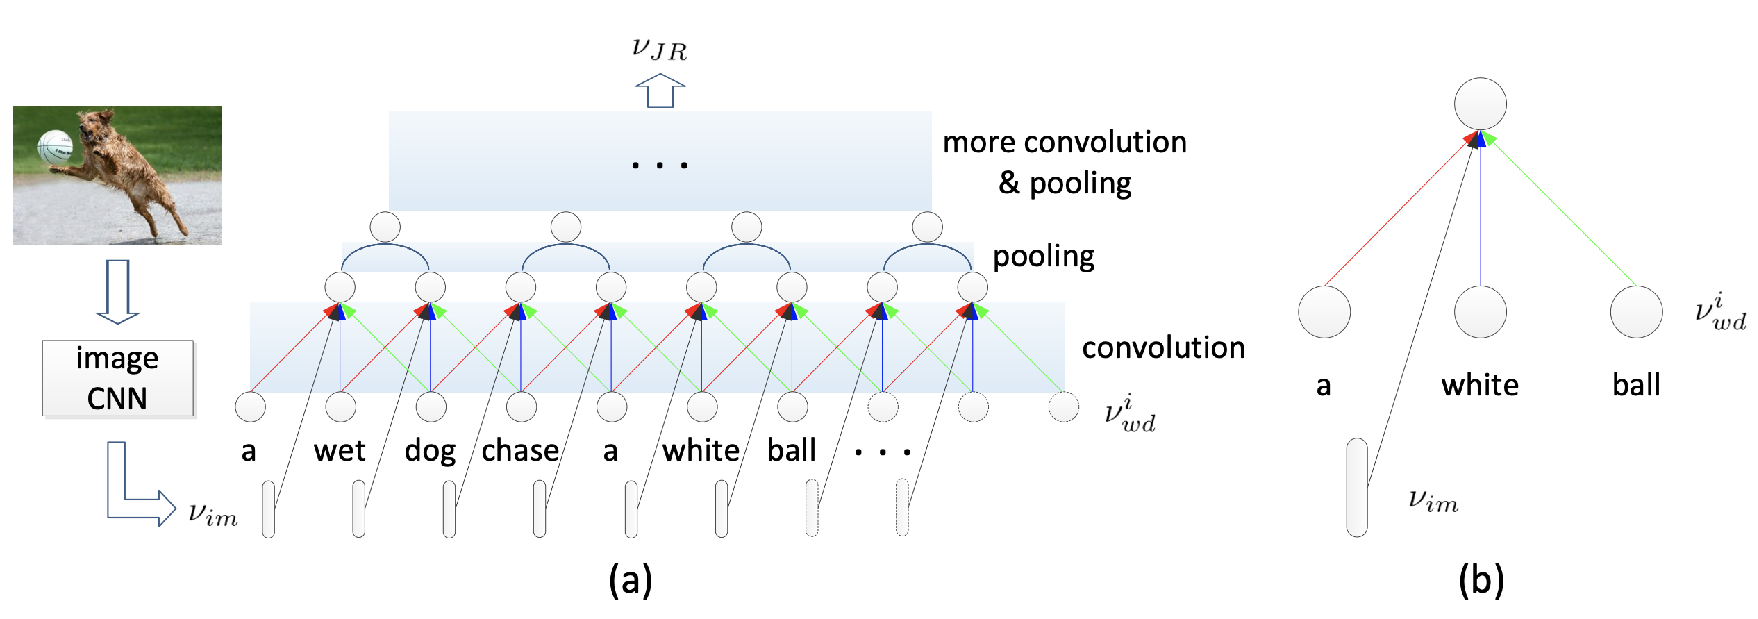
\includegraphics[width=\textwidth]{mccns1.pdf}
\caption{The word-level matching CNN. \cite{ma2015multimodal}}
\label{fig:mccns1}
\end{figure}

The calculation formula is as follows:

$$
\vec{\nu}_{(0)}^{i} \stackrel{\text { def }}{=} \nu_{w d}^{i}\left\|\nu_{w d}^{i+1}\right\| \cdots\left\|\nu_{w d}^{i+k_{r p}-1}\right\| \nu_{i m}
$$

\subsubsection{Phase-level Matching CNN}
Word granularity matching, the network structure is as follows:

\begin{figure}[h!]
\centering
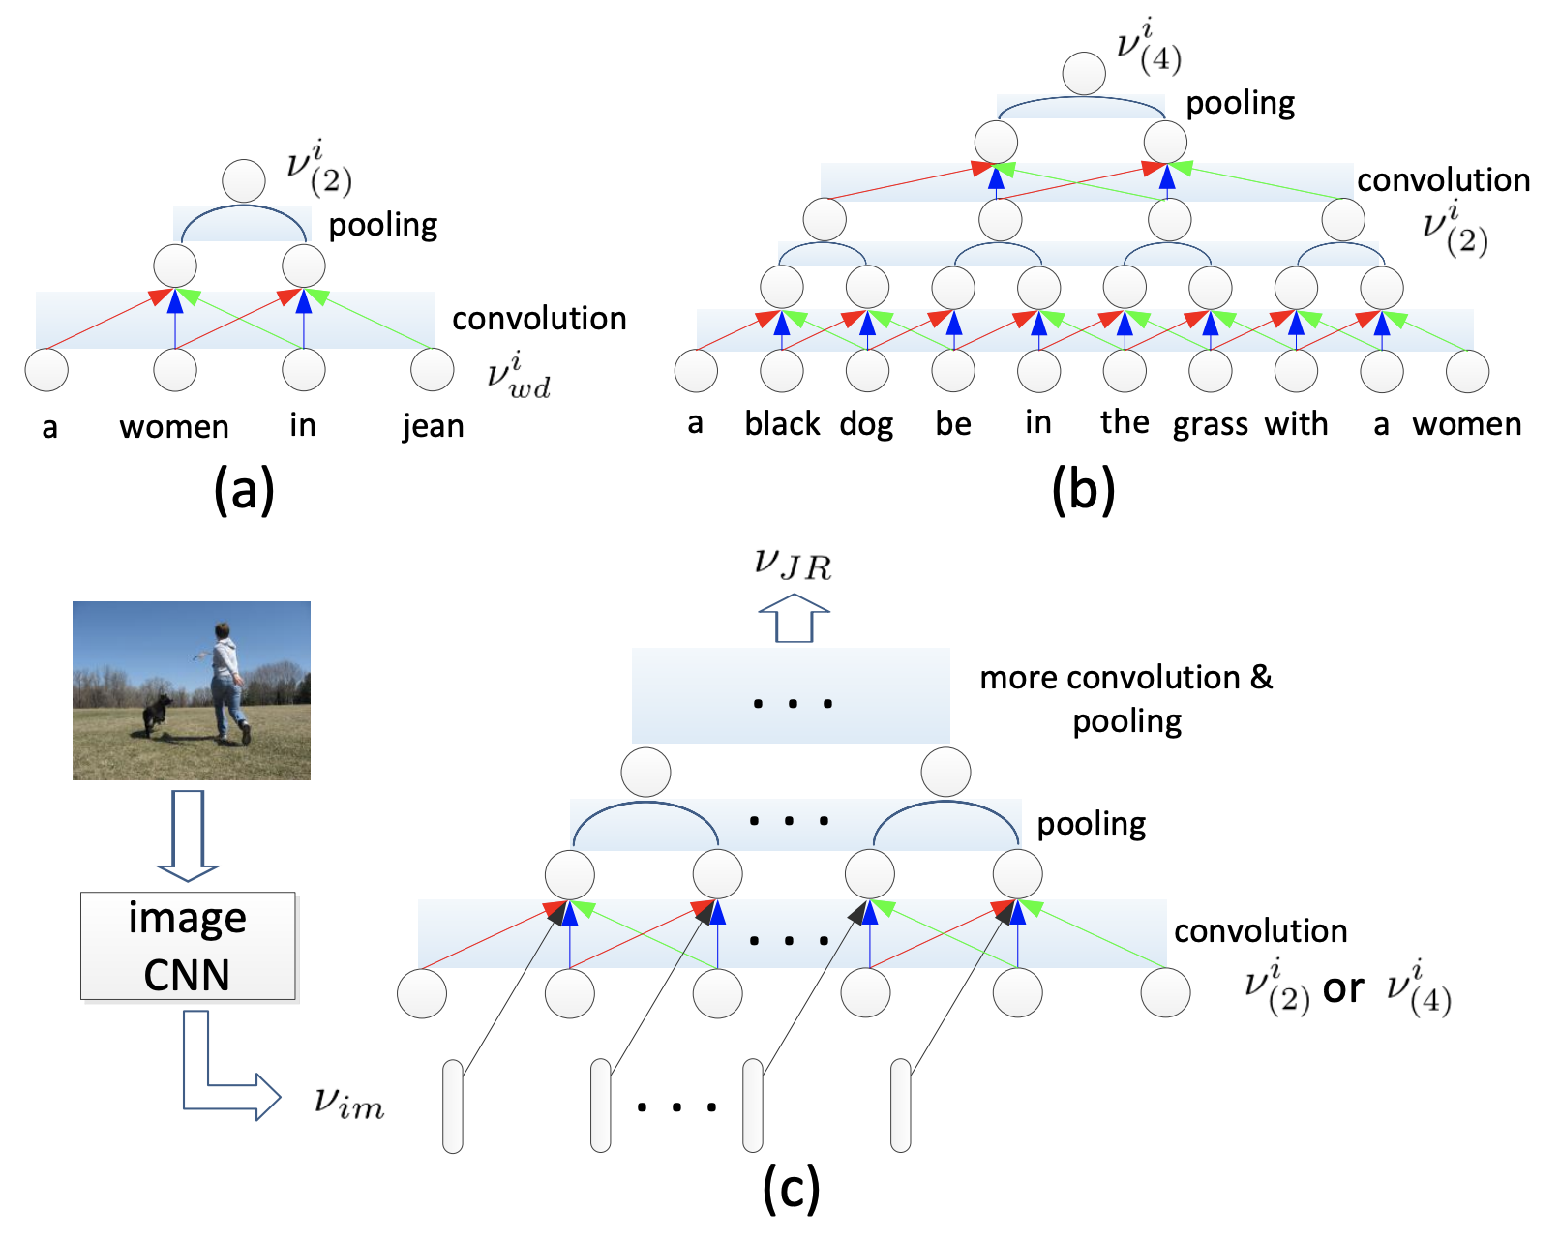
\includegraphics[width=\textwidth]{mccns2.pdf}
\caption{ The phrase-level matching CNN and composed phrases. \cite{ma2015multimodal}}
\label{fig:mccns2}
\end{figure}

The calculation formula is as follows:
$$
\vec{\nu}_{p h}^{i} \stackrel{\text { def }}{=} \nu_{p h}^{i}\left\|\nu_{p h}^{i+1}\right\| \cdots\left\|\nu_{p h}^{i+k_{r p}-1}\right\| \nu_{i m}
$$

Phrase-level matching CNN is similar to word, except that the position is different. The author uses two different granularity phrases in the text, one is two words and one is four words.

A very useful concept in this is the receptive field, which means that a neuron is calculated from a few words. This concept is the same as the concept of the receptive field in an image.

\subsubsection{Sentence-level Matching CNN}
For sentence level matching, the network structure is as follows:

\begin{figure}[h!]
\centering
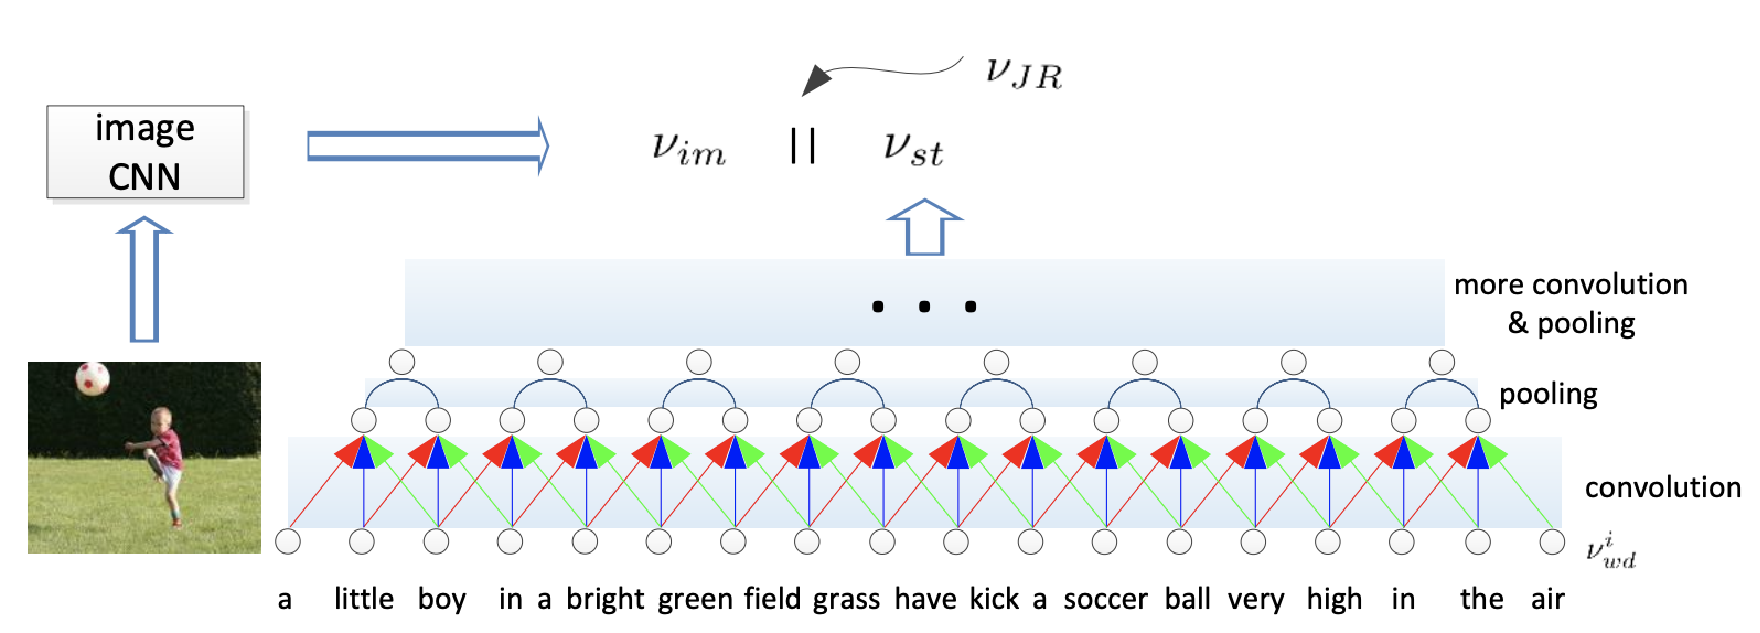
\includegraphics[width=\textwidth]{mcnns3.pdf}
\caption{The sentence-level matching CNN and composed phrases. \cite{ma2015multimodal}}
\label{fig:mccns3}
\end{figure}

Sentence level matching used the last feature for stitching.

From the result, it can be seen that the final ensemble effect is the best, but the performance of the single model is about average.

\subsection{Dual-Path Convolutional Image-Text Embedding}

The problem to be solved in this work \cite{zheng2017dualpath} is also the problem of image and text matching. Unlike the previous two works, it does not use front fusion (generally, the effect of front fusion is better than post fusion). But some interesting ideas were introduced.

\subsubsection{Architecture}
The merit of this network structure is the introduction of residual in text's encoder, which solves the problem of matching images and texts after fusion.

\begin{figure}[h!]
\centering
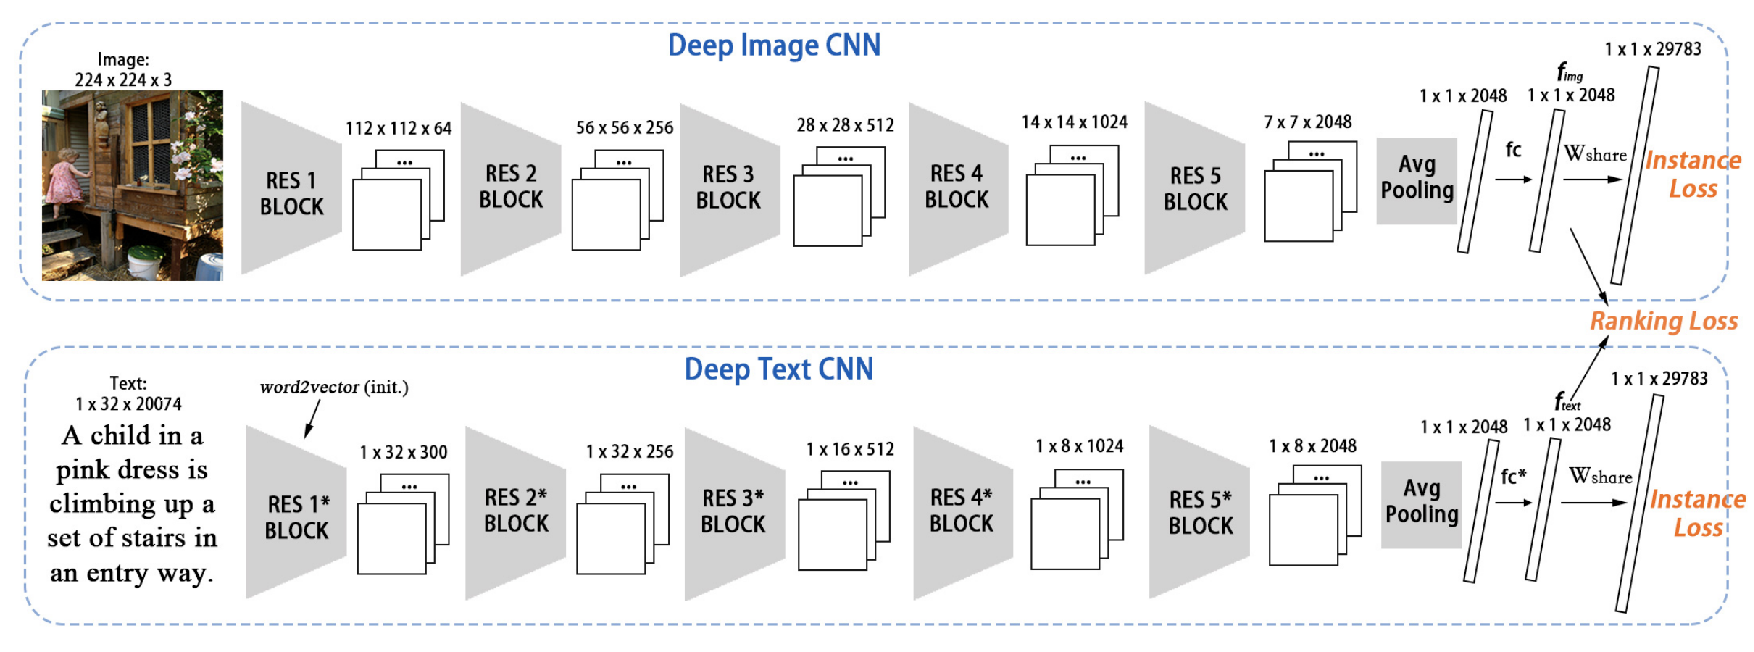
\includegraphics[width=\textwidth]{dpcit1.pdf}
\caption{Architecture of 2 Convolutional Neural Networks \cite{zheng2017dualpath}}
\label{fig:dpcit1}
\end{figure}

\subsubsection{Loss function}
Instance loss was widely discussed in the loss function. The so-called instance loss is the task of doing graphic and text matching. Each pair is used as an instance, and then a \verb|softmax| classifier is used to learn the loss function.

The idea is to adapt the algorithm to the data, that is, to convert the matching problem into a classification problem.

This kind of transformation risk is quite large because our query is diverse; we can never exhaust all query and image pairs, so the basic idea is to achieve it on a multitasking basis.

Before explain multitask loss, we firstly focus on the ranking loss.

The general definition of ranking loss is as follows:

$$
l\left(x_{n}, y_{p o s}, y_{n e g}\right)=\max \left(0, \mu-S\left(x_{n}, y_{p o s}\right)+S\left(x_{n}, y_{n e g}\right)\right)
$$

$S$ is the similarity calculation function, and $\mu$ is the minimum margin in which the similarity needs to be guaranteed. Such ranking loss only considers the loss of $x$ as the matching object, but does not consider $y$. Since $x$ and $y$ are a pair, a two-way loss is required.

Based on this problem, the author proposes the following Ranking loss loss function:

$$
L_{r a n k}=\max \left(0, \alpha-D\left(I_{a}, T_{a}\right)+D\left(I_{a}, T_{n}\right)\right)+\max \left(0, \alpha-D\left(T_{a}, I_{a}\right)+D\left(T_{a}, I_{n}\right)\right)
$$

The front part is Ranking Loss of Image, and the back part is Ranking Loss of Text.

So the final author's loss consists of a total of 3 parts, namely Ranking loss, visual Instance loss, and text Instance loss.

$$
L=\lambda_{1} L_{r a n k}+\lambda_{2} L_{v i s u a l}+\lambda_{3} L_{t e x t u a l}
$$

where $\lambda_{1}, \lambda_{2}, \lambda_{3}$ are predefined weights for different losses.

\subsubsection{Some Interesting Tricks}
This work contains many interesting tricks to achieve better results which we will point out as follows.

\begin{enumerate}
    \item Embedding models initialised with \verb|word2vec| are better than random initialisation.
    \item Sentence jittering, the model randomly adds a certain amount of zero padding to the beginning and end of the sentence.
    \item Instance loss finally shares a same weight parameter to ensure that the information of two different modalities is mapped to the same space.
\end{enumerate}

Two stage training is also the highlight of this article:

\begin{itemize}
    \item Stage-I. At this stage, text residual network is firstly trained. Then it fixes the ranking loss and image in CNN models, so that the CNN of text can be trained. The reason of doing this is the network of text was randomly initialised. To add ranking loss because the image and text are definitely not in the same semantic space at the beginning, we are worried that this loss will be brought into the network of text. Fixing the image CNN because we do not want the gradient of the image and the gradient of the text to interfere with each other.
    
    \item Stage-II, when text's CNN training converges, adding ranking loss and image CNN to the model, and training end-to-end together, the final result is the best.
\end{itemize}

\subsection{DANs}

The main research contribution of DAN \cite{dan} is to introduce attention mechanism into neural network model. The starting point is relatively obvious: the ultimate problem of image and text matching is the matching problem between the entire text and the entire Image, however, this problem is more challenging to solve, so a basic solution is to split the tasks. Text is composed of different words, while image is composed of different regions. If we can match the words of text to the regions of image, this problem will become simpler.

The basic idea is to use the attention mechanism to match text words with image regions in the network automatically. The author cites two types of attention mechanisms: visual attention and text attention.

Both types of attention used the previous state and determine the ``position'' of attention for the next state.

\subsubsection{Visual Attention}
The formula for visual attention is:

$$
\mathbf{h}_{\mathbf{v}, n}^{(k)} =\tanh \left(\mathbf{W}_{\mathbf{v}}^{(k)} \mathbf{v}_{n}\right) \odot \tanh \left(\mathbf{W}_{\mathbf{v}, \mathbf{m}}^{(k)} \mathbf{m}_{\mathbf{v}}^{(k-1)}\right)
$$
$$
\alpha_{\mathbf{v}, n}^{(k)} =\operatorname{softmax}\left(\mathbf{W}_{\mathbf{v}, \mathbf{h}}^{(k)} \mathbf{h}_{\mathbf{v}, n}^{(k)}\right)
$$
$$
\mathbf{v}^{(k)} =\tanh \left(\mathbf{P}^{(k)} \sum_{n=1}^{N} \alpha_{\mathbf{v}, n}^{(k)} \mathbf{v}_{n}\right)
$$


All $\mathbf{W}$ in the formula are parameters that the network needs to learn, $\mathbf{h}$ is the hidden state, and $\mathbf{m}$ is the memory vector.

\subsubsection{Textual Attention}
The formula for textual attention is:

$$
\mathbf{h}_{\mathbf{u}, t}^{(k)} =\tanh \left(\mathbf{W}_{\mathbf{u}}^{(k)} \mathbf{u}_{t}\right) \odot \tanh \left(\mathbf{W}_{\mathbf{u}, \mathbf{m}}^{(k)} \mathbf{m}_{\mathbf{u}}^{(k-1)}\right)
$$
$$
\alpha_{\mathbf{u}, t}^{(k)}=\operatorname{softmax}\left(\mathbf{W}_{\mathbf{u}, \mathbf{h}}^{(k)} \mathbf{h}_{\mathbf{u}, t}^{(k)}\right)
$$
$$
\mathbf{u}^{(k)}=\sum_{t} \alpha_{\mathbf{u}, t}^{(k)} \mathbf{u}_{t}
$$

The step size $\mathbf{K}$ of the two Attentions is a super parameter, and the author proves that $\mathbf{K}=2$ is the best in experiments.

\subsubsection{Visual and Textual Representation}

The visual features use the features of the second layer of Resnet or VGG, and the text features use the features of bidirectional RNN (LSTM). The visual features are shown in the following Figure \ref{dan1}:

\begin{figure}[h!]
\centering
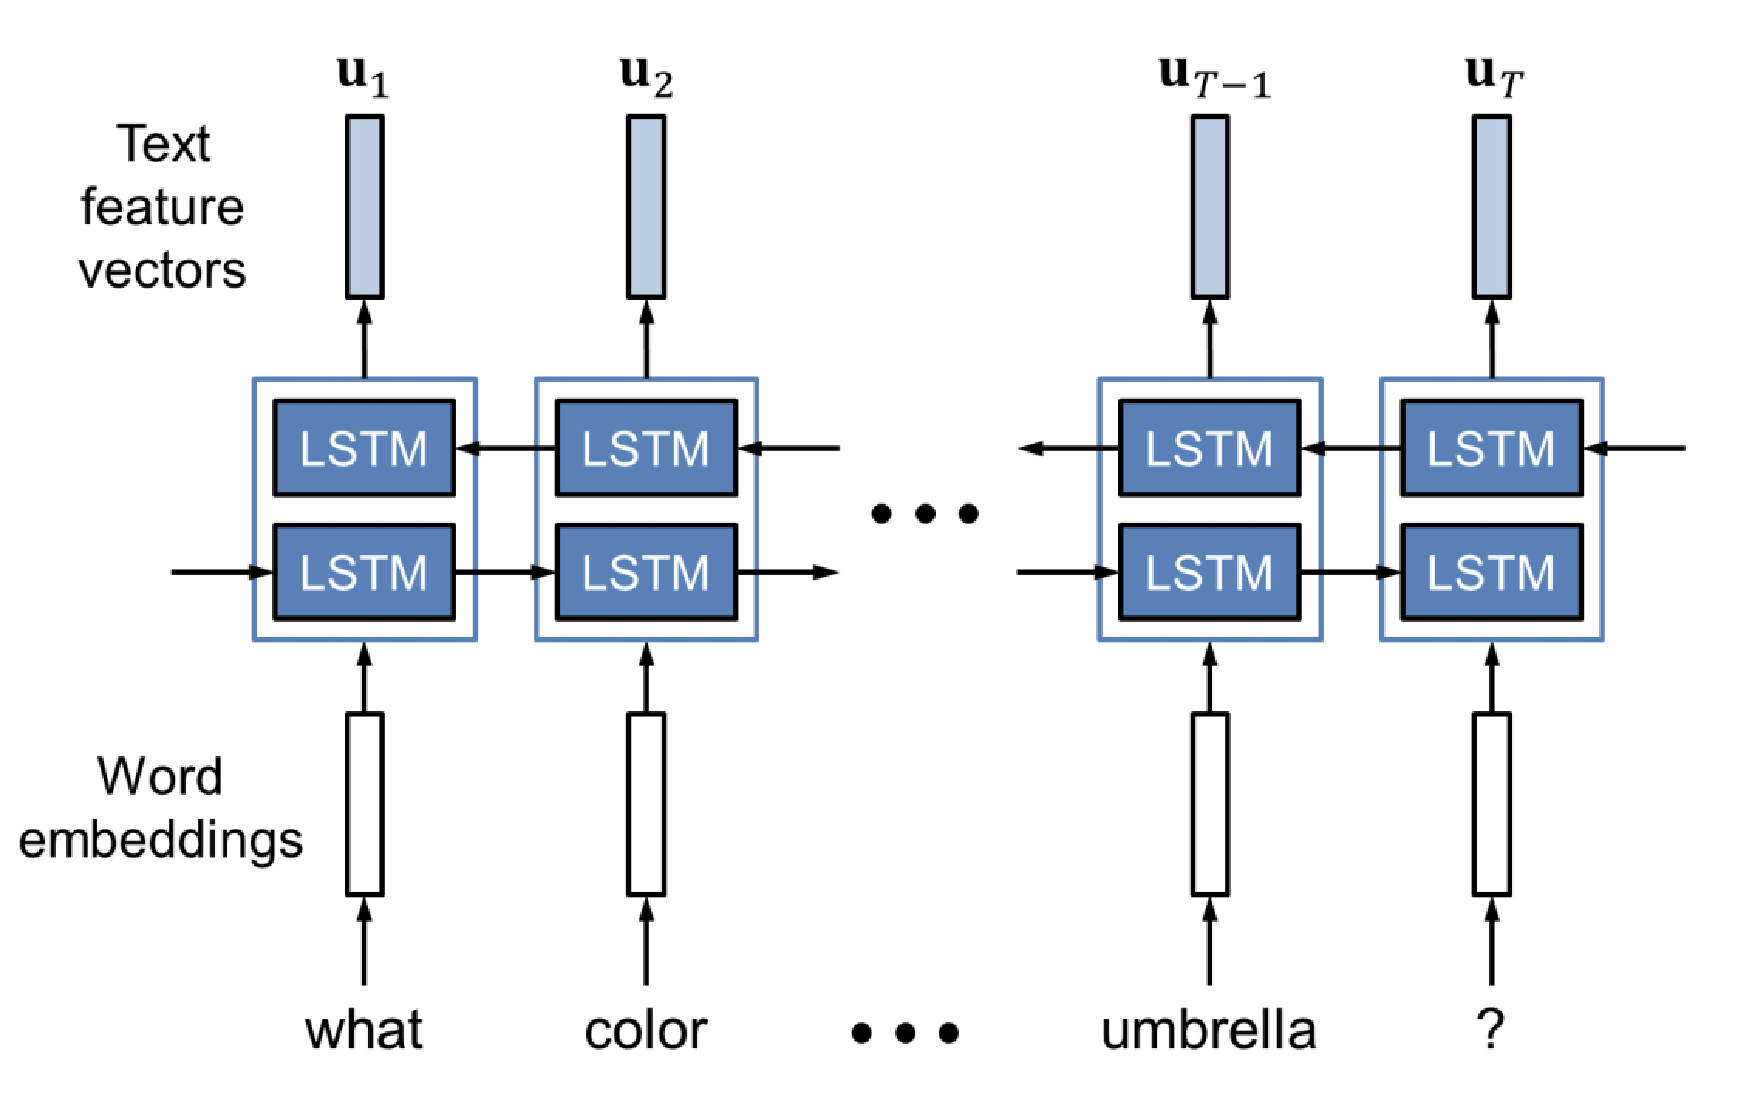
\includegraphics[width=0.8\textwidth]{dans1.pdf}
\caption{Bidirectional LSTMs for text encoding \cite{dan}}
\label{fig:dan1}
\end{figure}

\subsubsection{VQA and Image-Text Matching}

This research solved two different problems which both used the previous attention mechanism. However, the methods of applying attention are different.

\paragraph{Visual Question and Answer}

In the VQA dataset, all the answers are one single word, so in essence, this problem is a classification problem, that is, we need to know which one of the answer sets the question is in the end.

The network structure diagram is displayed as follows in Figure \ref{fig:dan2}:

\begin{figure}[h!]
\centering
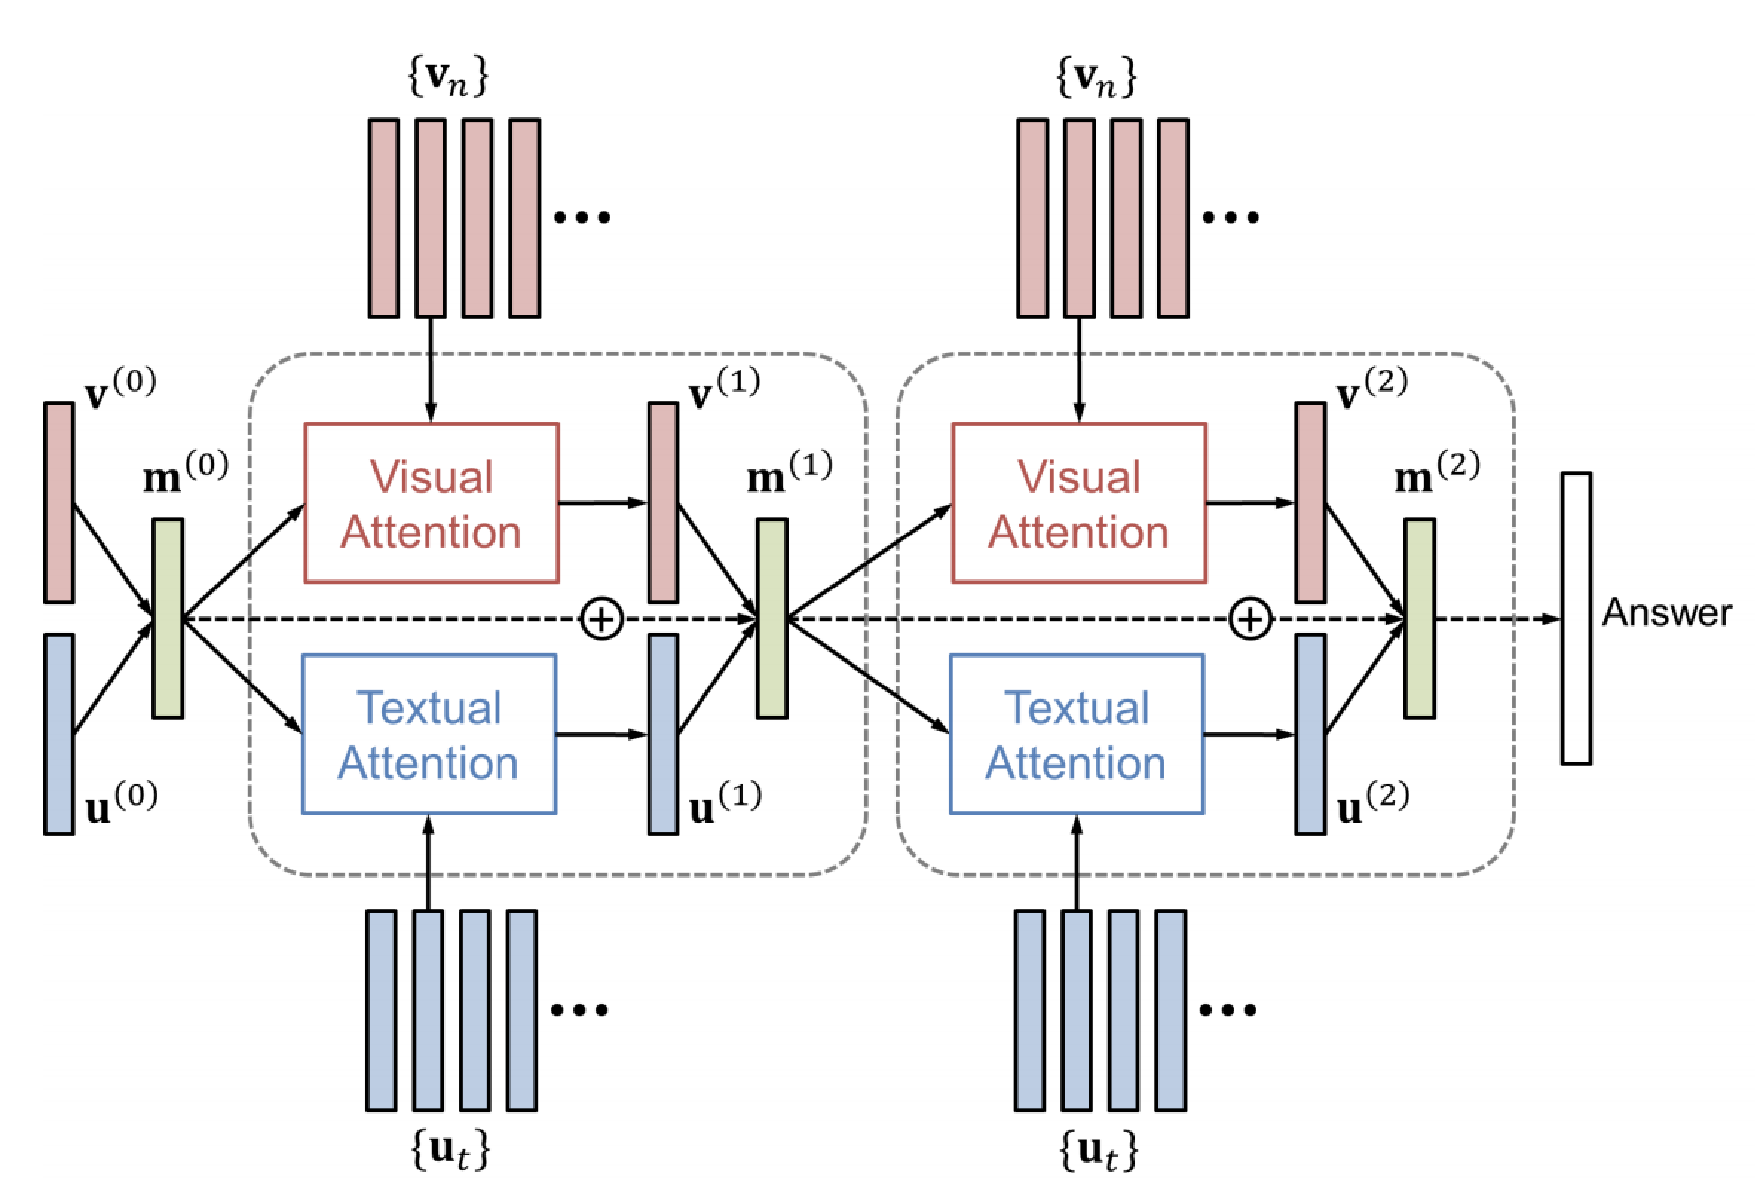
\includegraphics[width=0.8\textwidth]{dan2.pdf}
\caption{r-DAN in case of $\mathbf{K}=2$ \cite{dan}}
\label{fig:dan2}
\end{figure}

As can be seen from the figure, it uses the last memory vector for classification.

The memory vector calculation formula is as follows:

$$
\mathbf{m}^{(k)}=\mathbf{m}^{(k-1)}+\mathbf{v}^{(k)} \odot \mathbf{u}^{(k)}
$$

The initialisation of different parameters is as follows:

$$
\mathbf{m}^{(0)}=\mathbf{v}^{(0)} \odot \mathbf{u}^{(0)}
$$
where
$$
\mathbf{v}^{(0)}=\tanh \left(\mathbf{P}^{(0)} \frac{1}{N} \sum_{n} \mathbf{v}_{n}\right)
$$
$$
\mathbf{u}^{(0)}=\frac{1}{T} \sum_{t} \mathbf{u}_{t}
$$

Because it is an image question answering task, it is necessary to fuse the text features with the image features at each Attention step, and finally output them. According to the last fused features, a \verb|softmax| classifier is sufficient.

\paragraph{Image-Text Matching}
The biggest difference between the image and text matching problem and VQA is solving a ranking problem, so we needs to compare the distance between the two features, so we cannot share the same memory vector.

Corresponding image and text have their own memory vector, their calculation formula is as follows:

$$
\begin{array}{l}
\mathbf{m}_{\mathbf{v}}^{(k)}=\mathbf{m}_{\mathbf{v}}^{(k-1)}+\mathbf{v}^{(k)} \\
\mathbf{m}_{\mathbf{u}}^{(k)}=\mathbf{m}_{\mathbf{u}}^{(k-1)}+\mathbf{u}^{(k)}
\end{array}
$$

The network structure is shown as follows in Figure \ref{dan3}:

\begin{figure}[h!]
\centering
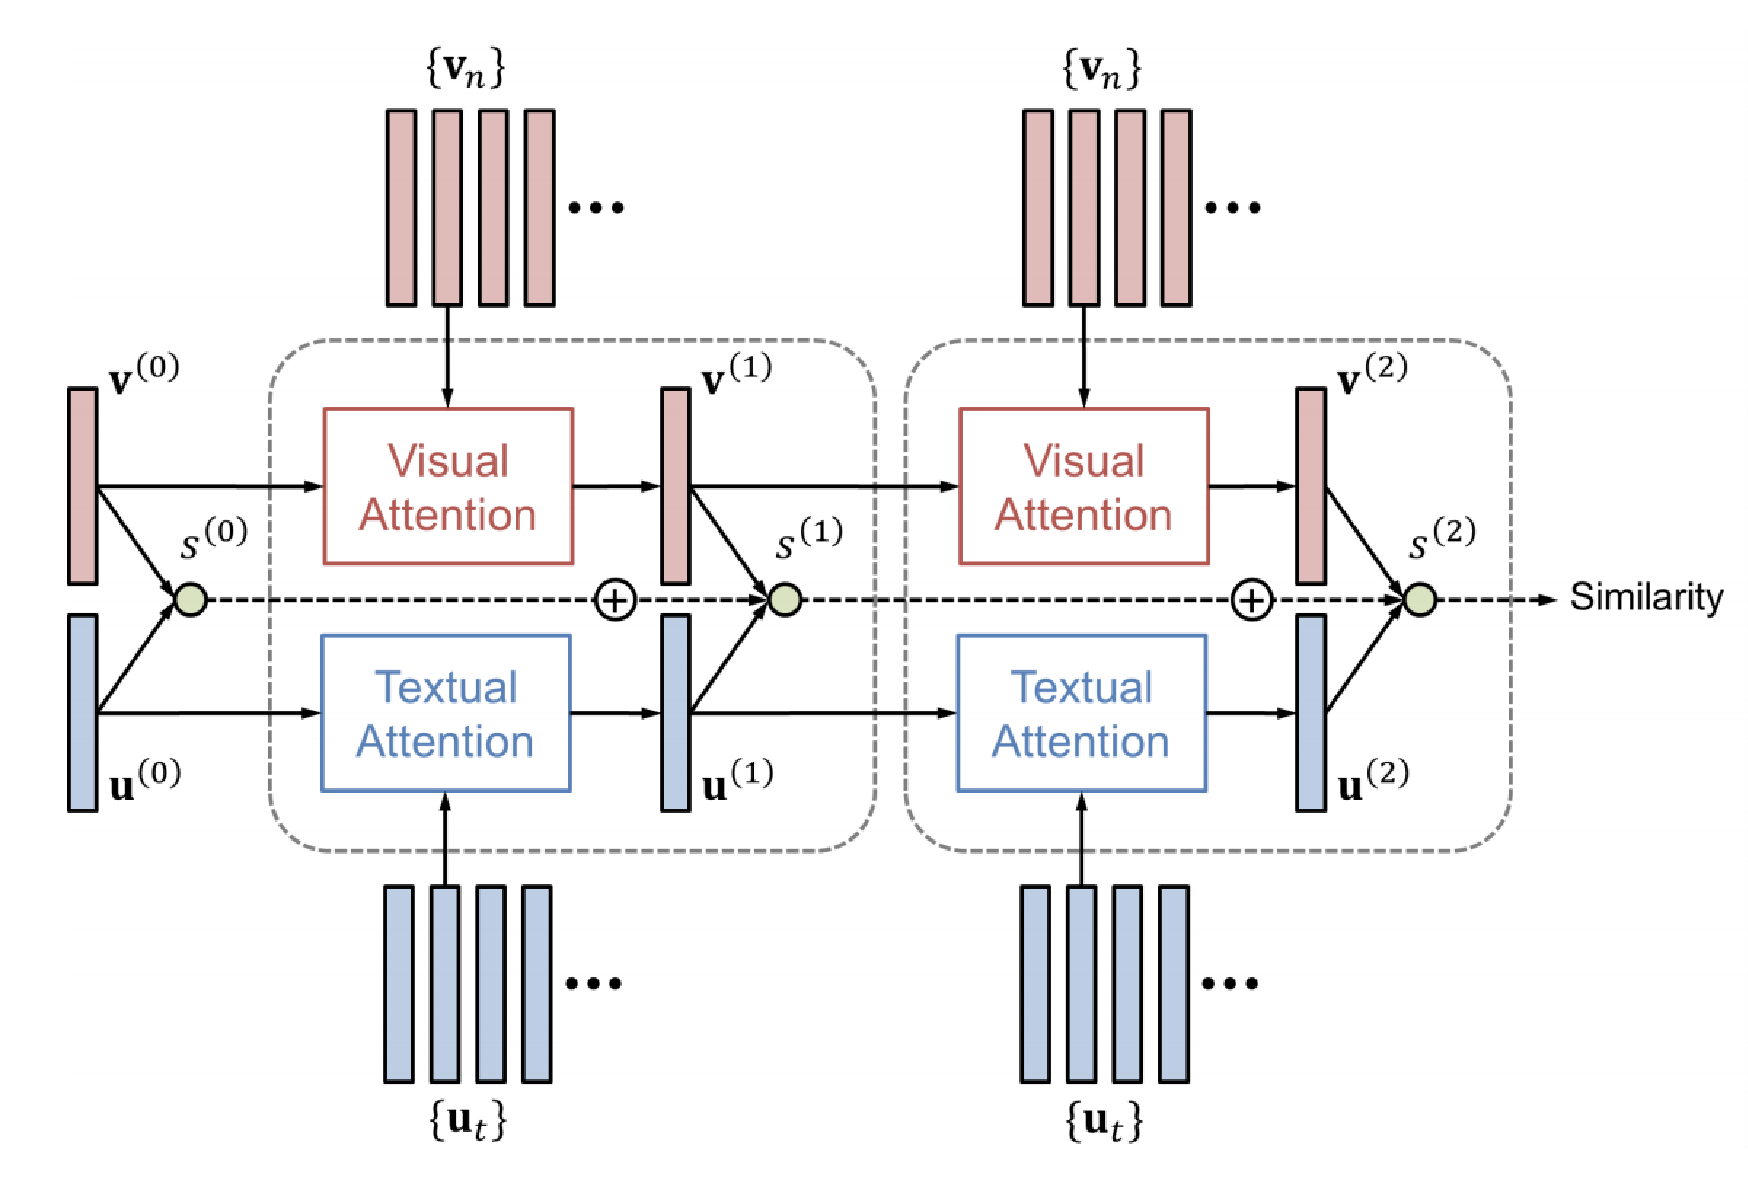
\includegraphics[width=0.8\textwidth]{dan3.pdf}
\caption{m-DAN in case of $\mathbf{K}=2$ \cite{dan}}
\label{fig:dan3}
\end{figure}

In the final experiment, the author used the same Ranking Loss as in the previous work. One difference is that each step of Attention will generate a matching vector. What is done here is to add all $S$.

\subsection{Summary of Image-Text Alignment Related Works}
Throughout these papers, all models are dealing with graphic and text fusion, that is, multi-modal fusion. One of his most basic starting points is that the encoder models for text and images must be good enough, which is the first one, convolution in the article (it seems that Recurrent neural network can also be used).

With an excellent encoder, the next thing to do is the fusion of features. Currently, there are two ways to fuse features, one is pre-fusion, and the other is post-fusion. Pre-fusion inputs image information and text information to a network for further encoder, and finally uses the task-related network; post-fusion is to directly concate the features from the image text encoder and then input to the task-related network. Generally speaking, pre-converged networks are better than post-converged.

Graphic matching is a matching problem of all sentences and all images. It may be relatively tricky to solve this problem directly, so sometimes it is necessary to split these data into components. 

The other is that there are many tricks in the model training. Sometimes or most of the time, it is not because our idea is not good enough, but because we have insufficient experience in training the model, so we tell us that we must be patient in training the model. The road is right, you can keep going, and it will have good results.

\section{Conclusion of Literature}

There are many research focusing on the field of object detection and image-text alignment. We reviewed the research problem and studies their proposed solutions and methodologies. 

In object detection, the major problem is to extract featured object out from images. Convolutional neural network (CNN) \cite{cnn1} was firstly proposed and became the basis of most of the preceding improved models in the field. There are classic deep learning models like VGG \cite{vgg16} and RCNN \cite{rcnn}, followed by more recently improved ones like Fast RCNN \cite{fastrcnn} and Faster RCNN \cite{fasterrcnn}. These deep learning models significantly helped solve the task of object detection and they can achieve promising results.

For image-text alignment, the primary focus is how to map both image and text to the same semantic space. There are CNN models which was able to apply the convolution operation to text such as m-CNN. Recently, models like DAN focus on applying attention mechanism on neural networks to align different image regions to different text tokens, which greatly improved the quality of image-text alignment. 




%%% Local Variables: 
%%% mode: latex
%%% TeX-master: "thesis"
%%% End: 
\chapter{Coarse-grained Cross Modal Retrieval}
\label{cha:scan}
In Chapter \ref{cha:relatedworks}, we discussed several models proposed to solve the image-text alignment task. However, they all have drawbacks in terms of different aspects. In this chapter I will explain the \textbf{S}tacked \textbf{C}ross \textbf{A}ttentio\textbf{n} Model (SCAN) \cite{scan} as our baseline performing coarse-grained cross-modal retrieval. Followed by discussing how it surpasses other models and why we choose to adopt it as our baseline to solve the problem later in the task of fine-grained cross-modal retrieval for artworks.

The structure of this chapter is as follows. Section 3.1 gives an introduction and motivation of SCAN. Section 3.2 explains the structure and methodologies used in SCAN, also how all its components iterates with each other. Section 3.3 briefly discusses the strengths of the adopted model for coarse-grained cross-modal retrieval. Section 3.4 illustrates the preliminary experimental results on our artwork datasets and the achievement of SCAN. Section 3.5 summarises this section.

\section{Motivation}

There are several models proposed recently to solve the problem of cross-modal retrieval, and many have achieved excellent accomplishments. However, Lee, et al. \cite{scan} mentioned some current existing drawbacks of mainstream image-text alignment models, such as:

\begin{itemize}
    \item Attention mechanism is not considered at all, and the entire image and sentence pair are aggregated together, e.g. VSE++ \cite{vse}.
    \item A bit more refined: calculate the similarity between each region-word, take maximum and add them together as the similarity of the entire pair, e.g. Deep-VS \cite{neuraltalk2}.
    \item With attention used, but a predetermined step-process is used to capture limited semantic alignment, and because the entire feature is sent in, it lacks interpretability, e.g. Dual Attention Networks (DANs) \cite{dan}.
\end{itemize}

Stacked Cross Attention (SCAN) is proposed in a paper published on ECCV by Lee, et al. \cite{scan} in 2018. The paper aimed to combine the above aspects (attention mechanism and using pairs), first extracting the features of the image and sentence, then using attention for each region and word, and finally calculating similarity so that attention is used for finer-grained alignment.

Also, the paper used some of the currently available optimisation methods, such as the use of hard-negative, triplet ranking loss, etc.

We will explain the structure of SCAN model in the next sections.

\section{Image Feature Extraction}
Before we perform any cross-modal retrieval and alignment between image and text, we need to have firstly extract features from images. There are many models we have discussed before in Section \ref{cha:relatedworks}, here we used one of the mentioned models called Faster R-CNN. 

Anderson, et al. \cite{bottomup} proposes a top-down and bottom-up attention model method, which is applied to the related issues of visual scene understanding and prominent question answering system. This is based on the bottom-up attention model (usually Faster R-CNN) is used to extract the region of interest in the image. 

Although this work \cite{bottomup} does not mention the Encoder-Decoder framework, which is the most widely used in the current research, the task of the bottom-up attention model is to obtain the image interest area. Extracting image features is similar to feature encoding the image to achieve the encoding stage Task; and the top-down attention model is used to learn to adjust the feature weights, realise the ``timely attention'' of image content, and generate descriptions word by word, equivalent to the decoding stage.


\subsection{Why Adopt Faster R-CNN?}

\begin{figure}[h!]
\centering
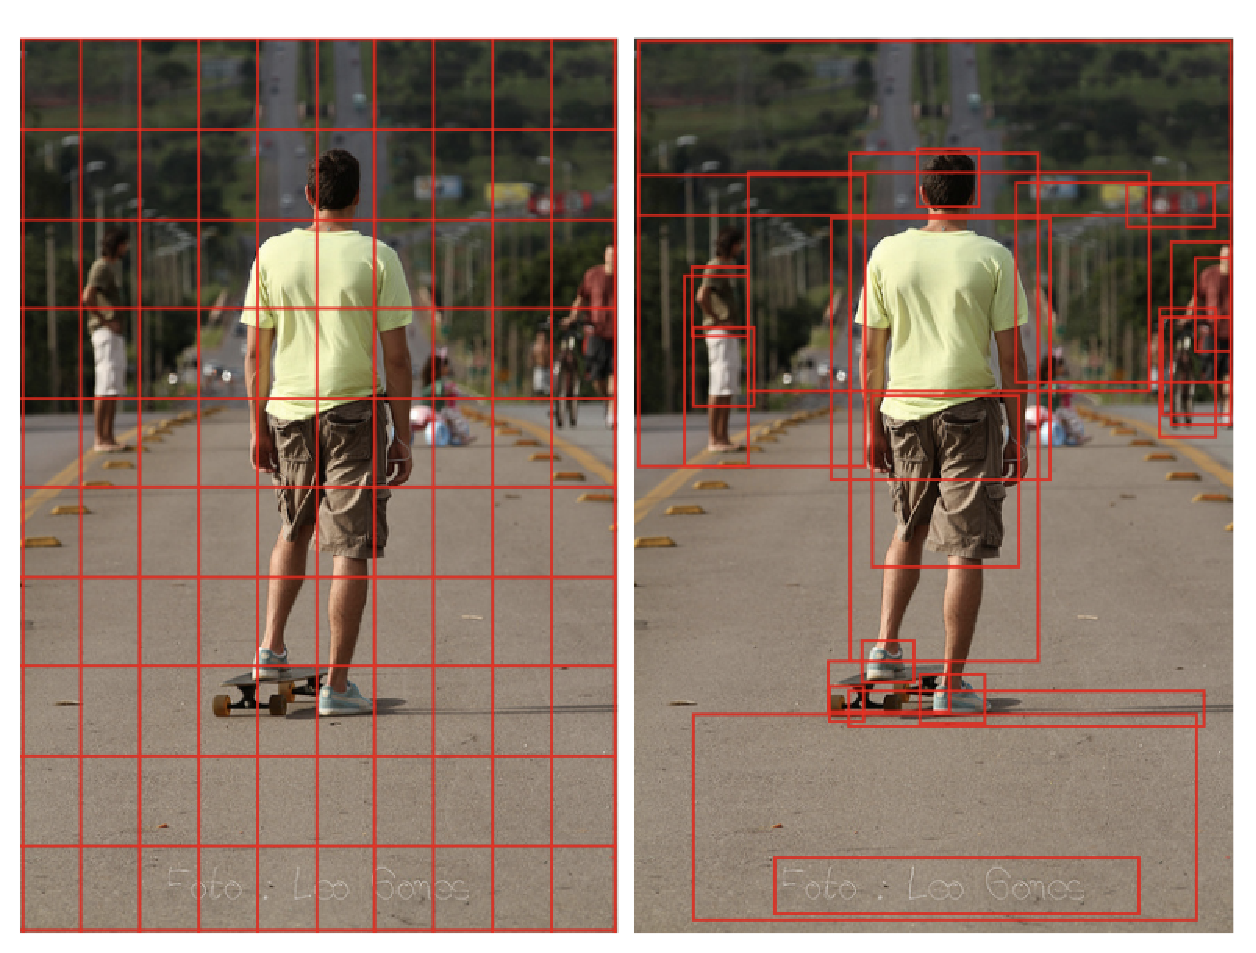
\includegraphics[width=.4\textwidth]{whyfasterrcnn.pdf}
\caption{Faster R-CNN with attention comparing to CNN \cite{bottomup}}
\label{fig:fasterrcnnbottomup}
\end{figure}

It can be seen from the Figure \ref{fig:fasterrcnnbottomup} that using CNN requires more features than R-CNN, and many features are often useless. The target detection method of R-CNN first obtains the interest area for the image, and then applies the target detector to each interest area, so that the image category can be accurately obtained; the CNN method requires the input of the entire image and is used for broad sample classification Of networks are often complex and computationally intensive. In addition, Faster R-CNN improves on previous generations of R-CNN methods and realises the ability to recognise all objects with only one input, which significantly improves processing efficiency.

\subsection{Bottom-Up Attention Model}

From Figure \ref{fig:bottomup} below, it can be seen that the difference from the prior works is that the set of thresholds allows overlapping of interest frames, which can more effectively understand the image content. In this paper, not only the object detector but also the attribute classifier is used for each region of interest, so that a binary description of the object \verb|(attribute, object)| can be obtained. This description is more suitable for practical applications.

\begin{figure}[h!]
\centering
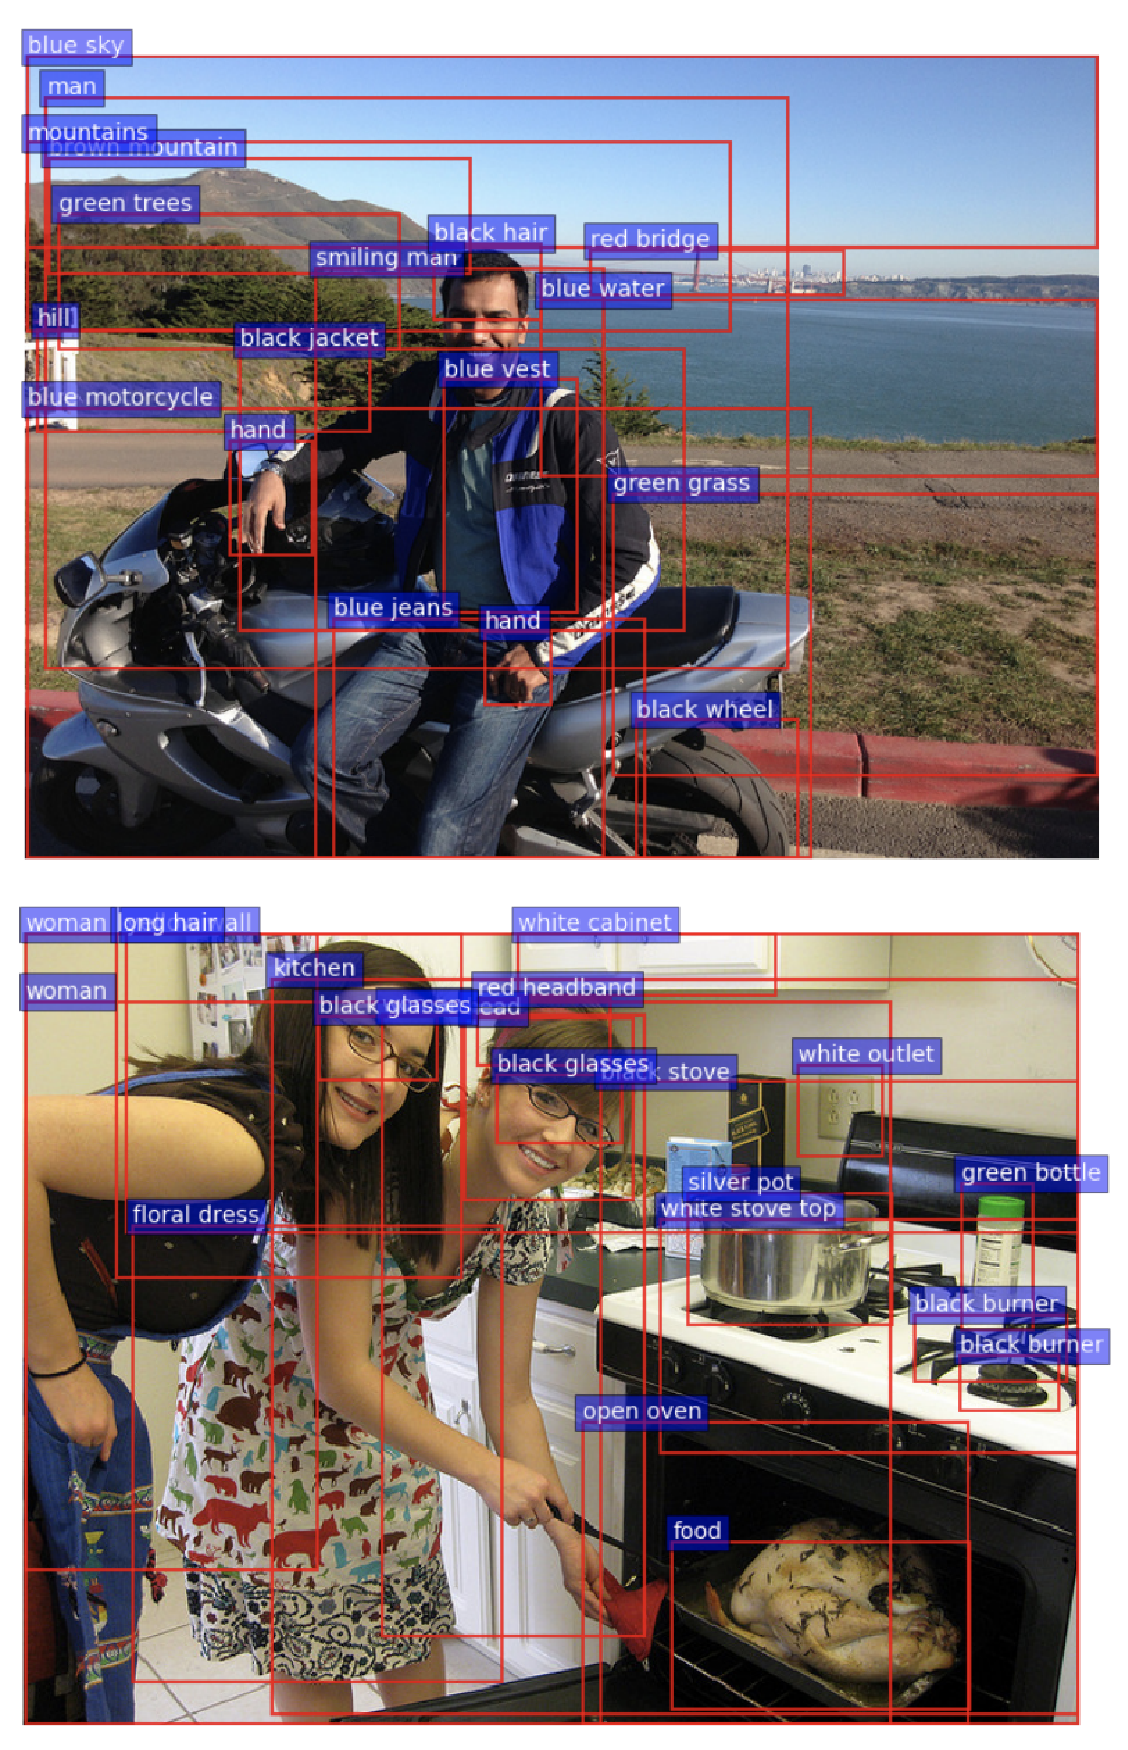
\includegraphics[width=.35\textwidth]{bottomup.pdf}
\caption{What bottom-up attention model captures? \cite{bottomup}}
\label{fig:bottomup}
\end{figure}

\section{SCAN Model}
In this section, we start discussing SCAN with a brief introduction on its structure, followed by in-depth explanations on each specific stages - what is happening behind and why?

\subsection{Brief Structure}
\begin{enumerate}
    \item Use bottom-up attention mechanism \cite{bottomup} to detect the image area and extract the features of the image area;
    \item Map the words in the sentence and their sentence context to feature vectors;
    \item Stacked Cross Attention is used to deduce the similarity of images and text by aligning image regions and word features;
    \item The loss function of SCAN focuses on the hardest negative image-text pairs in each batch (that is, the most unmatched image-text pairs).
\end{enumerate}

Next, we are going to explain each stage in detail.

\subsection{Image-Text Matching}

The process is shown below in Figure \ref{fig:scan1}.

\begin{figure}[h!]
\centering
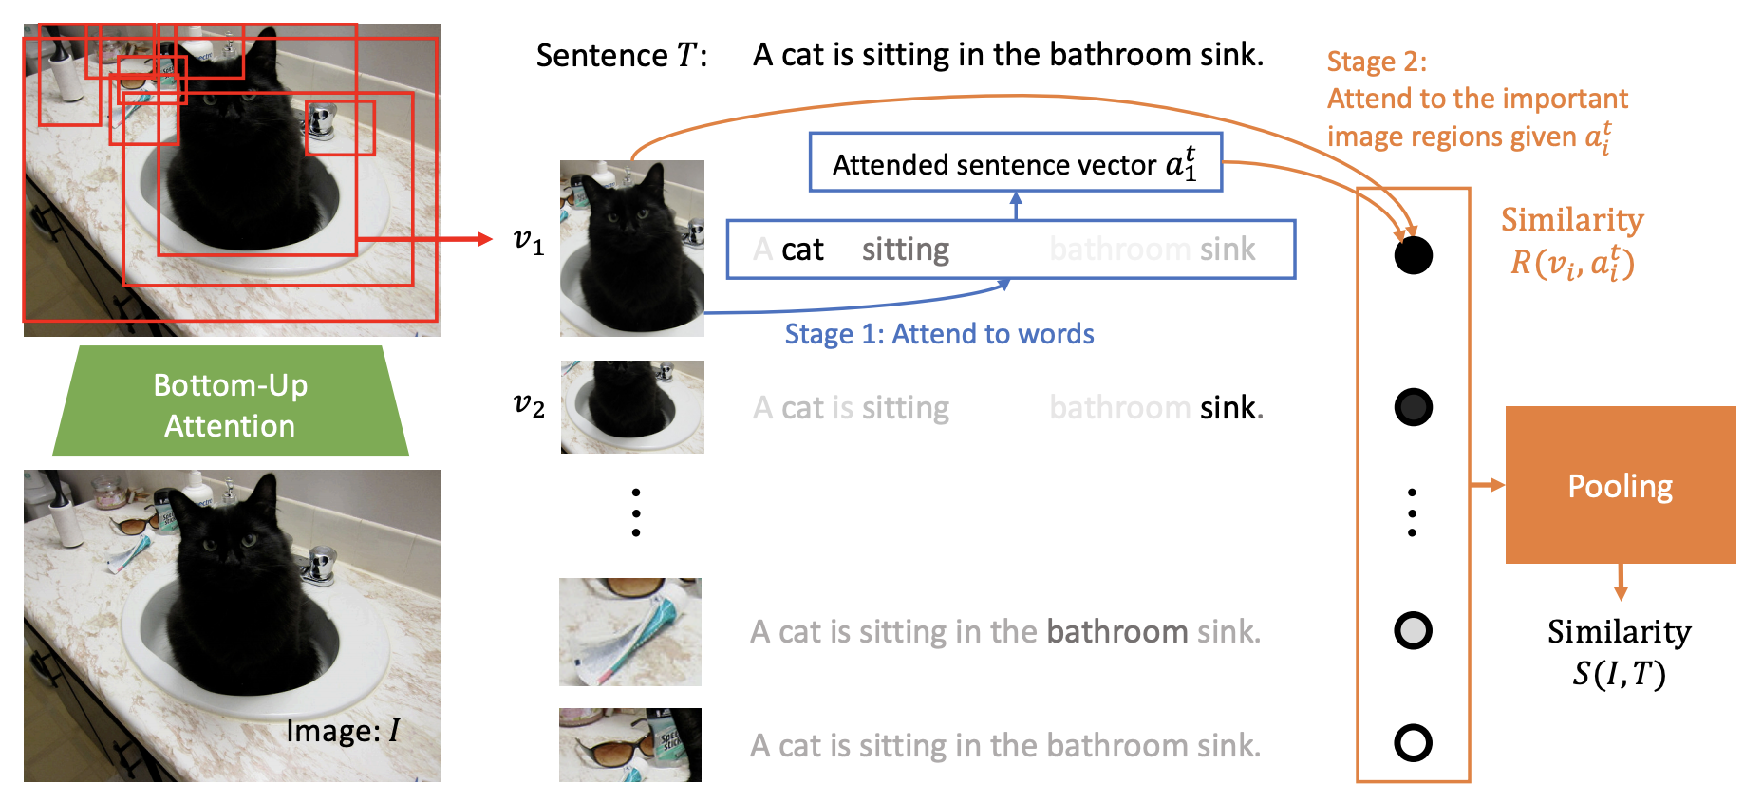
\includegraphics[width=1\textwidth]{scan1.pdf}
\caption{Image-Text Stacked Cross Attention \cite{scan}}
\label{fig:scan1}
\end{figure}

First, use bottom-up attention \cite{bottomup} to extract multiple proposals into features for the image, then map to the same dimensions as the sentence features, and use bi-direction GRU to extract features for the sentence.

Stage 1: calculate the attention representation $a_{i}^{t}$ of all words for each region $i$, and add them together to obtain the sentence representation $a_{i}^{t}$, the formula is as follows:

$$
a_{i}^{t}=\sum_{j=1}^{n} \alpha_{i j} e_{j}
$$

where

$$
\alpha_{i j}=\frac{\exp \left(\lambda_{1} \bar{s}_{i j}\right)}{\sum_{j=1}^{n} \exp \left(\lambda_{1} \bar{s}_{i j}\right)}
$$

Stage 2: calculate the cosine similarity of the $i$-th region and the obtained $a_{i}^{t}$.

$$
R\left(v_{i}, a_{i}^{t}\right)=\frac{v_{i}^{T} a_{i}^{t}}{\left\|v_{i}\right\|\left\|a_{i}^{t}\right\|}
$$

Finally, $i$ areas are superimposed together to get the similarity between image and text, using LogSumExp pooling (LSE), i.e.

$$
S_{L S E}(I, T)=\log \left(\sum_{i=1}^{k} \exp \left(\lambda_{2} R\left(v_{i}, a_{i}^{t}\right)\right)\right)^{\left(1 / \lambda_{2}\right)}
$$

Alternatively, we can
summarise $R\left(v_{i}, a_{i}^{t}\right)$ with average pooling (AVG), i.e.

$$
S_{A V G}(I, T)=\frac{\sum_{i=1}^{k} R\left(v_{i}, a_{i}^{t}\right)}{k}
$$

\subsection{Text-Image Matching}

\begin{figure}[h!]
\centering
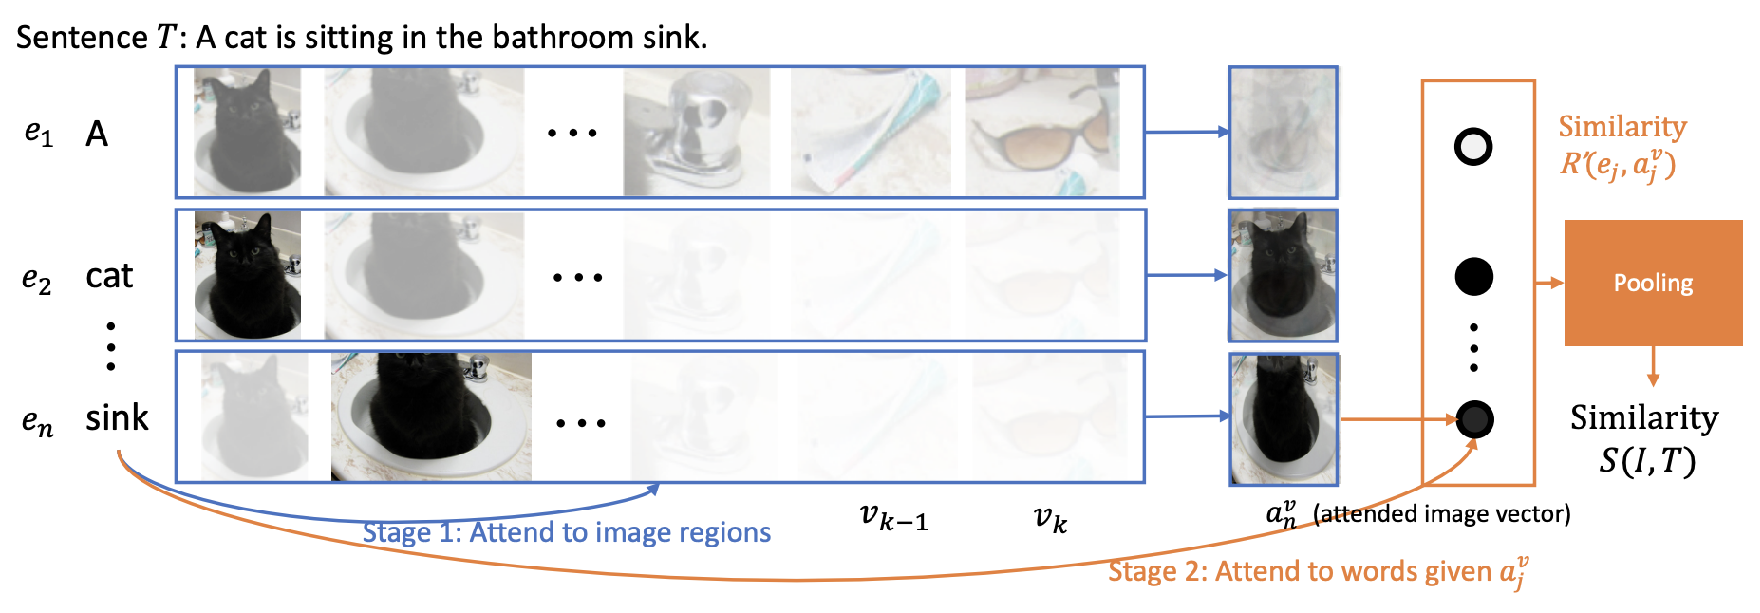
\includegraphics[width=1\textwidth]{scan2.pdf}
\caption{Text-Image Stacked Cross Attention \cite{scan}}
\label{fig:scan2}
\end{figure}

The overall steps correspond exactly to the above, except that each word is used to calculate the similarity with the attention of a picture, which is not repeated here. The process is illustrated in Figure \ref{fig:scan2}.

\subsection{Target Alignment}
Target alignment is essentially the setting of the loss function. In this case, SCAN employs a hinge-based triplet ranking loss with margin $\alpha$.

$$
l(I, T)=\sum_{\hat{T}}[\alpha-S(I, T)+S(I, \hat{T})]_{+}+\sum_{\hat{I}}[\alpha-S(I, T)+S(\hat{I}, T)]_{+}
$$

\begin{itemize}
    \item where $[x]_{+} \equiv \max (x, 0)$ and $S$ is similarity score function (e.g. $S_{L S E}$)
    \item The first sum is taken over all negative sentences $\hat{T}$ given an image $I$; the second sum considers all negative images $\hat{I}$ given a sentence $T$.
    \item If $I$ and $T$ are closer to one another in the joint embedding space than any negatives pairs, by the margin $\alpha$, the hinge loss is zero.
\end{itemize}

For computational efficiency, rather than summing over all the negative samples, it usually considers only the hard negatives in a mini-batch of stochastic gradient descent.

\begin{itemize}
    \item for a pair $(I, T)$, the formula is shown below. e.g. the hard negative of one image is the image that has the highest similarity with the text besides this original pair. (vice versa for text)
    \item Now the hardest negatives are given by $$\hat{I}_{h}=\operatorname{argmax}_{m \neq I} S(m, T)$$ and $$\hat{T}_{h}=\operatorname{argmax}_{d \neq T} S(I, d)$$
    \item The final loss is: 
    $$l_{h a r d}(I, T)=\left[\alpha-S(I, T)+S\left(I, \hat{T}_{h}\right)\right]_{+}+\left[\alpha-S(I, T)+S\left(\hat{I}_{h}, T\right)\right]_{+}$$
\end{itemize}

\subsection{Image and Text Feature Representation}

\subsubsection{Image}Bottom-up attention technique \cite{bottomup}, which is a method of target detection, is obtained based on faster-RCNN. Faster R-CNN first obtains the area of interest for the image, and then applies a target detector to each area of interest, so that the image features can be accurately obtained.

In this paper, the flow for image feature representation is: faster-RCNN, Residual NN (Resnet)101 $\Rightarrow$ 2,048 dimensional features $\Rightarrow$ fully-connected layer transform to $h$-dimensional $\Rightarrow$ get feature set $v$.

\subsubsection{Text}A RNN (recurrent neural networks) is used. In this paper, the flow for text feature representation is: word $\Rightarrow$ one-hot vector showing an index of the word in vocab $\Rightarrow$ embed to 300-dimensional vector $\Rightarrow$ bidirectional GRU map to $h$ dimensions word feature.

\section{Contribution}
Lee, et al. \cite{scan} uses the proposed \textbf{S}tacked \textbf{C}ross \textbf{A}ttentio\textbf{n} (SCAN) to find all potential alignments between the image area and the words, thereby calculating the similarity between the graphics and the text. Existing methods perform fixed-step attention inference so that only a limited semantic alignment can be found at a time, and SCAN can find all possible semantic alignments at the same time. Since the number of semantic alignments varies with different images and sentences, the corresponding relationship inferred by the Stacked Cross Attention method is more comprehensive, thereby making the image-text matching more interpretable.


\section{Preliminary Results}
Here we ran SCAN on two artwork datasets: one ancient Egyptian artworks and one Chinese artworks. For ancient Egyptian artworks dataset, it has 14,353 images in the training set, 1,793 images in the testing/validation set. The other Chinese artworks dataset, there are 6,086 images in the training set, 761 images in the testing/validation set.

For experiment settings, we tested on a Ubuntu machine with Intel Xeon Processor E5-1620 (10M Cache, 3.60 GHz) CPU and a GeForce GTX TITAN X GPU. The specific parameters settings are listed below:

\subsubsection{Settings for image representation}

\begin{itemize}
    \item We used faster R-CNN model and ResNet-101 model pre-trained by \textit{Anderson et al.} on \verb|Visual Genomes| dataset, performs detection of salient regions as bottom-up attention to extract features from images. 
    \item We captured 36 Region of Interests (ROIs) for each image after average pooling and extracted 2,048-dimensional features vector.
    \item We used L2 normalisation (Euclidean distance) into 1,024 joint embedding spaces (same for GRU), these will be used as image feature vectors.
\end{itemize}

\subsubsection{Settings for text representation}

\begin{itemize}
    \item We obtained 300 dimensional word embedding as input to GRU then use embedding matrix to map it into 1,024 joint embedding spaces.
\end{itemize}

\subsubsection{Results}

The following Table \ref{table:resultscan} illustrates the results of running SCAN model on our ancient Egyptian and Chinese art alignment datasets.

\begin{table}[h!]
\centering
\begin{tabular}{lllllll}
                       & \multicolumn{3}{c}{Sentence Retrieval} & \multicolumn{3}{c}{Image Retrieval} \\ \hline
method                 & R@1         & R@5         & R@10       & R@1        & R@5        & R@10      \\ \hline
\multicolumn{1}{r}{}   & \multicolumn{6}{c}{Ancient Egyptian art alignment dataset}                   \\ \hline
SCAN t-i LSE + i-t AVG & 15.3        & 38.5        & 49.9       & 14.1       & 37.6       & 50.2      \\ \hline
\multicolumn{1}{r}{}   & \multicolumn{6}{c}{Ancient Chinese art alignment dataset}                    \\ \hline
SCAN t-i LSE + i-t AVG & 3.3         & 20.4        & 36.1       & 8.0        & 22.9       & 33.8     
\end{tabular}
\caption{Result of SCAN on Artwork Datasets}
\label{table:resultscan}
\end{table}

The results are beyond satisfactory as shown; however, as in this stage, we only used the features obtained using bottom-up attention \cite{bottomup} to train and test, the result may be misleading. As bottom-up attention model was trained on natural images, which means the features we obtained for training and testing set may be irrelevant to those contained in artworks. Noted using entire artwork image and sentence caption to feed SCAN may also lose detailed information in artworks, which will be further discussed in the next chapter.

\section{Conclusion}
Automated image-text mutual annotation would benefit transforming traditional library artwork collection to digital. In this section, we adopted a well-known cross modal retrieval model Stacked Attention as our baseline and evaluated our Egyptian and Chinese artwork datasets on it. Considering the unique representation of artworks, in the next chapter, we will modify SCAN to achieve the cross modal retrieval in a fine-grained level.


%%% Local Variables: 
%%% mode: latex
%%% TeX-master: "thesis"
%%% End: 

% ... and so on until
\chapter{Fine-grained Cross Modal Retrieval}
\label{cha:Method}

In Chapter \ref{cha:scan}, we explained in detail on the structure and principle behind our coarse-grained cross modal retrieval model. As we discussed, there are aspects that we can focus on to
%% SHURONG: change the 'improvements here' as stated in several places in previous chapters. 这个model并不novel, 但是我们把针对artworks的fine-grained retrieval 定位为一个novel task
make improvements, especially on how to focus on the fine-grained features of artworks. In this chapter, we will present our improved model of fine-grained cross modal retrieval.

The structure of this chapter is as follows. Section 4.1 gives a brief introduction on our plans for modifying the previous model into a fragment level. Section 4.2 explains the processed artwork datasets and why the pre-processing is necessary for our model. Section 4.3 proposes our improved fine-grained cross modal retrieval model on fragment level instead of focusing on a whole image or sentence. Section 4.4 shows the results of our presented model running on our annotated artworks datasets. Section 4.5 points out some existing shortcomings of our methodology and potential fields to be focused on in the future. Section 4.6 concludes this section.


\section{Fragment Retrieval}
In this chapter, we are trying to solve the cross modal retrieval task at a fine-grained level, which means we shall not limit our retrieval on the image or sentence level but a fragment level. We applied some changes in the previous model in Chapter \ref{cha:scan}:

\begin{itemize}
    \item Instead of attending between image fragments with each token in sentence captions, here we extract noun phrases from sentence captions to perform mutual attention with image fragments. %% SHURONG:add the purpose of doing this: in order to find fragment-level correspondance between the two modalities.
    \item During the testing process, we replace the original annotations of artworks but adopt manually handcrafted annotations as ground truth, which shall give us a more accurate experiment result.
\end{itemize}

Next, we present our datasets used in this chapter.

\section{Dataset Preparation}
\label{sec:dataprep}
As we mentioned in Chapter \ref{cha:intro}, the same datasets used in this Chapter and Chapter \ref{cha:scan} are from the image caption paper by Sheng et al. \cite{artworkcaption}. For each artwork, two files were available: a high-resolution \verb|jpeg| image file and an accompanying \verb|xml| and \verb|json| file including the metadata.

Python scripts (see Appendix \ref{app:A}) were written to parse the \verb|xml| and \verb|json| files. Instead of using the raw captions, here the textual attributes we use are already processed into phrases. The technique here used is from Handler et al. \cite{nounphrase}, it extracts noun phrases from captions in raw \verb|xml| and \verb|json| files which potentially helped us improve the accuracy as in most cases noun phrases contain more relevant information of artworks.  

As one single artwork can often have more than one annotation existed in its corresponding \verb|xml| file, it is essential to extract all related annotations out and also combine them into one record for training and testing purpose, which saves computational power and simplifies the model input. We generate a combined \verb|.txt| file for each artwork image which contains all related textual attribution then pass it to the noun phrase extraction process in order to achieve the retrieval in a fragment level; results are saved in \verb|json| format. Details are covered in Appendix \ref{app:A}.

Our training tasks are based on these noun phrases and extracted image fragments. The following section demonstrates the architecture of our fine-grained cross modal retrieval model.

\section{Overall Architecture}

The architecture of the fine-grained cross modal retrieval model is depicted in Figure \ref{fig:mainarch}. This model takes full artwork images and full sentence captions as input. The full artwork image input is a (224, 224) sized high-resolution colour picture and the full sentence caption comes from our dataset which contains several descriptions of artworks.

The model has two pipelines processing image and text input from start, for image input, we first detect salient regions as bottom-up attention \cite{bottomup} to extract features from images using faster R-CNN \cite{fasterrcnn} and ResNet-101 \cite{resnet} (mentioned in Section \ref{sec:fasterrcnn}). These obtained image fragments and their representations will be passed into a fully-connected layer, in order to transform them into a joint embedding space with the same dimension of text (i.e. the dimension of GRU explanation in next paragraph).

\begin{figure}[h!]
\centering
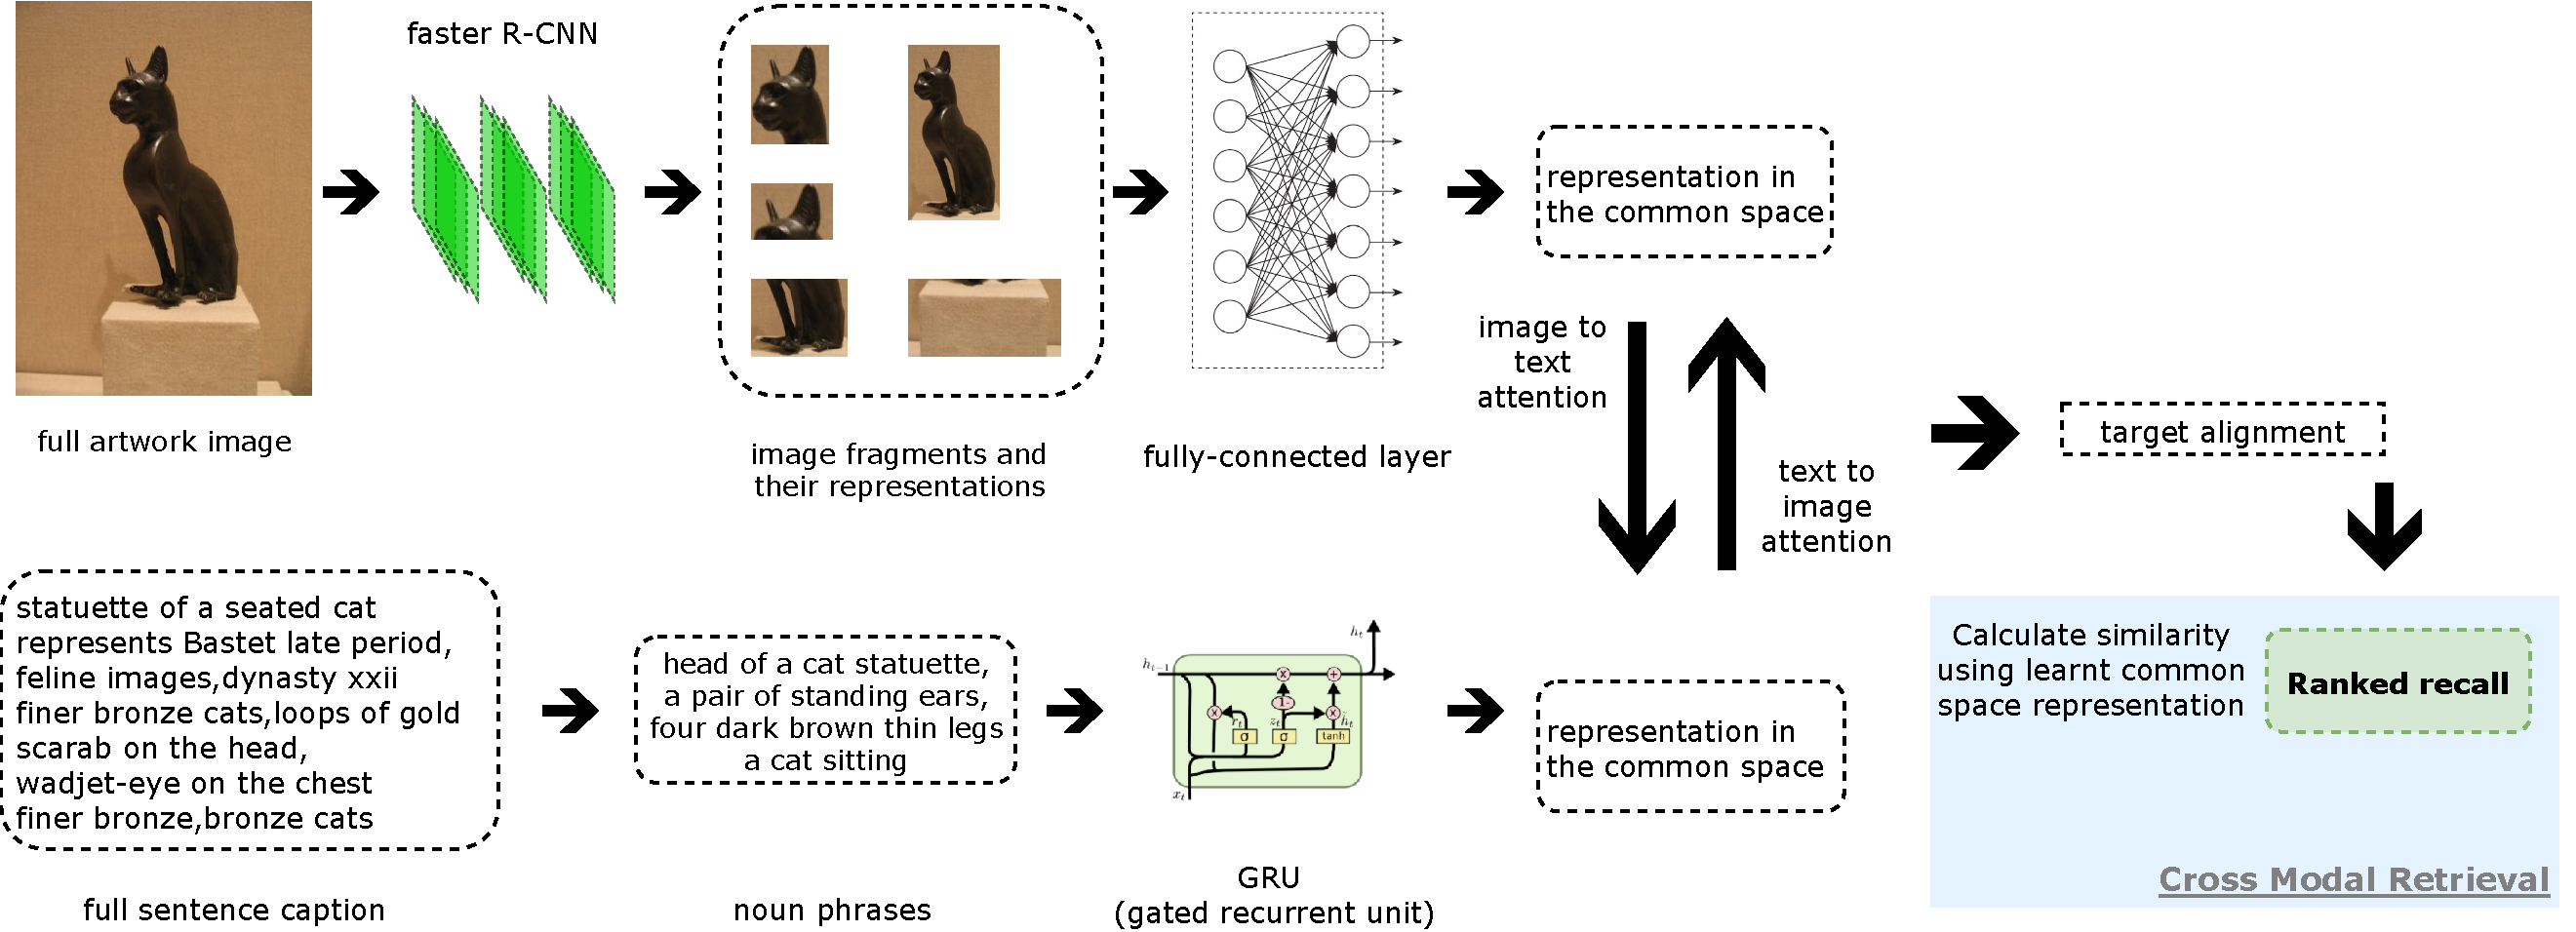
\includegraphics[width=1.0\textwidth]{archinew.pdf}
\caption{Fine-grained Cross Modal Retrieval Model Architecture}
\label{fig:mainarch}
\end{figure}

For full sentence captions as text input, as we mentioned in Section \ref{sec:dataprep}, we do not process the whole sentence directly but first, extract noun phrases out to achieve a finer-grained level. These noun phrases features will be passed into a bidirectional GRU to map them into the same dimension joint embedding space as image features. 

After we learnt image and text representation in a common space, we can use SCAN to attend image to text and attend text to image, in order to get better alignment in between. After computed mutual attention between image and text, we start our follow-up part, which is cross modal retrieval. We use our learnt common space representation to calculate similarity scores between image and text - in this case, cosine similarity; meanwhile, calculate ranked precision and recall for testing.

\section{Experiments}

For experiment settings, we used the same settings and environment as mentioned in Chapter \ref{cha:scan} : Ubuntu machine with Intel Xeon Processor E5-1620 (10M Cache, 3.60 GHz) CPU and a GeForce GTX TITAN X GPU. 

\subsubsection{Settings for image representation}

\begin{itemize}
    \item To save intense labour on retraining model for feature extraction task, we kept the weights pre-trained by Anderson et al. on \verb|Visual Genomes| dataset like in Chapter \ref{cha:scan}for faster R-CNN model and ResNet-101 model and performed detection of salient regions as bottom-up attention to extract features from images. 
    \item We captured 36 Region of Interests (ROIs) for each image after average pooling and extracted 2,048-dimensional features vector.
    \item We used L2 normalisation (Euclidean distance) into 1,024 joint embedding spaces (same for GRU), these will be used as image feature vectors.
\end{itemize}

\subsubsection{Settings for text representation}

\begin{itemize}
    \item We obtained 300-dimensional word embedding as input to GRU then use embedding matrix to map it into 1,024 joint embedding spaces.
\end{itemize}

\subsection{Ground Truth}

For this specific testing task, as we mentioned before, we used our manually annotated ground truth datasets. Each artwork has an updated \verb|xml| file which contains handcrafted image features and textural attributes. Here we show an example of ground truth annotation in Figure \ref{fig:sampledata}.

\begin{figure}[h!]
\centering
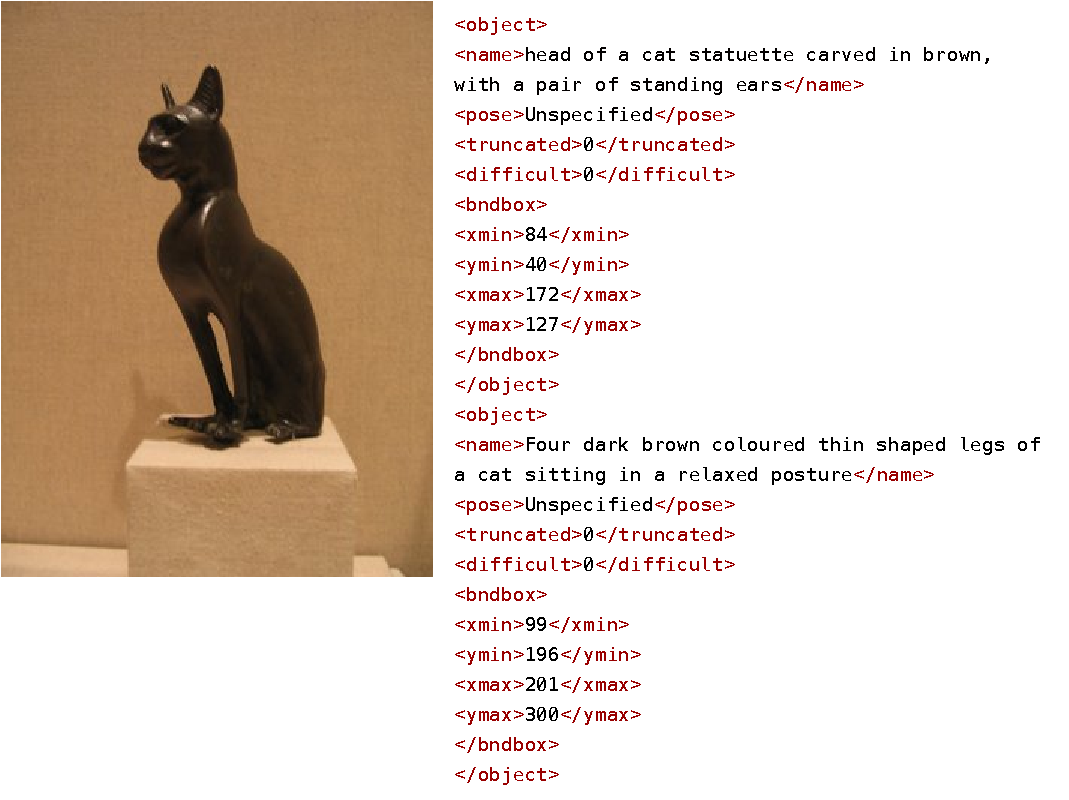
\includegraphics[width=0.8\textwidth]{sampledata.pdf}
\caption{Sample Artwork with Ground Truth Features}
\label{fig:sampledata}
\end{figure}

From Figure \ref{fig:sampledata} we are looking at an Egyptian artwork with a cat sculpture. For all object that exist in the artwork, those are, ``\textit{head of a cat statuette carved in brown, with a pair of standing ears}'' and ``\textit{four dark brown coloured thin shaped legs of a cat sitting in a relaxed posture}'', each of them has a corresponding detailed location, pose, and truncated information attached. 

\subsection{Results}

%%%%%%%%

\begin{table}[h!]
\centering
\begin{tabular}{lcccccc}
\hline
\hline
\multicolumn{1}{c}{} & \multicolumn{3}{c}{Sentence Retrieval} & \multicolumn{3}{c}{Image Retrieval} \\ \hline\hline
\multicolumn{7}{r}{Chinese Artwork Alignment Dataset}                                              \\ \hline
Method               & R@1         & R@5         & R@10       & R@1        & R@5        & R@10      \\ \hline
t-i LSE              & 8.7        & 14.1        & 20.3       & 5.7       & 9.2       & 15.6      \\ \hline
t-i AVG              & 7.9        & 14.4        & 20.6       & 6.2       & 9.6       & 16.2      \\ \hline
i-t LSE              & \textbf{12.8}        & \textbf{20.7}        & 28.7       & \textbf{9.3}       & 15.7       & 22.4      \\ \hline
i-t AVG              & 12.6        & 20.3        & \textbf{28.9}       & 9.1       & \textbf{15.9}       & \textbf{23.2}      \\ \hline
One-directional GRU + i-t AVG  & 15.5        & 18.5        & 24.8       & 7.5       & 14.7       & 19.8      \\ \hline\hline
\multicolumn{7}{r}{Egyptian Artwork Alignment Dataset}                                               \\ \hline
Method               & R@1         & R@5         & R@10       & R@1        & R@5        & R@10      \\ \hline
t-i LSE              & 4.7         & 9.2        & 17.5       & 1.9        & 8.6       & 14.9      \\ \hline
t-i AVG              & 5.1         & 9.4        & 17.9       & 2.2        & 8.9       & 15.2      \\ \hline
i-t LSE              & 5.8         & 11.5        & 20.9       & \textbf{4.7}        & 11.8       & 18.6      \\ \hline
i-t AVG              & \textbf{6.4}         & \textbf{11.6}        & \textbf{21.2}       & 4.4        & \textbf{12.1}       & \textbf{18.7}      \\ \hline
One-directional GRU + i-t AVG  & 5.3         & 10.8        & 20.1       & 3.5        & 10.1       & 16.8      \\ \hline
\end{tabular}
\caption{Result of Fragmented SCAN on Chinese/Egyptian Artwork Dataset}
\label{table:resultfragmented}
\end{table}

Table \ref{table:resultfragmented} present the quantitative results on Chinese and Egyptian artwork datasets where all formulations of our proposed method outperform recent approaches in all measures. Here we denote t-i as Text-Image formulation by text and i-t as Image-Text formulation, AVG as average pooling and LSE as LogSumExp pooling. Like most of the SCAN based models, we tested four different methods by different combinations of formulations and pooling methods. In addition, to check the necessity of bidirectional GRU, we also include a test under one-directional GRU with i-t AVG.

i-t usually surpasses t-i on both pooling methods, and it is evident that using bidirectional GRU improves image annotation R@1 by 2.9 in Chinese artworks and 1.1 in Egyptian artworks, 1.6 and 1.2 for image search. The best result of the model are 13.5 on sentence retrieval (R@1) and 9.9 on image retrieval (R@5) relatively on Chinese artwork dataset; 6.4 on sentence retrieval (R@1) and 4.7 on image retrieval (R@1) relatively on Egyptian artwork dataset. In terms of R@10, our model was able to obtain a 28.6 recall for image annotation task on Chinese dataset which is gratifying and promising considering the strict and detailed ground truth testing set we used.

We noticed that the recalls for sentence and image retrieval on both Chinese and Egyptian artwork datasets are not satisfactorily high. To better understand and evaluate our model, we demonstrate several successful and unsuccessful cross modal retrieval examples in the next section for comparative analysis.

\subsection{Cross Modal Retrieval Examples}
Here we illustrate four typically successful and unsuccessful cross modal retrieval samples of our model: one for each dataset under sentence retrieval and image retrieval. 

\subsubsection{Successful Examples}

\begin{figure}[h!]
\centering
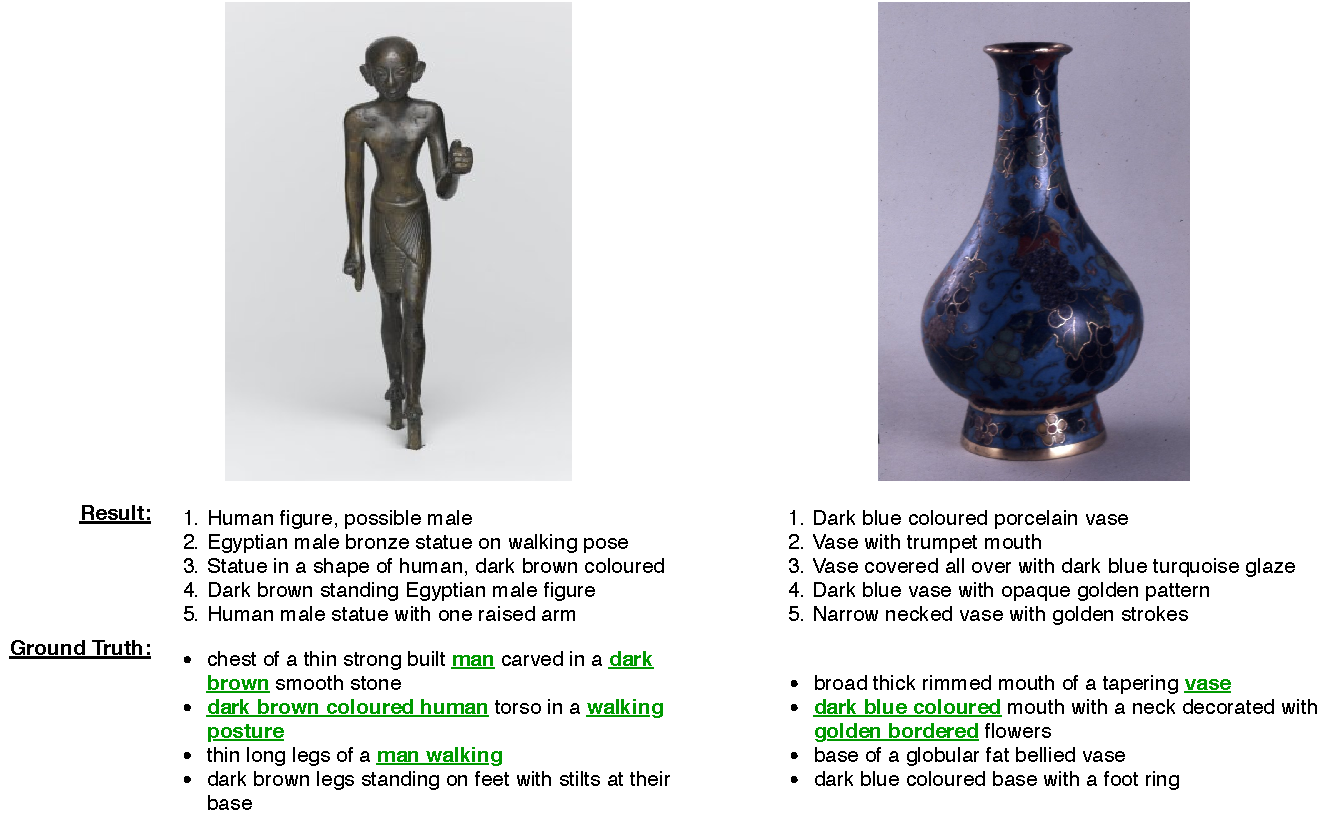
\includegraphics[width=\textwidth]{i2t.pdf}
\caption{Successful Example of Text Phrase Retrieval for Given Image Fragment Queries (fine-grained)}
\label{fig:i2t}
\end{figure}

Figure \ref{fig:i2t} shows two good text retrieval examples from given image queries. The left Egyptian sculpture achieved great noun phrases, the significant features such as standing and walking pose, dark brown colour and the man himself were accurately captured. Although our Egyptian dataset has much more noisy textual attributes, however, after obtained noun-phrase based sentences, we noticed the result was much improved. Comparing to those personification figures in Egyptian artworks, our Chinese artwork dataset has more abstract presentations, and some tiny details can be extremely subtle and hard to distinguish from the background. For instance, this blue vase on the right has a distinctive shape - fat belly, narrow neck and a foot ring. Our model was able to catch a few features such as the colour, category and even the golden patterns. Thanks to the detailed and structured textual descriptions in the training dataset, our model was able to capture most details in the Chinese artworks dataset. However, when it comes to more fine-grained characteristics such as foot ring and flower patterns, in this case, the process becomes more challenging. 

\begin{figure}[h!]
\centering
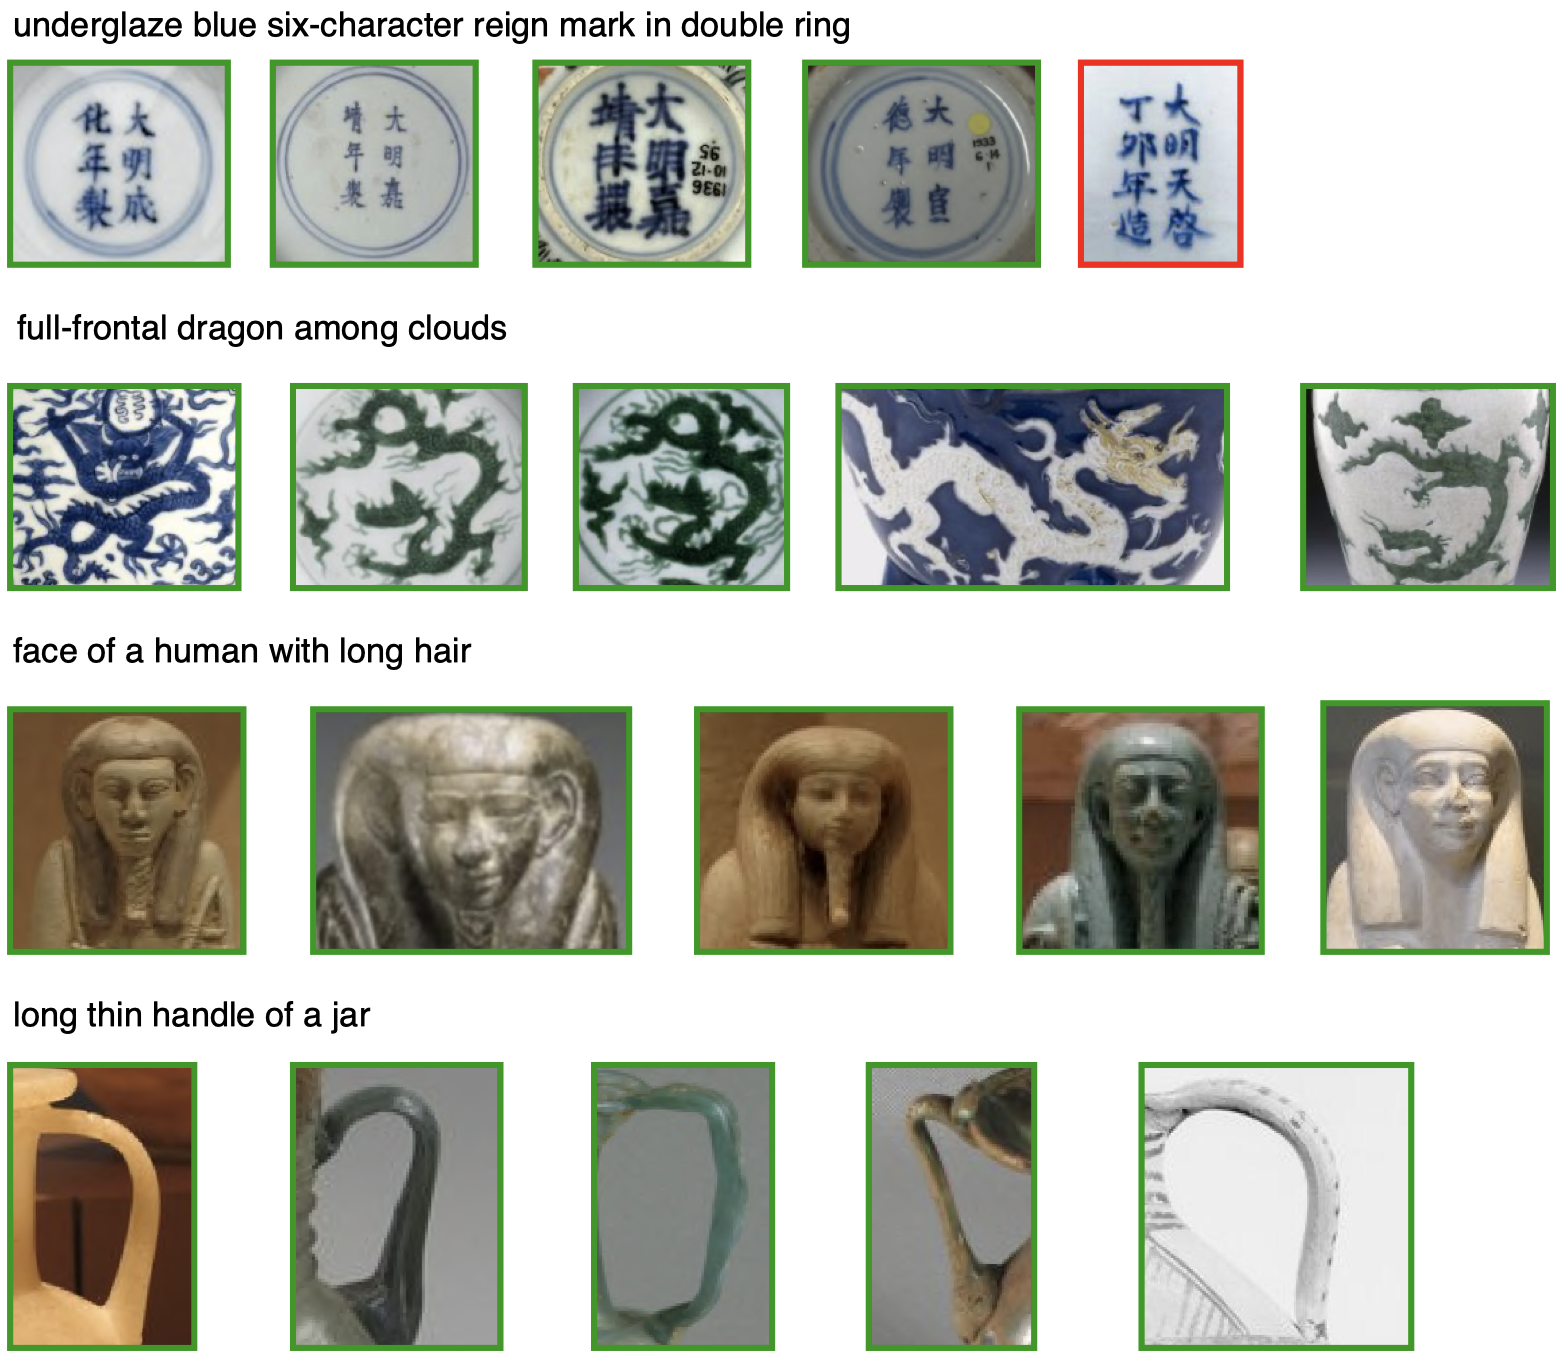
\includegraphics[width=.9\textwidth]{t2i.png}
\caption{Successful Example of Image Fragment Retrieval for Given Text Phrase Queries (fine-grained)}
\label{fig:t2i}
\end{figure}

Next, Figure \ref{fig:t2i} illustrates example image retrieval results from given text queries. The top Chinese art text query is very descriptive and detailed, features like ``bridge'' and ``six cross-patterned circles'' helped our model to distinguish the right image from other similar ones. The bottom Egyptian art text queries are fairly easier than the Chinese one as most of the similar artworks differ in shapes and major gestures such as obvious feature ``broken arms raised to the sky''. However, considering the existing irrelevant noun phrases in the Egyptian artwork dataset such as information on Kingdoms and Pharaoh, it is easier for the model to achieve better results on Chinese artwork dataset than the Egyptian one.


\subsubsection{Unsuccessful Examples}

\begin{figure}[h!]
\centering
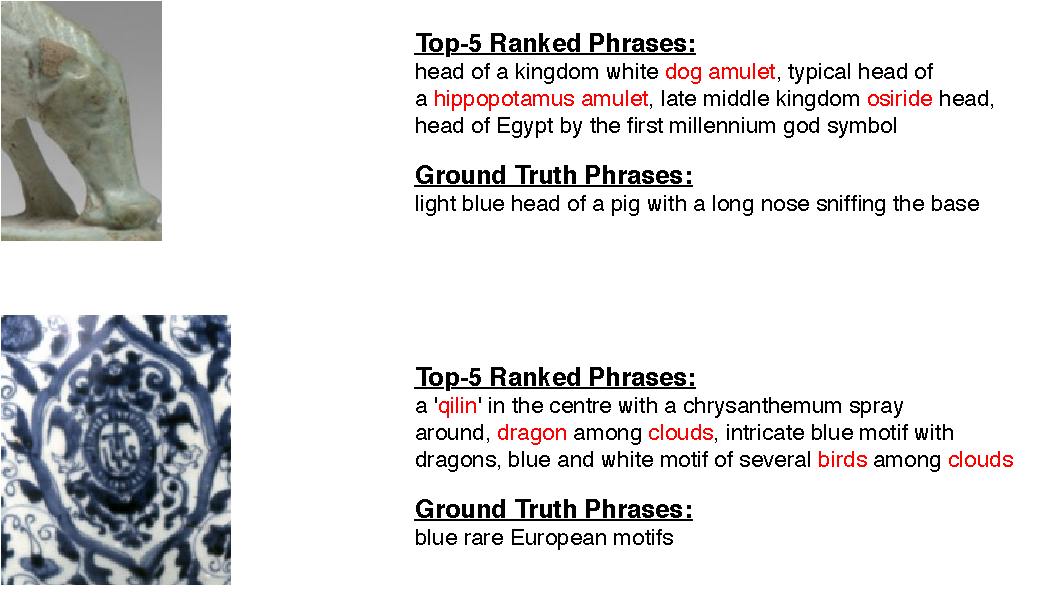
\includegraphics[width=.8\textwidth]{badi2t.pdf}
\caption{Unsuccessful Example of Text Phrase Retrieval for Given Image Fragment Queries (fine-grained)}
\label{fig:badi2t}
\end{figure}

Here Figure \ref{fig:badi2t} displays unsuccessful example text retrieval results from image queries. Our model was not able to identify the left Egyptian pig amulet. It has a tricky shape, and its rare, unique light-blue colour also made it more difficult for the model to retrieve the correct textual descriptions. The similar situation happened in the right Chinese artwork. Our training dataset does not have enough data on jars in this shape, and its complicated patterns increased the degree of difficulty of retrieval task. For instance, its ``kraak'' and ``European motifs'' painting does not appear much in other artworks with the result that our model identified the centre pattern as another more popular one ``qilin''.

\begin{figure}[h!]
\centering
\includegraphics[width=\textwidth]{badt2i.png}
\caption{Unsuccessful of Image Fragment Retrieval for Given Text Phrase Queries (fine-grained)}
\label{fig:badt2i}
\end{figure}

Finally, Figure \ref{fig:badt2i} demonstrates another two unsuccessful example of image retrieval results from text queries. Similar to the text retrieval case we discussed above, the two samples here also have considerably infrequent features. The model usually can pick up the features such as shape and colour, also frequently appeared local characteristics, however, for rare and specific local features such as ``depression'', ``tubular neck'' and ``wide lipped mouth'', the model may get puzzled, which lead to inaccurate and unsatisfactory results.

\subsection{Discussion}
%%
Generally speaking, Chinese artworks surpassed Egyptian artworks on cross modal retrieval tasks - extra detailed descriptive textual attributes provided for fine-grained and varied features in Chinese artworks. There are still a large amount of irrelevant noisy textual attributes in Egyptian artwork dataset even after noun phrase extraction, which significantly complicates the process of distinguishing features. Furthermore, adequate but not excellent recalls are expected. There are three possible causes:

\begin{itemize}
    \item Our training dataset cannot guarantee a balance of features. For example, there are only 6,000 training images for Chinese artworks, and many of them contain diverse shapes and details. Insufficient training features may influence the ability of model, therefore, cause inaccurate retrieval results.
    \item As we adopted new ground truth annotations acting testing purpose, considering these features are mostly handcrafted and being almost 100\% accurate, potentially increased the chance of wrong retrieval results which were retrieved based on original raw training phrases obtained from museum. If we were able to also manually annotate artworks in the training dataset to retrain the model, we suppose the retrieval result shall improve.
    \item One of the crucial requirements for image-text alignment is accurate and proper feature extraction. However, in our case, we used the bottom-up attention mechanism \cite{bottomup}, which was designed and trained on real-world images (\verb|VisualGenome|). We all know that artworks usually have widely different representations and requires unique and specific treatment on feature extraction.
\end{itemize}

Nevertheless, we did not have more time to redesign our feature learning algorithm to make it more adaptable to artwork representations. To improve our model for better fine-grained cross modal retrieval results, in the next section, we dig into some recent research on the aspect of image-text alignment. 

\section{Future Directions}
In this section, we point out some cutting-edge researches on the field of image-text alignment that are related to our methodology as future directions for further improvements. We are going to discuss in two main directions: the way to align image and text and the way to extract image features (representations).

\subsection{Similarity or Fusion?}
Here we investigated recent research in the field of VQA, the problems of VQA and image-text matching have a lot in common. For example, both accept image and text features as input and then encode. If image-text alignment task is treated as a binary classification problem, the only difference is that the output of VQA task is of multiple classes.

Generally speaking, the processing of image-text matching problems can be divided into ``similarity'' and ``classification''. ``Similarity'' is to use the traditional methods such as cosine similarity or dot product to calculate the similarity between image and text in the same embedding space to judge whether it matches or not. The representative methods are SCAN \cite{scan} and VSRN \cite{VSRN}. The ``classification'' method is to use the neural network to fit a function that is better than the cosine similarity, to determine whether the input image and text feature are a match or not. This input comes from two modes and the output The neural network design for a particular result is generally called ``fusion'', which is more common in VQA, and the representative method is MTFN \cite{MTFN}.

Now let us discuss the pros and cons of traditional similarity calculation and fusion by starting from analysing this problem from a theoretical perspective.

First, we look at a general bilinear fusion method proposed in MUTAN \cite{benyounes2017mutan}:

$$
\text {score}=\sigma\left(\left(x_{\text {img}} \odot x_{\text {txt}}\right) \mathbf{W}\right), x \in \mathcal{R}^{1 \times d}, \mathbf{W} \in \mathcal{R}^{d \times 1}
$$

\begin{figure}[h!]
\centering
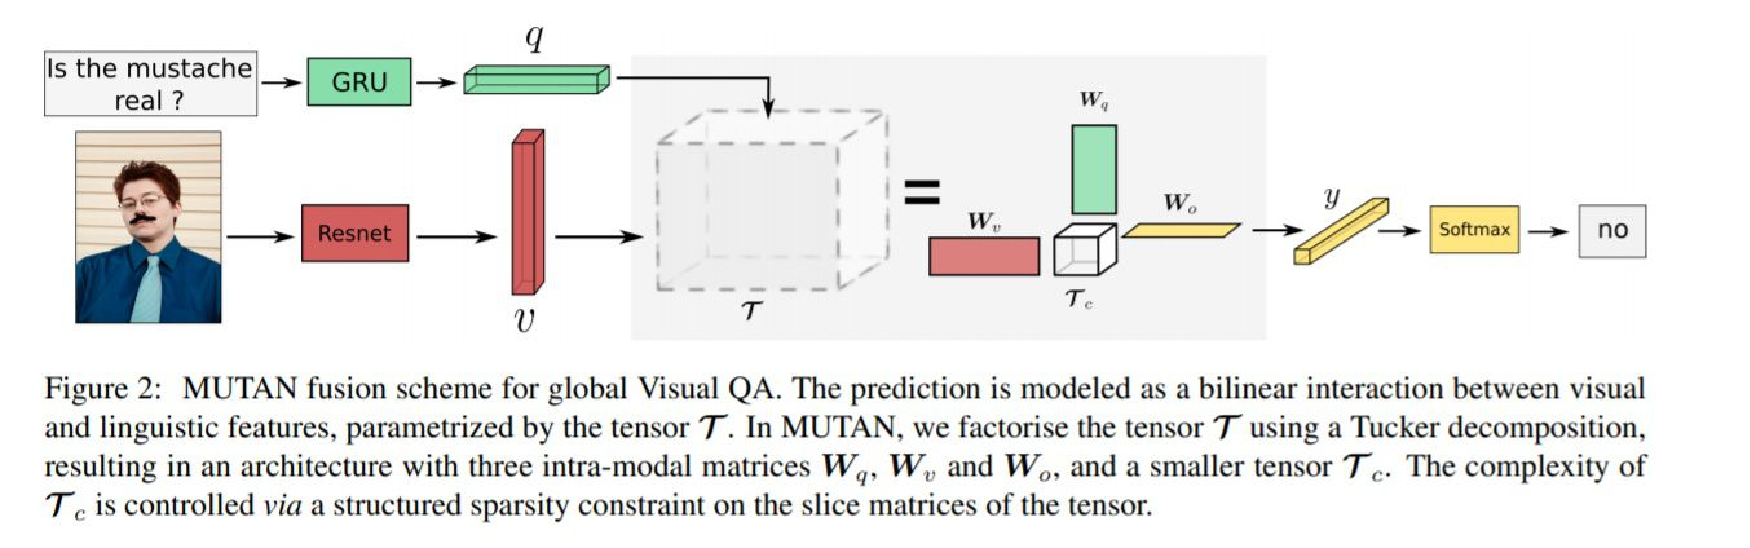
\includegraphics[width=\textwidth]{MUTAN.pdf}
\caption{Bilinear Fusion in MUTAN \cite{benyounes2017mutan}}
\label{fig:mutan}
\end{figure}

Where $x$ represents extracted feature and $\mathbf{W}$ is a learn-able matrix. It is merely to reduce the dimensions after taking the product of the two features and then output the matching probability through the \verb|sigmoid| function. This is also the primary method used in MTFN \cite{MTFN}, which is referred to as bilinear fusion in the following.

Here we use the simplest and most traditional similarity calculation method: dot product here to compare with bilinear fusion:

$$
\text {score}=\sigma\left(x_{\text {img}} x_{t x t}^{\mathrm{T}}\right)
$$

Observing the above two formulas, we can find that bilinear fusion is not much different from the dot product. The dot product is to multiply the corresponding position elements of the two vectors and sum all the elements, while the bilinear fusion is first getting dot product of the corresponding position elements, then get the product of $\mathbf{W}$. This is equivalent to the weighted sum of the elements, that is, when $\mathbf{W}$ is an all-one matrix, bilinear fusion degenerates into a dot product.

From this point of view, bilinear fusion can be understood as weighting different positions when doing dot product when $\mathbf{W}$ is a weight matrix. Weighting helps, but there are two problems:

\begin{itemize}
    \item Optimisation. Can we guarantee a $\mathbf{W}$ better than the all-one matrix?
    \item Design issues. The dimension of the weight matrix is $d\times1$, that is, in the inference, for the element product of any pair of graphic features, the weight of each element position is identical, which is unreasonable.
\end{itemize}

In many experiments, it has not been shown that fusion must perform better than dot product, and dot product is obviously more straightforward and faster than fusion.

\subsubsection{Early Fusion}
There are many improvements to fusion this year, one of the most widely discussed is early fusion. ``Early'' means that comparing to the bilinear fusion mentioned above, it put the multi-modal features into the neural network earlier while there is only one linear layer in bilinear fusion which locates at the end of the entire model. B2T2 \cite{B2T2} compared early fusion and late fusion on the Visual Commonsense Reasoning (VCR) dataset \cite{zellers2019vcr}, and concluded that early fusion usually works better. However, it can be seen from Figure \ref{fig:fusionb2t2} shown below that this comparison can be somewhat unfair, but at least early fusion added more detection information.

\begin{figure}[h!]
\centering
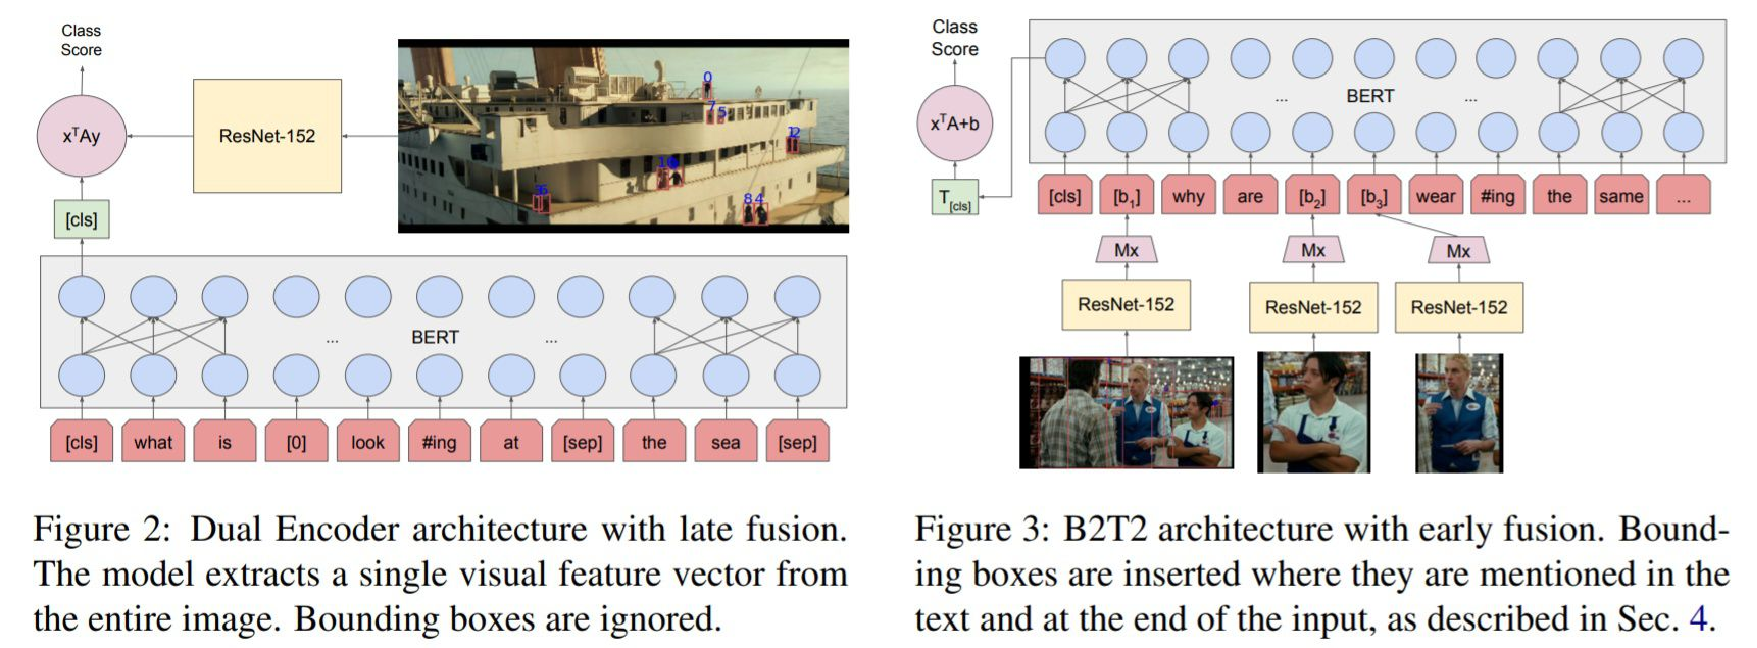
\includegraphics[width=\textwidth]{fusion.pdf}
\caption{Late Fusion (left) \& Early Fusion (right) in B2T2 \cite{B2T2}}
\label{fig:fusionb2t2}
\end{figure}

It should be noted that early fusion is mentioned in many papers, but the structural designs were slightly different, such as RAMEN \cite{ramen}.

Obviously, early fusion has contributed a lot to this aspect, and its performance on VQA is also relatively comparable, but we have not seen enough reliable evidence that early fusion completely exceeds late fusion represented by bilinear fusion. However, at least some aspects have shaken the dominance of bilinear, and these early fusion methods are slightly coarse and have the potential to be better designed. We can expect some future works to break this paradigm.

Back to image-text matching, if the idea of RAMEN \cite{ramen} early fusion is introduced into the research, considerable progress may be made.

\subsection{Better Representation Learning?}

It seems that the most critical factor affecting the alignment task is the characteristics/feature learnt by the network, and the calculation of similarity is not as crucial to a certain extent. VSRN \cite{VSRN} also proved this point by introducing many components to learn features, and then used the most straightforward dot product to achieve the current State-Of-The-Art performance.

Representation learning embodies its importance in earlier work. The bottom-up and top-down \cite{bottomup} attention mechanism used by our previous model has indirectly accomplished many image-text alignment pieces of research. Afterwards, VQA, image-text matching, and image caption all started to use \cite{bottomup} to extract features, which improved SCAN \cite{scan} by a significant amount and shows that a better representation learning model is crucial.

2019 has been a year of the rapid development of representation learning. The leader-board of VCR \cite{zellers2019vcr} has many popular large-scale pre-trained models such as ViBERT \cite{lu2019vilbert}, VideoBERT \cite{sun2019videobert}, UNITE \cite{chen2019uniter} and MoCo \cite{he2019momentum}. Considering the special category of image data we focus on - artworks, here we put more attention on those specialised in artwork feature extraction. Recently, some works \cite{TranslatingArtworks,parttowhole,Art2Real,tan2017artgan,shen2019discovering} have proposed new methodologies for artwork feature extraction and contributed a lot in the field. 


\begin{figure}[h!]
\centering
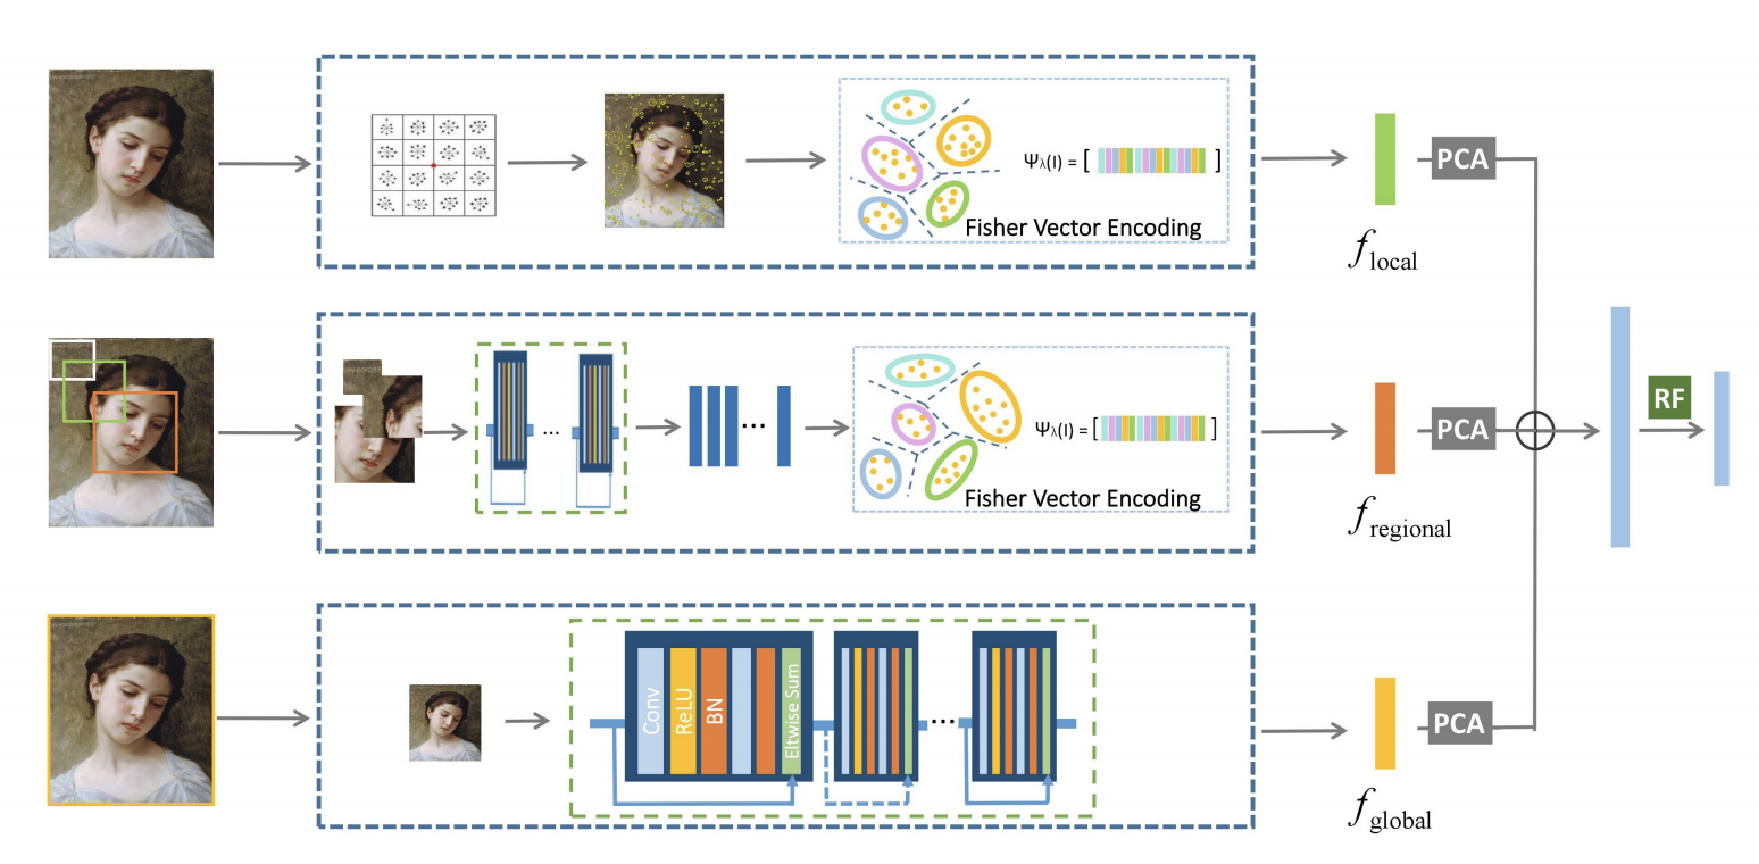
\includegraphics[width=\textwidth]{MTMRoverview.pdf}
\caption{Overview of MTMR Representation Framework \cite{parttowhole}}
\label{fig:mtmroverview}
\end{figure}


Ma el al. \cite{parttowhole} introduced a new methodology for artwork representation in 2017: MTMR (multitask and multi-range). MTMR extracts from the fisher vector based on scale-invariant feature transformation (SIFT) from the painting:

\begin{itemize}
    \item Local, regional and global features
    \item Multiclass area coding structure
    \item Multitask learning framework
\end{itemize}

Figure \ref{fig:mtmroverview} illustrates the overall architecture of the MTMR representation framework. The above, middle and bottom represent different levels of feature extraction using SIFT-based fisher vector: local, regional and global, respectively. Inside each level, there are multiclass area coding and multitask learning structures. These obtained features in different levels will be finally passed to the random forest model as an ensemble mechanism to retrieve a final result.

Figure \ref{fig:mtmrmulti} shows the detailed structure of how multitask learning works in the MTMR framework. The right grey box contains several different tasks which are split to process in parallel. There is a residual network inside the green box, which consists of fully connected layers and convolutional layers for artwork image feature extraction.


\begin{figure}[h!]
\centering
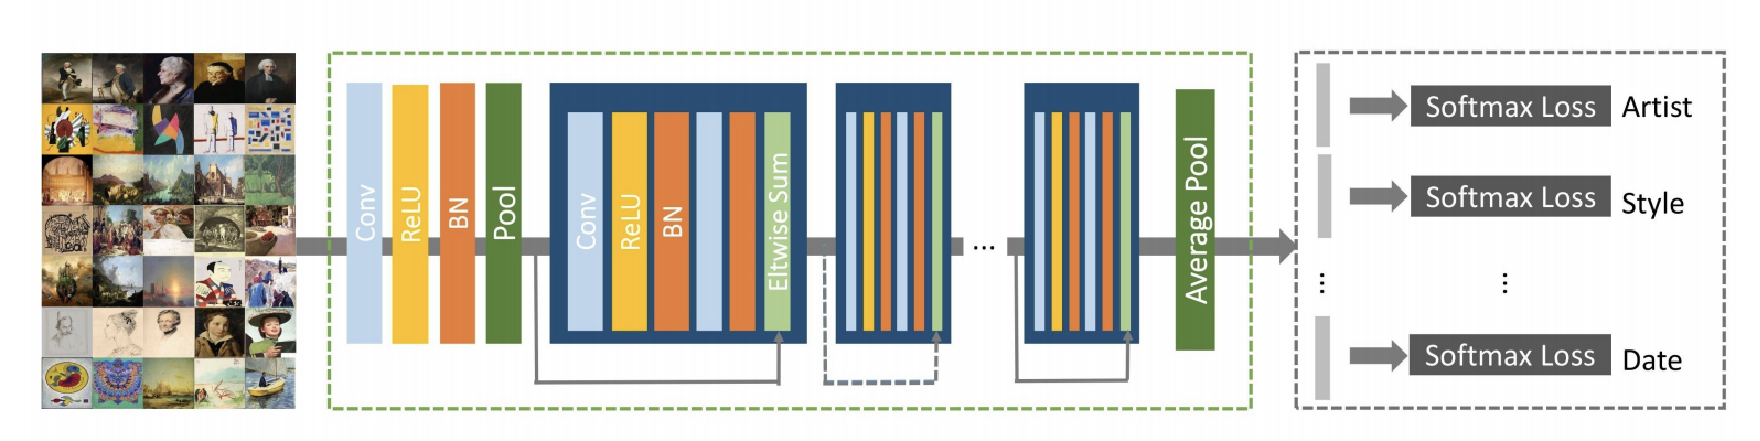
\includegraphics[width=\textwidth]{MTMRmultitask.pdf}
\caption{MTMR's Multitask Learning Structure \cite{parttowhole}}
\label{fig:mtmrmulti}
\end{figure}

Besides the MTMR framework, in 2019, Shen et al. \cite{shen2019discovering} tried to find almost repetitive patterns from a large number of artworks. 

Due to the differences in artistic media (oil paintings, pastel paintings, sketches, etc.) and the inherent deviations in the reproduction process, this goal is more difficult to mine than standard examples. The critical technology is to use self-supervised learning to fine-tune standard depth features on specific art collections to adapt them to this task. Correctly, use spatial consistency between adjacent feature matches as a supervised fine-tuning signal. The adjusted features enable more accurate matching (not affected by differences in style) and can be used with standard pattern discovery methods based on geometric verification to identify repeating patterns in the dataset.

\begin{figure}[h!]
\centering
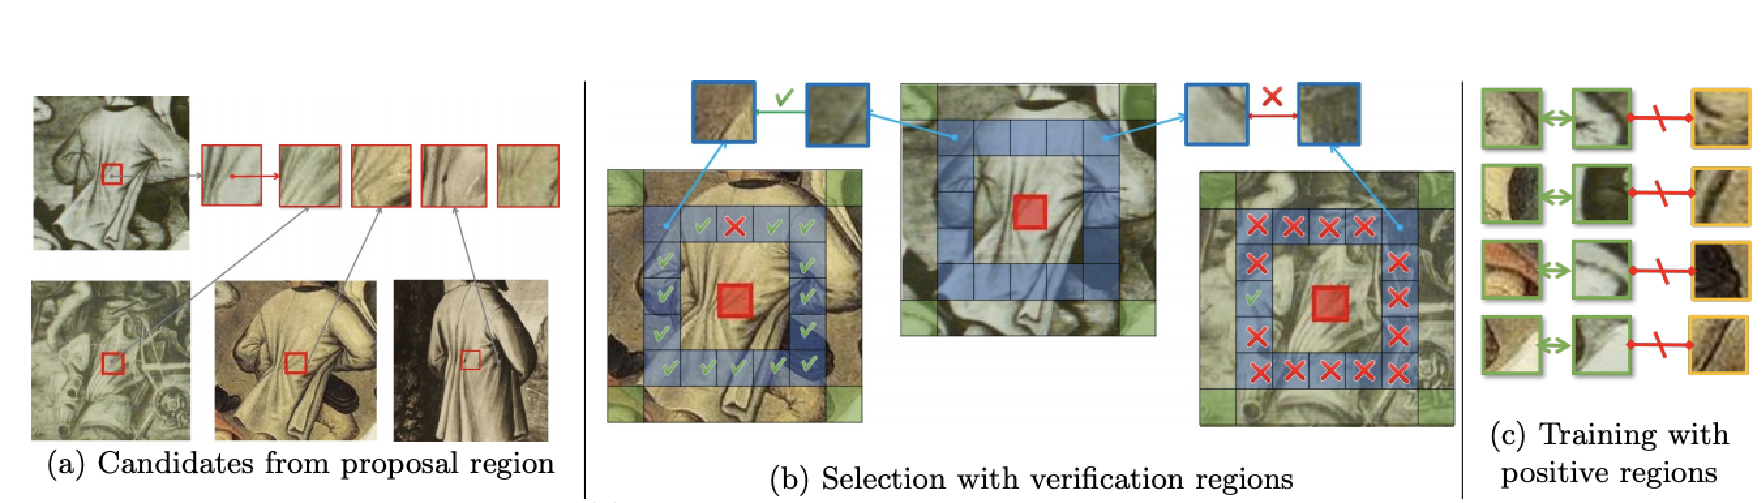
\includegraphics[width=\textwidth]{featurelearningartwork.pdf}
\caption{Feature Learning Strategy \cite{shen2019discovering}}
\label{fig:featurelearning}
\end{figure}

Figure \ref{fig:featurelearning} demonstrates the feature learning process proposed. First candidate correspondences need to be obtained, which come from matching the proposal regions in red boxes with the original complete dataset. Next, these correspondences are checked by comparing features from validation regions (in blue). Finally, only positive results from the previous step will be extracted and kept. 

The method is evaluated on multiple different datasets and showed significant qualitative findings. In terms of quantitative evaluation, the researchers marked 273 approximately repeating details in the dataset of 1,587 works of art by Lao Jan Bruegel and his studio. In addition to works of art, the researchers also showed improvements in the positioning of the algorithm on the \verb|Oxford5K| photo dataset \cite{Philbin07} and historical photo positioning on the LTLL (Large Time Lags Location) dataset \cite{Fernando2015CVIU}.

We believe that a multitasking framework focusing on different levels of features like MTMR \cite{parttowhole} along with a fine-grained feature matching strategies mentioned in Shen et al.'s research \cite{shen2019discovering} will significantly help improve the fine-grained cross modal retrieval model.

\section{Conclusion}
In this section we first presented a fine-grained cross modal retrieval model based on SCAN. It enables image-text retrieval on a fragment level which potentially helped the artwork annotation task. Next, we conducted several experiments under different settings to test the performance of our model on Egyptian and Chinese datasets by comparing their recall rates. To better illustrate and discuss the results, we displayed several successful and unsuccessful retrieval examples from our experiments, which shows our model has the ability to pick common shared features out accurately but sometimes gets stuck on rare and distinctive features. Lack of enough artwork training examples is also suspected as a cause of adequate recalls. We finally pointed future directions on image-text alignment task by analysing recent research works and proposed two major aspects that could possibly benefits our model.

%%% Local Variables: 
%%% mode: latex
%%% TeX-master: "thesis"
%%% End: 

%\chapter{Evaluation}
\label{cha:Evaluation}

\
\chapter{Conclusion}
\label{cha:conclusion}
The final chapter contains the overall conclusion. It also contains
suggestions for future work and industrial applications.

\lipsum[1-7]

%%% Local Variables: 
%%% mode: latex
%%% TeX-master: "thesis"
%%% End: 


% If you have appendices:
%\appendixpage*          % if wanted
\appendix
\chapter{Implementation Details}
\label{app:A}
This appendix provides some \verb|Python| source code for the implementation mentioned in Section \ref{cha:Method}.

\section{Project Structure}
In this section, we go through the structure of my implementation using structured tables. This gives the audience and future researchers a brief idea on how the process looks like.


\begin{table}[h!]
\centering
\begin{tabular}{|l|l|}
\hline
\multicolumn{1}{|c|}{Source Code File} & \multicolumn{1}{c|}{Description}  \\ \hline
\verb|egyptian_convert.py|             & \begin{tabular}[c]{@{}l@{}}Contains \verb|xml| parser and \verb|json| parser. \\ This generates caption for each picture, \\ extract features base on the corresponding \\ caption and also generate features for each \\ image by using parsed \verb|xml| file\end{tabular} \\ \hline
\verb|preprocess.ipynb|                 & \begin{tabular}[c]{@{}l@{}}Combines the features extracted from \\ botton-up attention (Egyptian)\end{tabular}                                                                                                                                          \\ \hline
\verb|chinese_artworks_convert.ipynb| & \begin{tabular}[c]{@{}l@{}}Combines the features extracted from \\ botton-up attention (Chinese)\end{tabular}                                                                                                                                           \\ \hline
\end{tabular}
\label{table:preprocesspython}
\caption{Python Source Code Files for Preprocessing}
\end{table}


%%%%%%%%%%%%%%

\begin{table}[h!]
\centering
\begin{tabular}{|l|l|}
\hline
\multicolumn{1}{|c|}{Source Code File} & \multicolumn{1}{c|}{Description}                                                                                                                             \\ \hline
\verb|data.py|                                & \begin{tabular}[c]{@{}l@{}}Class \verb|PrecompDataset| is where we changed\\ the path of extracted phrases and also where\\ to change process methods.\end{tabular} \\ \hline
\verb|model.py|                               & Provides SCAN model based on VSE++.                                                                                                                           \\ \hline
\verb|train.py|                               & \begin{tabular}[c]{@{}l@{}}Provides training process using settings in\\ \verb|model.py|.\end{tabular}                                                               \\ \hline
\end{tabular}
\label{table:trainpython}
\caption{Python Source Code Files for Training}
\end{table}



%%%%%%%%%%%%%%%

\begin{table}[h!]
\centering
\begin{tabular}{|l|l|}
\hline
\multicolumn{1}{|c|}{Source Code File} & \multicolumn{1}{c|}{Description}                                                                                          \\ \hline
\verb|evaluation.py|                          & \begin{tabular}[c]{@{}l@{}}Provides testing process using the fragment\\ level annotations and ground truth.\end{tabular} \\ \hline
\verb|demo.ipynb|                             & Provides a demo for testing process.                                                                                      \\ \hline
\end{tabular}
\label{table:testpython}
\caption{Python Source Code Files for Testing}
\end{table}


\subsection{Obtain Image Features}
We used bottom-up attention \cite{bottomup} to extract features from our Egyptian and Chinese artwork images. This methodolgy used a faster R-CNN and a ResNet101 as core architecture. We obtained a pre-trained model from its \href{https://github.com/peteanderson80/bottom-up-attention}{Github} open repository which was trained on \verb|VisualGenome| dataset consisting a large amount of real-world images. A sample image feature extraction command for Egyptian training images is displayed below:

\begin{lstlisting}
$ python bottom-up-features/extract_features.py 
--image_dir artworks/train --out_dir artworks/features 
--cfg bottom-up-features/cfgs/faster_rcnn_resnet101.yml 
--model bottom-up-features/models/bottomup_pretrained_10_100.pth
\end{lstlisting}

We save these obtained image features under \verb|/features| directory. These image features of Egyptian and Chinese artworks are available in numpy array format, which can be used for training directly in the future.

\subsection{Obtain Textual Features}

According to captions and corresponding image labels, we can extract the corresponding image names from \verb|xml| and \verb|json| files which contains textual attributes. This extraction process can be done using \verb|egyptian_convert.py|, \verb|python| script then generates captions for each image, make sure that each has a corresponding \verb|.txt| file created. These produced \verb|.txt| files are saved in \verb|/phrase| directory. 

To achieve the retrieval on a fragment level, we then extract noun phrases from these \verb|.txt| files. We use \verb|/preprocess.ipynb| to obtain \verb|vocab.json|. The API adopted here was proposed by Handler et al. \cite{nounphrase} and available on \href{https://github.com/slanglab/phrasemachine}{Github} as well.

\subsection{Training and Testing}
For training process, we can simply modify the \verb|PrecompDataset| class in \verb|data.py| to change related processing methods. A sample training command for Chinese training images is displayed below (with i-t average pooling formulation):

\begin{lstlisting}
python train.py --data_name chinese_artworks 
--logger_name $RUN_PATH/chinese_artworks_scan/log 
--model_name $RUN_PATH/chinese_artworks_scan/log 
--max_violation --bi_gru --img_dim 2048
--agg_func=Mean --cross_attn=i2t --lambda_softmax=4
\end{lstlisting}

For testing process, we load our saved model then run \verb|evaluation.py| script. A sample evaluation command is shown below:

\begin{lstlisting}[language=python]
from vocab import Vocabulary
import evaluation
evaluation.evalrank("$RUN_PATH/chinese_artworks_scan/model_best.pth.tar", data_path="$DATA_PATH", split="test")
\end{lstlisting}


%%%%%%%%%%%%%%

\section{Python Snippets}
In this section, we briefly display the preprocessing part of our implementation which is also crucial to the entire project as an efficient and accuracy extraction from \verb|xml| files can make the training and testing process easier and more smooth.

Here we focus on two specific files, one is \verb|egyptian_convert.py| which is able to parse \verb|xml| and \verb|json| files. Another one is \verb|preprocess.ipynb| which combines features and vocabularies for each distinct artwork.


\subsection{Texual Attribute Parser}

Here the code snippet of \verb|egyptian_convert.py| is displayed below. Similarly, \verb|chinese_artwork_convert.py| works for Chinese artwork dataset.

\begin{lstlisting}[language=Python]
import xml.etree.ElementTree as ET
import os
import numpy as np
from tqdm import tqdm
import json

# this module used to generate caption for each picture and extract features base on the corresponding caption

# parse the xml and get the text for relevant element

def get_text(path):
    tree = ET.parse(path)
    root = tree.getroot()
    file_name = root[1].text
    res = []
    for object in tree.findall("object"):
        res.append(object[0].text)
    return file_name,res

# generate features for each image by using parsed xml file

def xml_parser(path,features_path,save_path):
    list_dir = os.listdir(path)
    features = []
    not_list = []
    for image in tqdm(list_dir):
        file_path = os.path.join(features_path, image.split('.')[0] + '.npy')
        feature = np.load(file_path, allow_pickle=True).tolist()["features"]
        print(feature)
        feature = np.array(feature)
        features.append(feature[:10, :])
    features = np.stack(features)
    np.save(save_path, features)
    
def json_parser(path):

    # load the json files extract the sentence and corresponding picture name.
    
    with open(path,"r") as file:
        data = json.load(file)
        for image in data["images"]:
            try:
                file_name = image["filename"]+".txt"
                sentence = image["sentences"]
                sentence = sentence[0]["raw"]
            except:
                continue
            # save the sentence in relevant files
            with open(os.path.join("../data/phrase_train", file_name),"w") as f:
                f.write(sentence)
                
\end{lstlisting}

\subsection{Feature Combination}
Here the code snippet of \verb|preprocess.ipynb| is displayed below.

\begin{lstlisting}[language=Python]
import torchvision
import torch
import json
import cv2
import os.path as osp
from PIL import Image
from tqdm import tqdm_notebook
import numpy as np
import nltk
from collections import Counter

# combine the features extracted from botton-up attention

content = json.load(open(osp.join(dataset_name, 'caption_data.json')))

images = {
    'train': [],
    'test': [],
    'val': []
}

for image in content['images']:
    filepath = image['filepath']
    if len(image['sentences']) == 0:
        continue
    images[filepath].append(image)
    
for phase in images.keys():
    features = []
    for image in tqdm_notebook(images[phase]):
        file_path = osp.join(dataset_name, 'features', image['filename'].split('.')[0] + '.npy')
        print(file_path)
        feature = np.load(file_path)
        features.append(feature[:10, :])
    features = np.stack(features)
    np.save(osp.join(dataset_name, phase), features)

from vocab import Vocabulary, serialize_vocab
from collections import Counter
import phrasemachine

threshold = 4
counter = {}
for phase in images.keys():
    captions = [x['sentences'][0]['raw'] for x in images[phase]]
    for caption in captions:
        temp = list(phrasemachine.get_phrases(caption)["counts"].keys())
        for key in temp:
            if key not in counter.keys():
                counter[key] = 1
            else:
                counter[key] += 1
# Discard if the occurrence of the word is less than min_word_cnt.
words = [word for word, cnt in counter.items() if cnt >= threshold]

# create a vocab wrapper and add some special tokens
vocab = Vocabulary()
vocab.add_word('<pad>')
vocab.add_word('<start>')
vocab.add_word('<end>')
vocab.add_word('<unk>')

# Add words to the vocabulary.
for i, word in enumerate(words):
    vocab.add_word(word)
serialize_vocab(vocab, osp.join(dataset_name, 'vocab.json'))

with open(osp.join(dataset_name, 'data.json'), 'w') as f:
    json.dump(images, f)
\end{lstlisting}


%%% Local Variables: 
%%% mode: latex
%%% TeX-master: "thesis"
%%% End: 

% ... and so on until
%\chapter{Experiment Details}
\label{app:n}
details

\section{Training Settings}



%%% Local Variables: 
%%% mode: latex
%%% TeX-master: "thesis"
%%% End: 


\backmatter
% The bibliography comes after the appendices.
% You can replace the standard "abbrv" bibliography style by another one.
\bibliographystyle{abbrv}
\bibliography{references}

\end{document}

%%% Local Variables: 
%%% mode: latex
%%% TeX-master: t
%%% End: 
